\documentclass[UTF8,a4paper,12pt]{ctexart}
\usepackage[margin=2.5cm]{geometry}
\usepackage{graphicx}
\usepackage{booktabs}
\usepackage{longtable}
\usepackage{tabularx}
\usepackage{array}
\usepackage{calc}
\usepackage{textcomp}
\usepackage{amsmath}
\usepackage{amssymb}
\usepackage{enumitem}
\usepackage{caption}
\usepackage{fancyhdr}
\usepackage{listings}
\usepackage{float}
\usepackage[hidelinks]{hyperref}
\usepackage{color}
\usepackage{tikz}
\usepackage{tikz-cd}

\usepackage{dirtree}
\usepackage{xcolor}

\usetikzlibrary{shapes.geometric, arrows.meta, positioning, calc}

\setcounter{tocdepth}{3}
\setlength{\parindent}{2em}
\setlength{\parskip}{0.35em}
\setlist{itemsep=0.2em, topsep=0.3em, parsep=0pt, partopsep=0pt}
\renewcommand{\arraystretch}{1.2}
\graphicspath{{src/assets/}{assets/}}
\captionsetup{font=small,labelfont=bf,position=bottom}
\captionsetup[table]{position=top,skip=6pt}
\pagestyle{fancy}
\fancyhf{}
\fancyfoot[C]{\thepage}
\renewcommand{\headrulewidth}{0pt}
\renewcommand{\footrulewidth}{0pt}
\newcolumntype{L}[1]{>{\raggedright\arraybackslash}p{#1}}
\newcolumntype{C}[1]{>{\centering\arraybackslash}p{#1}}
\newenvironment{threelongtable}[1]{%
  \setlength\LTleft{\fill}%
  \setlength\LTright{\fill}%
  \renewcommand{\arraystretch}{1.2}%
  \scriptsize
  \begin{longtable}{#1}%
}{%
  \end{longtable}%
}
\lstdefinelanguage{SystemVerilog}{
  morekeywords={module,endmodule,input,output,wire,reg,assign,always,begin,end,if,else,casez,default},
  sensitive=true,
  morecomment=[l]{//},
  morecomment=[s]{/*}{*/},
  morestring=[b]"
}
\lstdefinestyle{svcode}{
  language=SystemVerilog,
  basicstyle=\ttfamily\scriptsize,
  keywordstyle=\bfseries\color{blue},
  commentstyle=\color{gray},
  numbers=none,
  breaklines=true,
  columns=fullflexible,
  keepspaces=true,
  frame=tb,
  showstringspaces=false,
  captionpos=b,
  aboveskip=0.8em,
  belowskip=0.8em
}
\lstset{basicstyle=\ttfamily\small,breaklines=true,columns=fullflexible,frame=single}
\newcommand{\coverfield}[2]{%
  {\zihao{4}%\heiti
   \noindent\makebox[6em][l]{\heiti#1：}%
   \underline{\makebox[\dimexpr\textwidth-6em\relax][l]{\strut\heiti #2}}\par}%
}

\title{基于RISC-V指令集的CPU设计\\竞业达分赛区决赛技术文档}
\author{队伍编号：CICC1004252\\团队名称：和溢位}
\date{}

\begin{document}
\begin{titlepage}
  \centering
  
\includegraphics[width=0.35\textwidth]{common/image1.png}\par\vspace{1.2cm}
  {\zihao{2}\bfseries 第十届\\全国大学生集成电路创新创业大赛\par}
  \vspace*{\fill}
  \begin{minipage}{\textwidth}
    \raggedright
    \setlength{\parindent}{0pt}
    \coverfield{报告类型}{分赛区决赛技术文档}
    \vspace{0.45cm}
    \coverfield{参赛杯赛}{``竞业达"企业命题}
    \vspace{0.45cm}
    \coverfield{作品名称}{基于RISC-V指令集的CPU设计}
    \vspace{0.45cm}
    \coverfield{队伍编号}{CICC1004252}
    \vspace{0.45cm}
    \coverfield{团队名称}{和溢位}
    \vspace{2cm}
  \end{minipage}
\end{titlepage}

\tableofcontents
\clearpage

\section*{作品核心内容快速预览}
\addcontentsline{toc}{section}{作品核心内容快速预览}

本项目在初赛 RV32I 五级流水 CPU 的基础上完成分赛区决赛版本迭代。处理器采用
IFU--IDU--EXU--LSU--WBU 五级顺序单发射架构，支持赛题所需的 37 条 RV32I 指令，
并扩展 RV32M、Zicsr 六条 CSR 读改写指令以及 \texttt{ECALL}/\texttt{MRET} 机器态控制流。
设计加入多周期乘除法、2 KiB 直映射 D-cache、基于 FPGA 分布式 RAM 的双副本寄存器堆，
并通过连续取指、16 项 BTB、译码级预计算和关键路径拆分提升频率与有效吞吐率。

工程在 Xilinx Kintex-7 XC7K325T-2FFG900 平台和 Vivado 2024.2 下完成综合、实现与上板验证，
核心频率达到 \textcolor{red}{\textbf{280 MHz}}，布局布线后 WNS 为
\textcolor{red}{\textbf{+0.050 ns}}，无建立时间违例。官方 \texttt{src0}、\texttt{src1}、
\texttt{src2} 的上板运行时间分别为 \textbf{7.101 s、7.047 s、9.233 s}；
\texttt{withoutMext} 与 \texttt{withMext} 分别用时 \textbf{3.890 s、2.020 s}，
硬件 M 扩展获得约 \textbf{1.93 倍}加速。

验证体系由 Vivado Simulation 与 Verilator/C++ 双平台组成，通过 DPI-C 支持停机检测和外设模拟，
以 NEMU 作为差分测试参考模型，并接入 GitHub Actions 持续集成。验证覆盖 RV32I、RV32M、Zicsr、
官方性能程序、CoreMark、Dhrystone 和 RT-Thread 基础负载；仿真预测用时与上板结果一致，
形成从指令级测试、性能量化到数字孪生上板的完整验证闭环。

\begin{figure}[H]
  \centering
  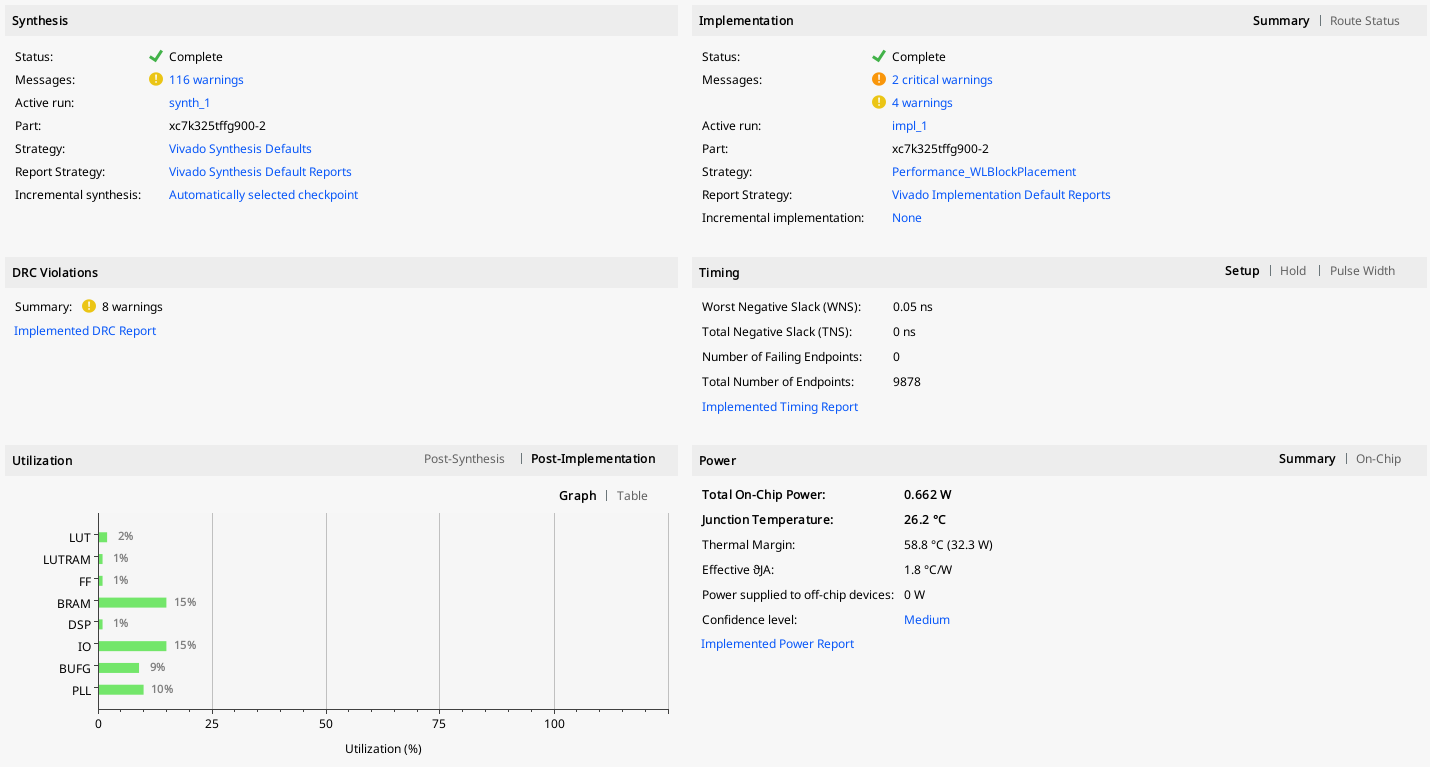
\includegraphics[width=0.96\linewidth]{common/快速预览-1.png}\\[0.5em]
  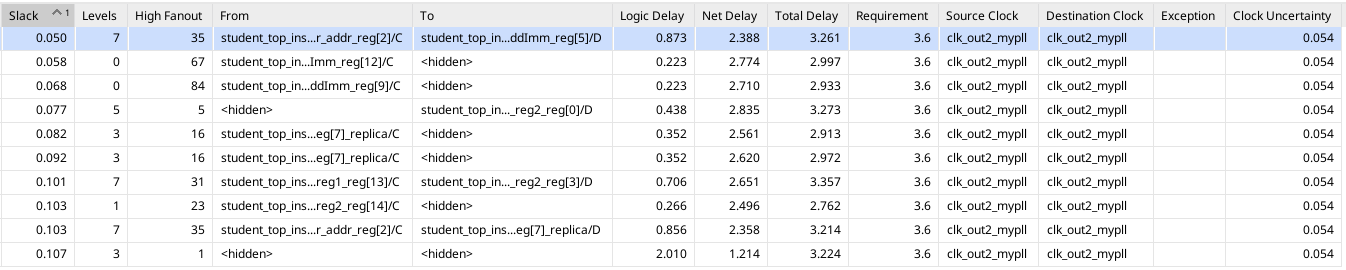
\includegraphics[width=0.96\linewidth]{common/快速预览-slack.png}
  \caption{分赛区决赛版本核心指标与时序结果}
\end{figure}

\clearpage

\section{项目概述}

\subsection{项目背景}

``竞业达''企业命题要求参赛队伍完成一款能够在指定 FPGA 平台上运行的
RISC-V CPU，并最终在``竞业达''官方定制 FPGA
平台上板验证。围绕这一目标，本项目完成了
CPU 内核与简易 SoC 设计，将赛方测试程序配置到板端 IROM/DRAM
并成功完成最终运行。

\subsection{设计目标}

本项目的设计目标包括：实现支持 RV32I 指令集的 RISC-V 处理器；完成
IROM、DRAM 和 MMIO 的统一地址映射；在 FPGA 顶层接入
LED、数码管和计数器等板级资源；保证最终版工程能够在 Vivado 2024.2
下完成实现，并通过数字孪生平台完成 \texttt{src0}、\texttt{src1}、\texttt{src2}、
\texttt{withoutMext} 与 \texttt{withMext} 的运行验证。

\subsection{设计平台说明}

本设计使用 Vivado 2024.2 版本进行综合、实现。

硬件平台为``竞业达''官方基于 Kintex-7 定制的 FPGA 开发板，CPU
核心工作频率为 280 MHz，布局布线后的 WNS 为 +0.050 ns，无建立时间违例。

采用 SystemVerilog 语言进行设计，并使用了 Chisel
完成部分模块的辅助生成，以提高设计抽象层次与开发效率。

% \newpage

\section{RISC-V CPU 架构设计}

\subsection{指令集支持情况}

当前支持赛题所需的 37 条 RV32I 整数、访存与控制流指令，并扩展支持 RV32M、Zicsr 六条
CSR 读改写指令，以及 \texttt{ECALL}/\texttt{MRET} 机器态控制流。

\begin{threelongtable}{@{}
  >{\raggedright\arraybackslash}p{(\linewidth - 4\tabcolsep) * \real{0.2}}
  >{\raggedright\arraybackslash}p{(\linewidth - 4\tabcolsep) * \real{0.4}}
  >{\raggedright\arraybackslash}p{(\linewidth - 4\tabcolsep) * \real{0.4}}@{}}
\caption{RISC-V 指令支持情况}\\
\toprule\noalign{}
\begin{minipage}[b]{\linewidth}\centering
\textbf{类别}
\end{minipage} & \begin{minipage}[b]{\linewidth}\centering
\textbf{典型指令/功能}
\end{minipage} & \begin{minipage}[b]{\linewidth}\centering
\textbf{说明}
\end{minipage} \\
\midrule\noalign{}
\endhead
\bottomrule\noalign{}
\endlastfoot
寄存器运算 & ADD, SUB, SLL, SLT, SLTU, XOR, SRL, SRA, OR, AND &
由 EXU 中 ALU 完成 \\
立即数运算 & ADDI, SLTI, SLTIU, XORI, ORI, ANDI, SLLI, SRLI/SRAI & 由
IDU 生成立即数，EXU 送入 ALU 完成 \\
访存指令 & LB, LH, LW, LBU, LHU, SB, SH, SW & EXU 生成读写请求，LSU/WBU
完成读结果处理 \\
控制流 & BEQ, BNE, BLT, BGE, BLTU, BGEU, JAL, JALR & EXU
中判定分支预测正误并拉起重定向PC信号 \\
高位立即数 & LUI, AUIPC & 直接形成写回数据 \\
M 扩展 & MUL, MULH, MULHSU, MULHU, DIV, DIVU, REM, REMU &
由 EXU 中多周期乘法、除法 IP 完成，使用 ready/valid 握手 \\
Zicsr & CSRRW, CSRRS, CSRRC, CSRRWI, CSRRSI, CSRRCI &
IDU 读 CSR、EXU 形成新值、WBU 顺序提交 \\
系统相关 & ECALL, MRET & CSR 堆与机器态异常返回路径 \\
\end{threelongtable}

\subsection{CPU 整体架构图}

CPU
内核由取指（IFU）、译码（IDU）、执行与访存发起（EXU）、访存响应（LSU）和
写回（WBU）五个主要阶段组成；同时设置独立的寄存器堆、CSR
堆、分支目标缓存和外设桥。对竞业达平台的适配主要体现在 FPGA
顶层的存储器封装和外设桥 MMIO 地址映射。

% \begin{figure}[htbp]
% \centering
% 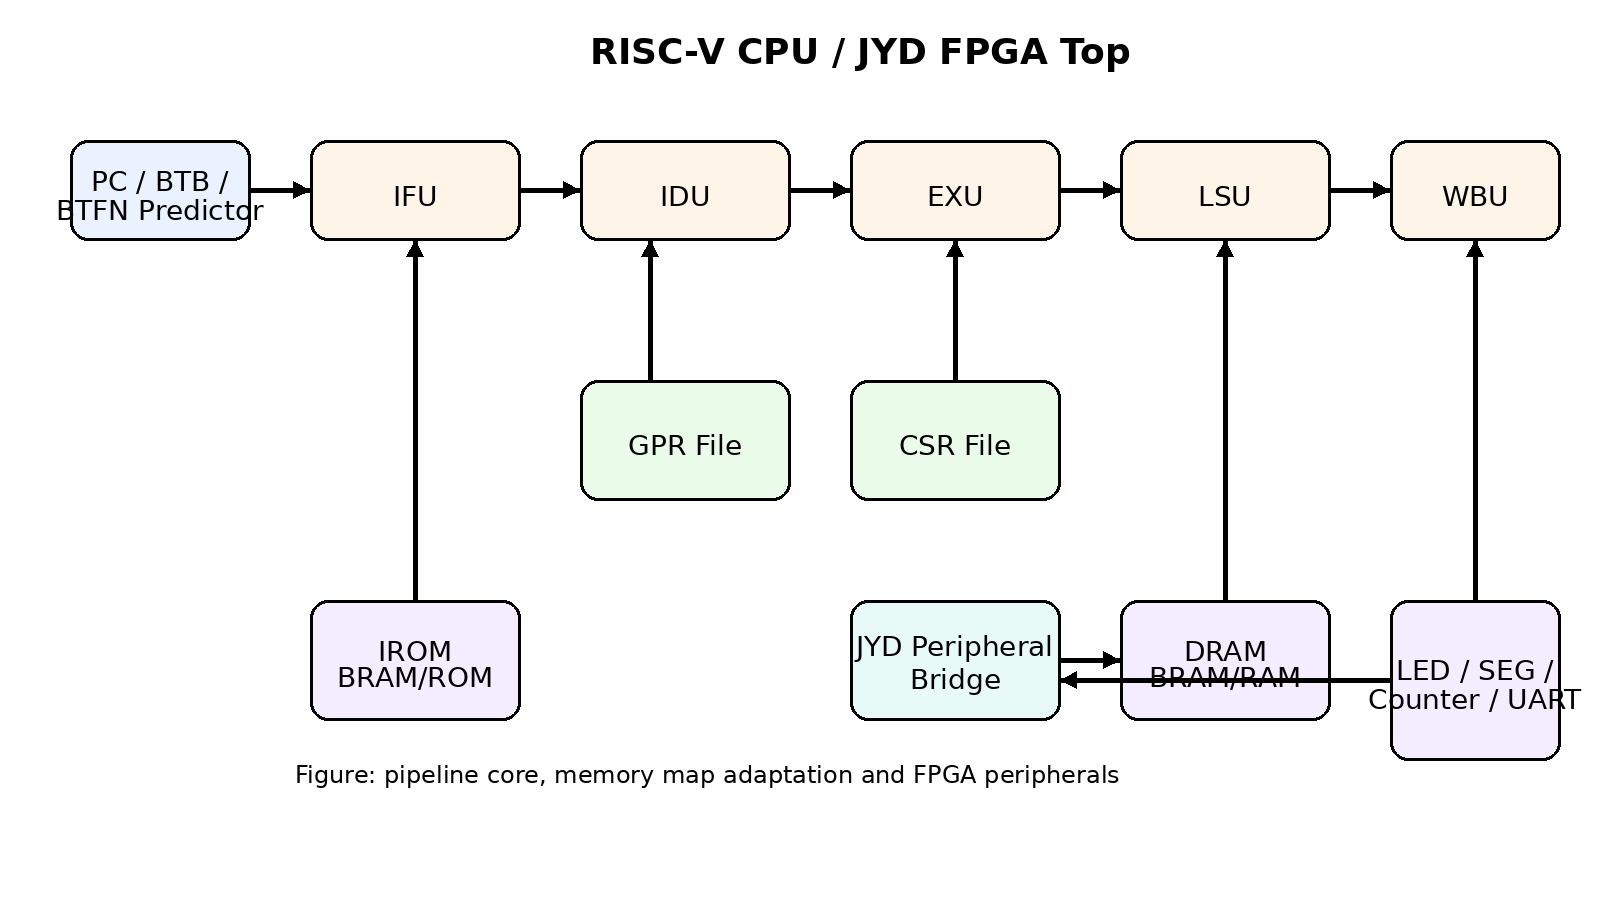
\includegraphics[width=0.96\linewidth]{design/image4.png}
% \caption{CPU核心与竞业达 FPGA 顶层适配关系示意图}
% \end{figure}

\begin{figure}[H]
  \centering
	
\includegraphics[width=\textwidth,trim={15pt 130pt 15pt 45pt},clip]{design/cpu-arch.pdf}
	\caption{架构图}
\end{figure}

图中给出了分赛区决赛版本的完整架构。设计仍保持原有五级主流水，并在 EXU 中接入多周期乘除法
单元，在数据侧加入 2 KiB D-cache，同时使用 FPGA 分布式 RAM IP 实现通用寄存器堆；这些变化
不改变 IFU 的状态机、连续取指方式和主流水级划分。

\subsection{数据通路各模块的设计}

CPU
数据通路遵循``指令在流水线中逐级传递、控制信息与数据信息同时随指令流动''的设计思路。各模块的职责如下。

\subsubsection{IFU 取指模块}

IFU 作为前端取指单元，负责将 PC 转化为实际取指请求并输出带有
PC、预测信息和指令编号的 FetchedInst，并尽可能保持每周期连续取指。

\begingroup
\setlength\LTleft{\fill}
\setlength\LTright{\fill}
\small
\renewcommand{\arraystretch}{1.2}
\begin{longtable}{@{}
  >{\raggedright\arraybackslash}p{(\linewidth - 4\tabcolsep) * \real{0.2}}
  >{\raggedright\arraybackslash}p{(\linewidth - 4\tabcolsep) * \real{0.1}}
  >{\raggedright\arraybackslash}p{(\linewidth - 4\tabcolsep) * \real{0.7}}@{}}
\caption{IFU 接口信号说明}\\
\toprule\noalign{}
\begin{minipage}[b]{\linewidth}\raggedright
接口
\end{minipage} & \begin{minipage}[b]{\linewidth}\raggedright
方向
\end{minipage} & \begin{minipage}[b]{\linewidth}\raggedright
作用
\end{minipage} \\
\midrule\noalign{}
\endhead
\bottomrule\noalign{}
\endlastfoot
pc & 输入 & 上游给出的待取指地址 \\
predNext & 输入 & 该条指令对应的预测元信息 \\
mem & 输出 & 对取指存储端口发起 SimpleBus 读请求 \\
out & 输出 & 向 IDU 输出 FetchedInst \\
\end{longtable}
\endgroup

其中 FetchedInst 除指令本身外，还携带：当前 pc、预测信息
pred、单调递增的 指令编号 iid。

当前实现使用 4
个状态的状态机处理请求、等待和反压节拍。状态分别为空闲（Idle）、等待访存接受请求（WaitReq）、等待访存返回数据（WaitResp）、等待后级反压结束可以接受新指令数据（WaitOut）。

% https://q.uiver.app/#q=WzAsNyxbMCwwLCJcXHRleHR7SWRsZX0iXSxbMCwyLCJcXHRleHR7V2FpdFJlcX0iXSxbNiwyLCJcXHRleHR7V2FpdFJlc3B9Il0sWzYsMCwiXFx0ZXh0e1dhaXRPdXR9Il0sWzAsMSwiXFxidWxsZXQiXSxbMywwLCJcXGNpcmMiXSxbMywyLCJcXGNpcmMiXSxbNCwwLCJcXHRleHRybXtSZXNldH0iXSxbMiw1LCJcXHRleHRybXtNRU0gYWNjZXB0ZWR9IiwxLHsic3R5bGUiOnsiaGVhZCI6eyJuYW1lIjoiZXBpIn19fV0sWzUsMCwiXFx0ZXh0cm17Tm8gbmV3IHZhbGlkIFBDfSJdLFs1LDYsIlxcdGV4dHJte0hhcyBuZXcgUEN9IiwxLHsic3R5bGUiOnsiaGVhZCI6eyJuYW1lIjoiZXBpIn19fV0sWzYsMiwiXFx0ZXh0cm17TUVNIGFjY2VwdGVkfSIsMV0sWzYsMSwiXFx0ZXh0cm17TUVNIG5vdCByZWFkeX0iLDIseyJvZmZzZXQiOjF9XSxbMSw2LCJcXHRleHRybXtNRU0gYWNjZXB0ZWR9IiwyLHsib2Zmc2V0IjoxLCJzdHlsZSI6eyJoZWFkIjp7Im5hbWUiOiJlcGkifX19XSxbMyw1LCJcXHRleHRybXtPdXQgcmVhZHl9IiwwLHsic3R5bGUiOnsiaGVhZCI6eyJuYW1lIjoiZXBpIn19fV0sWzAsNSwiXFx0ZXh0cm17SGFzIG5ldyBQQ30iLDAseyJvZmZzZXQiOi0yLCJzdHlsZSI6eyJoZWFkIjp7Im5hbWUiOiJlcGkifX19XSxbNSwzLCJcXHRleHRybXtPdXQgbm90IHJlYWR5fSIsMCx7Im9mZnNldCI6LTJ9XV0=
\begin{figure}[htbp]
\centering
\begin{tikzcd}
	{\text{Idle}} &&& \circ &&& {\text{WaitOut}} \\
	\bullet \\
	{\text{WaitReq}} &&& \circ &&& {\text{WaitResp}}
	\arrow["{\textrm{Has new PC}}", shift left=2, two heads, from=1-1, to=1-4]
	\arrow["{\textrm{No new valid PC}}", from=1-4, to=1-1]
	\arrow["{\textrm{Out not ready}}", shift left=2, from=1-4, to=1-7]
	\arrow["{\textrm{Has new PC}}"{description}, two heads, from=1-4, to=3-4]
	\arrow["{\textrm{Out ready}}", two heads, from=1-7, to=1-4]
	\arrow["{\textrm{Reset}}", from=2-1, to=1-1]
	\arrow["{\textrm{MEM accepted}}"', shift right, two heads, from=3-1, to=3-4]
	\arrow["{\textrm{MEM not ready}}"', shift right, from=3-4, to=3-1]
	\arrow["{\textrm{MEM accepted}}"{description}, from=3-4, to=3-7]
	\arrow["{\textrm{MEM accepted}}"{description}, two heads, from=3-7, to=1-4]
\end{tikzcd}
\caption{IFU 状态机的简化状态转移图}
\end{figure}

其中 $\circ$ 表示MUX选择而非状态，具体的状态转移布尔表达式见下图

% https://q.uiver.app/#q=WzAsNSxbMSwwLCJcXHRleHR7SWRsZX0iXSxbMCw0LCJcXHRleHR7V2FpdFJlcX0iXSxbMCwwLCJcXGJ1bGxldCJdLFs3LDAsIlxcdGV4dHtXYWl0UmVzcH0iXSxbOCw0LCJcXHRleHR7V2FpdE91dH0iXSxbMCwxLCJcXHJtIFZhbGlkX3tQQ30gXFxsYW5kIFxcbG5vdCBSZWFkeV97bWVtLnJlcX0iLDJdLFswLDAsIlxcbG5vdCBcXHJtIFZhbGlkX3tQQ30iXSxbMiwwXSxbMywwLCJcXHJtIFZhbGlkX3ttZW0ucmVzcH0gXFxsYW5kIFJlYWR5X3tvdXR9XFxsYW5kXFxsbm90IFZhbGlkX3tQQ30iLDAseyJvZmZzZXQiOi0xfV0sWzAsMywiXFxybSBWYWxpZF97UEN9IFxcbGFuZCBSZWFkeV97bWVtLnJlcX0iLDAseyJvZmZzZXQiOi0xfV0sWzQsMCwiXFxybSBSZWFkeV97b3V0fSBcXGxhbmQgXFxsbm90IFZhbGlkX3tQQ30iLDEseyJsYWJlbF9wb3NpdGlvbiI6NDB9XSxbMSwzLCJcXHJtIFJlYWR5X3ttZW0ucmVxfSIsMCx7ImxhYmVsX3Bvc2l0aW9uIjo0MCwib2Zmc2V0IjoxfV0sWzEsMSwiXFxybSBcXGxub3QgUmVhZHlfe21lbS5yZXF9IiwwLHsiYW5nbGUiOi0xODB9XSxbMywxLCJcXHJte1ZhbGlkX3ttZW0ucmVzcH0gXFxsYW5kIFJlYWR5X3tvdXR9fVxcbGFuZCBWYWxpZF97UEN9IFxcbGFuZCBcXGxub3QgUmVhZHlfe21lbS5yZXF9IiwwLHsib2Zmc2V0IjotM31dLFs0LDEsIlxccm0gUmVhZHlfe291dH1cXGxhbmQgVmFsaWRfe1BDfVxcbGFuZCBcXGxub3QgUmVhZHlfe21lbS5yZXF9IiwwLHsib2Zmc2V0IjotMX1dLFszLDQsIlxccm0gVmFsaWRfe21lbS5yZXNwfSBcXGxhbmQgXFxsbm90IFJlYWR5X3tvdXR9Il0sWzMsMywiXFxybVxcbG5vdCBWYWxpZF97bWVtLnJlc3B9IFxcbG9yICggUmVhZHlfe291dH1cXGxhbmQgVmFsaWRfe1BDfSBcXGxhbmQgUmVhZHlfe21lbS5yZXF9KSJdLFs0LDMsIlxccm0gUmVhZHlfe291dH1cXGxhbmQgVmFsaWRfe1BDfVxcbGFuZCBSZWFkeV97bWVtLnJlcX0iLDEseyJsYWJlbF9wb3NpdGlvbiI6ODAsIm9mZnNldCI6LTJ9XSxbNCw0LCJcXHJtIFxcbG5vdCBSZWFkeV97b3V0fSIsMCx7ImFuZ2xlIjoxODB9XV0=
\begin{figure}[htbp]
\centering
\begin{tikzcd}
	\bullet & {\text{Idle}} &&&&&& {\text{WaitResp}} \\
	\\
	\\
	\\
	{\text{WaitReq}} &&&&&&&& {\text{WaitOut}}
	\arrow[from=1-1, to=1-2]
	\arrow["{\lnot \rm Valid_{PC}}", from=1-2, to=1-2, loop, in=55, out=125, distance=10mm]
	\arrow["{\rm Valid_{PC} \land Ready_{mem.req}}", shift left, from=1-2, to=1-8]
	\arrow["{\rm Valid_{PC} \land \lnot Ready_{mem.req}}"', from=1-2, to=5-1]
	\arrow["{\rm Valid_{mem.resp} \land Ready_{out}\land\lnot Valid_{PC}}", shift left, from=1-8, to=1-2]
	\arrow["{\rm\lnot Valid_{mem.resp} \lor ( Ready_{out}\land Valid_{PC} \land Ready_{mem.req})}", from=1-8, to=1-8, loop, in=55, out=125, distance=10mm]
	\arrow["{\rm{Valid_{mem.resp} \land Ready_{out}}\land Valid_{PC} \land \lnot Ready_{mem.req}}"{pos=0.75}, shift left=3, from=1-8, to=5-1]
	\arrow["{\rm Valid_{mem.resp} \land \lnot Ready_{out}}", from=1-8, to=5-9]
	\arrow["{\rm Ready_{mem.req}}"{pos=0.4}, shift right, from=5-1, to=1-8]
	\arrow["{\rm \lnot Ready_{mem.req}}", from=5-1, to=5-1, loop, in=235, out=305, distance=10mm]
	\arrow["{\rm Ready_{out} \land \lnot Valid_{PC}}"{description, pos=0.4}, from=5-9, to=1-2]
	\arrow["{\rm Ready_{out}\land Valid_{PC}\land Ready_{mem.req}}"{description, pos=0.8}, shift left=2, from=5-9, to=1-8]
	\arrow["{\rm Ready_{out}\land Valid_{PC}\land \lnot Ready_{mem.req}}", shift left, from=5-9, to=5-1]
	\arrow["{\rm \lnot Ready_{out}}", from=5-9, to=5-9, loop, in=235, out=305, distance=10mm]
\end{tikzcd}
\caption{IFU 状态机的完整转移条件}
\end{figure}

若当前周期
IFU 已经准备接受新 PC，但存储端 req\_ready 还未就绪，则
PC 会先进入 pending 路径保存；对应的预测信息和 iid 一并保存；等待后续存储端可接收时再真正发起请求。保证前端不会因为总线短暂背压而丢失刚接到的新负载。

waitResp 状态下若访存响应在当周期返回、且 IDU 也在当周期接收成功，则 IFU
可以立刻接入下一条 PC 并尝试发起下一次请求。
也就是说，下面三件事可以在一个周期中发生： 
消费上一条取指结果；
接收下一条 PC；
发起下一次请求。

从而隐藏了使用BRAM作为 IROM 的一周期延迟，表现出来仍能每周期取指令。

\begin{figure}[htbp]
\centering
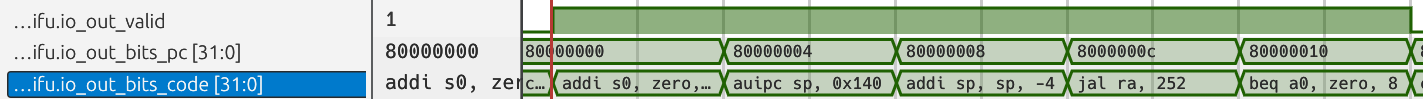
\includegraphics[width=0.96\linewidth]{design/imaged.png}\\[0.5em]
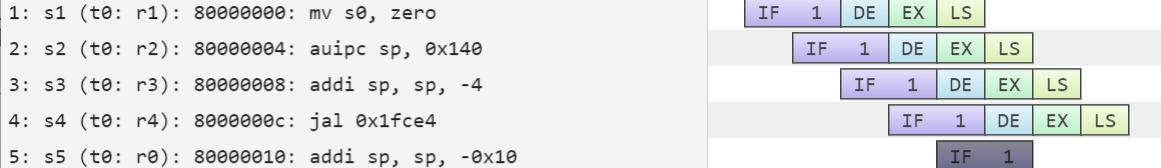
\includegraphics[width=0.88\linewidth]{design/imagee.png}
\caption{IFU 连续取指与 BRAM 延迟隐藏仿真波形}
\end{figure}

预测结果不在后端重新查询，而是和指令一起进入流水线。这样 EXU
能直接对照该条指令的预测记录做校验。

\subsubsection{IDU 译码与寄存器读取模块}

IDU 包含译码、访问寄存器堆、旁路、预计算功能。

\begin{threelongtable}{@{}
  >{\raggedright\arraybackslash}p{(\linewidth - 4\tabcolsep) * \real{0.2}}
  >{\raggedright\arraybackslash}p{(\linewidth - 4\tabcolsep) * \real{0.1}}
  >{\raggedright\arraybackslash}p{(\linewidth - 4\tabcolsep) * \real{0.7}}@{}}
\caption{IDU 接口信号说明}\\
\toprule\noalign{}
\begin{minipage}[b]{\linewidth}\raggedright
接口
\end{minipage} & \begin{minipage}[b]{\linewidth}\raggedright
方向
\end{minipage} & \begin{minipage}[b]{\linewidth}\raggedright
作用
\end{minipage} \\
\midrule\noalign{}
\endhead
\bottomrule\noalign{}
\endlastfoot
in & 输入 & 来自 IFU 的 FetchedInst \\
rvec & 输出 & 读取两个 GPR 源寄存器 \\
csrRead & 输出 & 读取当前指令需要访问的 CSR \\
csrJmpTarget & 输入 & 提供 mepc/mtvec \\
wrBackInfo & 输入 & 来自 EXU/LSU/WBU 的旁路信息 \\
pipelineFlush & 输入 & 上游通知当前路径是否被清空 \\
out & 输出 & 送往 EXU 的 DecodedInst \\
\end{threelongtable}

译码功能会根据 opcode 将指令粗分为 imm、reg、store、upper、jump、branch
等格式，以及 arithmetic、load、store、jal、jalr、lui、auipc、system
等类型，并生成 I/S/B/U/J 五类立即数，根据指令类型格式选取IMM。

访问寄存器会同时发起双读端口 GPR 访问和单读端口 CSR 访问。

旁路网络通过 \texttt{ByPassMux}
同时观察来自以下三个位置的写回信息：EXU、LSU、WBU

\begin{figure}[htbp]
\centering
\resizebox{0.88\linewidth}{!}{%
\begin{tikzpicture}[
  node distance=0.9cm and 1.4cm,
  block/.style={draw,rounded corners,align=center,minimum width=3.0cm,minimum height=0.85cm,fill=blue!5},
  decision/.style={draw,diamond,aspect=2.2,align=center,fill=orange!5},
  arrow/.style={-Stealth,thick}
]
  \node[block] (src) {源寄存器号与 GPR 读数据};
  \node[block,below left=of src] (exu) {EXU 前递};
  \node[block,below=of src] (lsu) {LSU 前递};
  \node[block,below right=of src] (wbu) {WBU 前递};
  \node[block,below=1.1cm of lsu] (priority) {按 EXU $>$ LSU $>$ WBU\\选择最高优先级匹配项};
  \node[decision,below=of priority] (conflict) {是否命中未提交目的寄存器？};
  \node[block,below left=of conflict] (gpr) {否：使用 GPR 数据};
  \node[decision,below=of conflict] (valid) {结果是否有效？};
  \node[block,below right=of conflict] (stall) {否：请求流水线停顿};
  \node[block,below=1.0cm of valid] (forward) {是：选择前递结果送往 EXU};
  \draw[arrow] (src)--(exu); \draw[arrow] (src)--(lsu); \draw[arrow] (src)--(wbu);
  \draw[arrow] (exu)--(priority); \draw[arrow] (lsu)--(priority); \draw[arrow] (wbu)--(priority);
  \draw[arrow] (priority)--(conflict);
  \draw[arrow] (conflict)--node[above left]{否}(gpr);
  \draw[arrow] (conflict)--node[right]{是}(valid);
  \draw[arrow] (valid)--node[above right]{否}(stall);
  \draw[arrow] (valid)--node[right]{是}(forward);
  \draw[arrow] (gpr.south) |- (forward.west);
\end{tikzpicture}
}
\caption{IDU 旁路与停顿判定流程}
\end{figure}

旁路的优先级为 EXU > LSU > WBU，当按照优先级顺序检测到源寄存器命中了某个
尚未完成提交的目的寄存器，IDU 会根据该寄存器当前是否持有可用数据（dataValid）做出如下决策：
\begin{itemize}
\item 若该级已经持有可直接转发的数据（dataValid），则直接旁路；
\item 若该级尚无可用数据，则发出停顿。
\end{itemize}

IDU 还会提前计算 PC+4、Reg+IMM 和 CSRJumpTarget 等 EXU 所需数据，以减轻 EXU 的时序压力。

\subsubsection{EXU 执行模块}

EXU 负责生成当前指令的``真实执行结果''，同时也是控制流分支预测正确性的检测点。
该级从 IDU 接收源操作数、立即数、预测信息以及预先形成的
\texttt{pc+imm}/\texttt{rs1+imm} 等结果，在单拍内完成算术逻辑运算、分支判断、
跳转目标生成、CSR 写控制和访存请求构造，并把后续所需的写回元信息继续传给
LSU/WBU。

\begin{threelongtable}{@{}
  >{\raggedright\arraybackslash}p{(\linewidth - 4\tabcolsep) * \real{0.2}}
  >{\raggedright\arraybackslash}p{(\linewidth - 4\tabcolsep) * \real{0.1}}
  >{\raggedright\arraybackslash}p{(\linewidth - 4\tabcolsep) * \real{0.7}}@{}}
\caption{EXU 接口信号说明}\\
\toprule\noalign{}
\begin{minipage}[b]{\linewidth}\raggedright
接口
\end{minipage} & \begin{minipage}[b]{\linewidth}\raggedright
方向
\end{minipage} & \begin{minipage}[b]{\linewidth}\raggedright
作用
\end{minipage} \\
\midrule\noalign{}
\endhead
\bottomrule\noalign{}
\endlastfoot
in & 输入 & 来自 IDU 的 DecodedInst，包含源操作数、立即数和预测信息 \\
memReq & 输出 & 向数据存储端口发起 load/store 访存请求 \\
out & 输出 & 向 LSU 输出执行结果、访存属性和后续写回元信息 \\
fwd & 输出 & 向 IDU 提供本级可旁路的写回信息 \\
redirectInfo & 输出 & 向顶层提供控制流校验结果与重定向目标 \\
\end{threelongtable}

其核心职责可概括为以下四类：

\begin{itemize}
\item
  \textbf{算术逻辑执行：}对 R-Type、I-Type、LUI、AUIPC 等指令，
  根据译码结果选择 ALU 输入与运算类型，产生寄存器写回值或供后续级继续传递的中间结果。
\item
  \textbf{控制流裁决：}对 BEQ/BNE/BLT/BGE/BLTU/BGEU，
  直接比较当前源操作数并判断分支是否成立；对 JAL/JALR、\texttt{ecall}、
  \texttt{mret}，选择跳转目标，并给出分支 taken 与否。
\item
  \textbf{访存请求前推：}对 load/store 指令，使用 IDU 预先计算好的
  \texttt{rs1+imm} 形成目标地址，并在本级构造访存请求。对 store，写掩码和按地址偏移移位后的写数据也在本级形成；
	对 load，本级只发起读请求。对于 BRAM 等单周期响应的存储器，可以使得下周期 LSU 能够直接拿到数据
	隐藏一周期访存延迟。
\item
  \textbf{写回与前递信息封装：}
  会把目的寄存器号、是否写回、CSR 写控制等信息与执行结果一起向后传递。对非访存类指令，结果通常已在本级可用，可直接参与旁路；对 load
  指令，由于最终返回值要等 LSU/WBU 处理完成，因此不能在本级宣布数据就绪（dataValid）。
\end{itemize}

普通 RV32I 算术逻辑运算仍在单周期内完成；RV32M 指令则由 Vivado 乘法器和除法器 IP
接入 EXU 的多周期通路。操作数被接受后，执行单元进入 busy 状态，EXU 保持当前指令及目的寄存器
占用信息，并将旁路信息的 \texttt{dataValid} 置为 0，使依赖该结果的后续指令在 IDU 正确停顿。
结果有效后，若 LSU 可接收则直接完成本条指令；若后级反压，则将结果保存在 done 寄存器中，
直到 ready/valid 握手完成。该机制同时覆盖乘法与除法，且处理除零和
$(-2^{31})/(-1)$ 等 RISC-V 规定的特殊结果。

\begin{figure}[htbp]
\centering
\begin{tikzpicture}[
  node distance=0.8cm and 1.5cm,
  state/.style={draw,rounded corners,minimum width=3.2cm,minimum height=0.9cm,align=center,fill=blue!5},
  decision/.style={draw,diamond,aspect=2,align=center,fill=orange!5},
  arrow/.style={-Stealth,thick}]
  \node[state] (idle) {Idle：接受 M 扩展指令};
  \node[state,below=of idle] (busy) {Busy：IP 计算\\保持 rd 占用，结果无效};
  \node[decision,below=of busy] (valid) {结果 valid？};
  \node[decision,below=of valid] (ready) {LSU ready？};
  \node[state,below left=0.9cm and 1.2cm of ready] (done) {Done：寄存结果\\等待后级};
  \node[state,below right=0.9cm and 1.2cm of ready] (emit) {完成握手\\进入 LSU};
  \draw[arrow] (idle)--node[right]{in.fire}(busy);
  \draw[arrow] (busy)--(valid);
  \draw[arrow] (valid)--node[right]{是}(ready);
  \draw[arrow] (valid.west) -- ++(-1,0) |- node[left]{否} (busy.west);
  \draw[arrow] (ready)--node[above]{否}(done);
  \draw[arrow] (ready)--node[above]{是}(emit);
  \draw[arrow] (done.east)--node[above]{后级就绪}(emit.west);
\end{tikzpicture}
\caption{EXU 多周期乘除法握手与流水线停顿流程}
\end{figure}

当 EXU 发现条件分支方向与预测不一致，或者执行到 JALR、\texttt{ecall}、
\texttt{mret} 等预测未支持，需要以后端结果为准的控制转移指令时，
会输出重定向请求和正确目标地址，由顶层统一完成流水线冲刷与 PC 纠正。

\subsubsection{LSU 访存元信息传递与缓存旁路模块}

LSU 不重新发起访存请求，也不直接接收 DRAM 的两周期响应。它承接 EXU 已经发出的访存语义，
保存并传递 load/store 属性、地址低位、\texttt{func3}、缓存命中信息、store epoch 快照和
预构造写回信息，再统一送往 WBU。D-cache 命中时，缓存数据可在 LSU 所在阶段提前送入旁路网络。

\begin{threelongtable}{@{}
  >{\raggedright\arraybackslash}p{(\linewidth - 4\tabcolsep) * \real{0.2}}
  >{\raggedright\arraybackslash}p{(\linewidth - 4\tabcolsep) * \real{0.1}}
  >{\raggedright\arraybackslash}p{(\linewidth - 4\tabcolsep) * \real{0.7}}@{}}
\caption{LSU 接口信号说明}\\
\toprule\noalign{}
\begin{minipage}[b]{\linewidth}\raggedright
接口
\end{minipage} & \begin{minipage}[b]{\linewidth}\raggedright
方向
\end{minipage} & \begin{minipage}[b]{\linewidth}\raggedright
作用
\end{minipage} \\
\midrule\noalign{}
\endhead
\bottomrule\noalign{}
\endlastfoot
in & 输入 & 来自 EXU 的访存元信息与预构造写回信息 \\
dcacheReadData & 输入 & D-cache 数据阵列的同步读出数据 \\
out & 输出 & 向 WBU 输出统一格式的写回信息 \\
fwd & 输出 & 向 IDU 透传普通结果的旁路状态；缓存命中旁路由顶层结合 LSU 元信息形成 \\
\end{threelongtable}

LSU 的主要工作包括：

\begin{itemize}
\item
  \textbf{非访存指令透传：}若当前指令不是 load/store，LSU
  基本只对 EXU 传下来的写回信息做流水寄存和继续传递，不重新解释执行语义。
\item
  \textbf{访存元信息传递：}对 load/store 指令，LSU 将 EXU 已经准备好的地址、地址低位、
  \texttt{func3}、缓存属性、命中结果、epoch 快照和写回控制封装成统一的 WBU 输入，
  不在本级等待或整理 DRAM 响应。
\item
  \textbf{旁路有效性区分：}对普通算术结果，LSU 会透传前级旁路数据及其
  \texttt{dataValid} 状态；对普通 load，在 WBU 收到有效 \texttt{memResp} 前保持结果无效，
  使 IDU 正确处理 load-use 相关。对满足条件的 D-cache 命中 \texttt{LW}，顶层使用 LSU
  携带的命中信息和缓存读数据形成提前旁路。
\end{itemize}

决赛版本在 LSU 旁增加 2 KiB 直接映射 D-cache，共 512 个 32 位字表项，每项保存
\texttt{valid}、tag 和数据。缓存仅加速 DRAM 范围内四字节对齐的 \texttt{LW}：命中时 LSU
可以提前给出可旁路数据；未命中时仍由两周期 DRAM 响应提供最终结果，并在 WBU 顺序提交时回填。
所有 store 仍写入 DRAM，同时使对应缓存行失效。全局 store epoch 用于识别 load 发出后出现的
更年轻 store，防止旧 load 响应重新填入已被 store 失效的缓存行。LB/LH/LBU/LHU 继续走原有 LSU/WBU 路径，保证字节与
半字访问语义不因缓存加入而改变。

\subsubsection{WBU 写回模块}

WBU 是当前五级流水中的最终写回级，负责把前级传来的结果进行最终处理并进行寄存器堆的状态更新。对普通算术、跳转和 CSR 指令，WBU
直接完成最终寄存器/CSR 提交；对 load 指令，WBU
接收数据存储端口第二周期到达的 \texttt{memResp}，在真正写回前完成数据抽取与扩展。

\begin{threelongtable}{@{}
  >{\raggedright\arraybackslash}p{(\linewidth - 4\tabcolsep) * \real{0.2}}
  >{\raggedright\arraybackslash}p{(\linewidth - 4\tabcolsep) * \real{0.1}}
  >{\raggedright\arraybackslash}p{(\linewidth - 4\tabcolsep) * \real{0.7}}@{}}
\caption{WBU 接口信号说明}\\
\toprule\noalign{}
\begin{minipage}[b]{\linewidth}\raggedright
接口
\end{minipage} & \begin{minipage}[b]{\linewidth}\raggedright
方向
\end{minipage} & \begin{minipage}[b]{\linewidth}\raggedright
作用
\end{minipage} \\
\midrule\noalign{}
\endhead
\bottomrule\noalign{}
\endlastfoot
in & 输入 & 来自 LSU 的统一写回信息 \\
memResp & 输入 & 来自数据存储端口的两周期访存响应 \\
gpr & 输出 & 对 GPR 寄存器堆发起最终写回 \\
csr & 输出 & 对 CSR 寄存器堆发起最终写回 \\
fwd & 输出 & 向 IDU 提供最可靠的最终旁路结果 \\
dcacheUpdate & 输出 & 对未命中的可缓存 LW 生成 D-cache 回填请求 \\
\end{threelongtable}

WBU 的关键职责如下：

\begin{itemize}
\item
  \textbf{普通写回提交：}对非 load 指令，WBU
  直接根据前级给出的寄存器写回控制和 CSR 写控制，更新 GPR/CSR 状态。
\item
  \textbf{load 数据重组：}对 LB/LH/LW/LBU/LHU，WBU
  根据地址低位偏移从 \texttt{memResp} 中取出目标字节、半字或整字，再依据
  \texttt{func3} 决定是否做符号扩展。
\item
  \textbf{最终旁路输出：}WBU
  给出的结果已经是最终写回值，可作为旁路网络中最可靠的数据来源；对 load，只有
  \texttt{memResp.valid} 有效时 \texttt{dataValid} 才为 1。
\end{itemize}

\subsubsection{GPR 与 CSR 模块}

寄存器文件部分由通用寄存器堆 GPR 与控制状态寄存器堆 CSR
共同组成，负责维护当前处理器最核心的体系结构状态。前者服务于 RV32I
数据通路中的通用寄存器读写，后者承担最小机器态控制、陷入返回和计数功能。

\begin{threelongtable}{@{}
  >{\raggedright\arraybackslash}p{(\linewidth - 4\tabcolsep) * \real{0.15}}
  >{\raggedright\arraybackslash}p{(\linewidth - 4\tabcolsep) * \real{0.25}}
  >{\raggedright\arraybackslash}p{(\linewidth - 4\tabcolsep) * \real{0.6}}@{}}
\caption{GPR 接口信号说明}\\
\toprule\noalign{}
\begin{minipage}[b]{\linewidth}\raggedright
GPR 接口
\end{minipage} & \begin{minipage}[b]{\linewidth}\raggedright
方向
\end{minipage} & \begin{minipage}[b]{\linewidth}\raggedright
作用
\end{minipage} \\
\midrule\noalign{}
\endhead
\bottomrule\noalign{}
\endlastfoot
read & 输入地址/输出数据 & 提供两个读端口，供 IDU 读取 rs1/rs2 \\
write & 输入 & 提供一个写端口，供 WBU 提交 rd 写回结果 \\
\end{threelongtable}

\begin{threelongtable}{@{}
  >{\raggedright\arraybackslash}p{(\linewidth - 4\tabcolsep) * \real{0.15}}
  >{\raggedright\arraybackslash}p{(\linewidth - 4\tabcolsep) * \real{0.25}}
  >{\raggedright\arraybackslash}p{(\linewidth - 4\tabcolsep) * \real{0.6}}@{}}
\caption{CSR 接口信号说明}\\
\toprule\noalign{}
\begin{minipage}[b]{\linewidth}\raggedright
CSR 接口
\end{minipage} & \begin{minipage}[b]{\linewidth}\raggedright
方向
\end{minipage} & \begin{minipage}[b]{\linewidth}\raggedright
作用
\end{minipage} \\
\midrule\noalign{}
\endhead
\bottomrule\noalign{}
\endlastfoot
read & 输入地址/输出数据 & 供 IDU 读取当前指令需要访问的 CSR \\
write & 输入 & 供 WBU 提交 CSR 写回地址与数据 \\
is\_ecall & 输入 & 标识当前写回项是否需要触发 \texttt{ecall} 相关语义 \\
mepc/mtvec & 输出 & 为 \texttt{mret}/\texttt{ecall} 提供控制流目标 \\
mcycle64 & 输出 & 提供周期计数信息 \\
\end{threelongtable}

GPR 寄存器堆采用双读单写结构，满足大多数 RV32I
指令``双源一目的''的操作数需求。其实现中始终保证 \texttt{x0}
硬连线为零：读 \texttt{x0} 必定得到 0，对 \texttt{x0}
的写请求会被忽略，不会改变寄存器堆内容。

决赛版本将 GPR 实现改为两份 \texttt{dist\_mem\_gen\_32x32} 分布式 RAM 镜像，分别提供
rs1 和 rs2 的异步零延迟读端口；WBU 的同步写端口同时更新两份镜像。该结构保持逻辑上的
双读单写语义，同时让 Vivado 使用专用分布式存储资源，减小由 32 组寄存器和大规模读 Mux
产生的 LUT 占用与布线压力。

当前实现的是面向机器态软件适配的 CSR 子集，包含 RT-Thread 启动可能使用的部分基础 CSR 与
机器态控制流；完整异常与中断体系仍有待扩展，因此本文不将其表述为已经完成 RT-Thread 适配。
提供了下述寄存器的支持：
\texttt{mstatus}、\texttt{mtvec}、\texttt{mepc}、\texttt{mcause}、
\texttt{mcycle}、\texttt{mcycleh}、\texttt{mvendorid} 和
\texttt{marchid}。其中与控制流最直接相关的行为为：

\begin{itemize}
\item
  \texttt{mcycle}\texttt{/}\texttt{mcycleh} 随时钟递增，用于提供最基本的周期计数。
\item
  \texttt{ecall} 提交时把当前 \texttt{pc} 写入 \texttt{mepc}，并把
  \texttt{mcause} 置为 11。
\item
  \texttt{mret} 执行时根据 \texttt{mepc} 恢复控制流。
\end{itemize}

CPU 已经具备最基本的自陷与返回能力，但尚未扩展到完整的机器态控制语义。

\subsubsection{分支预测与控制流修正}

当前 CPU 的分支预测子系统由跳转目标表（Branch Target Buffer, BTB） 和
分支预测器（BranchPredictor, BP） 组成， BTB
负责记录历史目标地址及其关键属性，预测器则基于这些记录决定下一拍是否沿预测目标继续取指。

\begin{threelongtable}{@{}
  >{\raggedright\arraybackslash}p{(\linewidth - 4\tabcolsep) * \real{0.1}}
  >{\raggedright\arraybackslash}p{(\linewidth - 4\tabcolsep) * \real{0.2}}
  >{\raggedright\arraybackslash}p{(\linewidth - 4\tabcolsep) * \real{0.7}}@{}}
\caption{分支预测与重定向接口说明}\\
\toprule\noalign{}
\begin{minipage}[b]{\linewidth}\raggedright
信号
\end{minipage} & \begin{minipage}[b]{\linewidth}\raggedright
方向
\end{minipage} & \begin{minipage}[b]{\linewidth}\raggedright
作用
\end{minipage} \\
\midrule\noalign{}
\endhead
\bottomrule\noalign{}
\endlastfoot
pc & 输入 & 输入当前待预测的取指地址，用于 BTB 查询 \\
pred & 输出 & 输出预测结果，包含是否命中、是否预测跳转和预测目标 \\
update & 输入 & 接收 EXU 给出的真实控制流结果，用于更新 BTB 表项 \\
redirect & 输入/输出 & 表示当前是否需要修正前端 PC，并携带修正目标 \\
\end{threelongtable}

BTB 采用参数化直接映射结构。结合赛题程序的实际地址范围，决赛版本不再在预测关键路径中传递和比较
完整 32 位 PC，而是保存字地址字段 \texttt{pc[16:2]}，共 15 位。低 2 位由指令四字节对齐隐含；
高位在当前 IROM 映射范围内恒定，无需进入寄存器、比较器和目标选择网络。若记表项数为 \(N\)，则：
\[\text{index} = \mathtt{pc}\lbrack\log_{2}N + 1:2\rbrack,\qquad
  \text{tag} = \mathtt{pc}\lbrack16:\log_{2}N + 2\rbrack\]

每个表项记录 \texttt{valid}、\texttt{tag}、\texttt{target}、
\texttt{isJAL} 和 \texttt{isBackward} 五类信息。作为当前静态预测需要的最小字段集。

当前 BTB 共有 16 项，即 \(N=16\)，索引字段为 \texttt{pc[5:2]}，标记字段为
\texttt{pc[16:6]}；目标字段同样只保存 \texttt{target[16:2]}。输出预测目标时再补回恒定高位和
低两位 \texttt{00}。该削减缩短了 BTB tag 比较、目标多路选择和 PC 更新网络，也降低了相关寄存器
的位宽与扇出；适用前提是取指和控制流目标保持在约定地址窗口内。

\begin{figure}[htbp]
\centering
\begin{tikzpicture}[font=\small,
  field/.style={draw,minimum height=0.9cm,align=center},
  arrow/.style={-Stealth,thick}]
  \node[field,minimum width=3.0cm,fill=gray!10] (hi) {31:17\\恒定高位};
  \node[field,minimum width=2.2cm,fill=blue!8,right=0pt of hi] (tag) {16:6\\BTB tag};
  \node[field,minimum width=1.8cm,fill=orange!10,right=0pt of tag] (idx) {5:2\\16 项索引};
  \node[field,minimum width=1.2cm,fill=gray!10,right=0pt of idx] (lo) {1:0\\00};
  \coordinate (kept) at ($(tag.south)!0.5!(idx.south)$);
  \node[below=1.0cm of kept,align=center] (keep) {蓝色 tag 与橙色索引共同组成\\BTB 保存/比较的 \texttt{pc[16:2]}（15 位）};
  \draw[arrow] (kept)--(keep.north);
\end{tikzpicture}
\caption{PC 与 BTB 地址字段位宽削减}
\end{figure}

BranchPredictor 当前采用静态 BTFN(Backward Taken, Forward Not Taken) 与 JAL 表混合策略：


\begin{itemize}
\item 若 BTB 命中且该项对应 \texttt{JAL}，则直接预测跳转到历史目标。
\item 若 BTB 命中且该项对应后向条件分支，则预测跳转。
\item 其余情况默认预测 \texttt{pc + 4}。
\end{itemize}

\begin{figure}[htbp]
\centering
\resizebox{\linewidth}{!}{%
\begin{tikzpicture}[
    font=\small,
    node distance=1cm and 1.5cm,
    base/.style={draw, line width=0.8pt, align=center, minimum height=0.95cm, inner sep=4pt},
    block/.style={base, rectangle, rounded corners=2pt, fill=blue!5, minimum width=2.5cm},
    decision/.style={base, diamond, aspect=1.8, fill=orange!5, inner sep=0pt, text width=2.1cm},
    arrow/.style={-Stealth, thick, rounded corners=2pt}
]

    % --- 节点定义 ---
    \node [block] (btb) {BTB 查询};
    \node [decision] (hit) [right=of btb] {命中?};
    
    % 上方分支 (命中/预测跳转)
    \node [block] (bp) [above right=0.6cm and 1.5cm of hit] {BranchPredictor};
    \node [decision] (take) [right=of bp] {\texttt{isJAL} 或\\ \texttt{backward}?};
    \node [block] (target) [right=of take] {预测跳转到\\ \texttt{historyTarget}};
    
    % 下方分支 (不命中/顺序执行)
    \node [block] (fall) [below=2cm of target] {预测 \\ \texttt{pc + 4}};
    
    % 汇总部分
    \node [block] (pred) [right=1.5cm of target] {生成 \\ \texttt{PredBundle} \\ 送往 IFU};
    % \node [block] (ifu) [right=of pred] {送往 IFU};

    % --- 连线逻辑 ---
    \draw [arrow] (btb) -- (hit);
    
    % 命中分支 (向上)
    \draw [arrow] (hit) |- node[pos=0.25, left] {是} (bp);
    \draw [arrow] (bp) -- (take);
    \draw [arrow] (take) -- node[above] {是} (target);
    \draw [arrow] (target) -- (pred);
    
    % 不命中分支 (向下)
    \draw [arrow] (hit) |- node[pos=0.25, left] {否} (fall);
    
    % 命中但选择不跳转 (take=否 -> 降至 pc+4)
    % 使用坐标偏移使线条更美观
    \draw [arrow] (take) -- node[pos=0.3, right] {否} (take |- fall.west) -- (fall);
    
    % 汇总连线
    \draw [arrow] (fall) -| (pred);
    % \draw [arrow] (pred) -- (ifu);

\end{tikzpicture}
}
\caption{BTB 与 BTFN 分支预测流程}
\end{figure}

由 BTB 负责在预测跳转时给出目标地址。预测结果会随指令一起进入流水线，
后端 EXU 直接用该条指令携带的预测记录进行校验判定是否预测错误。当前实现中，下列场景会触发重定向：
 \texttt{JALR}；
 \texttt{ecall}\texttt{/}\texttt{mret}；
 条件分支方向与预测不一致；
 \texttt{JAL} 未命中 BTB。

\begin{figure}[htbp]
\centering
\begin{tikzpicture}[
    scale=0.8,
    transform shape,
    node distance=1cm and 1.6cm,
    base/.style={draw, line width=0.8pt, align=center, minimum height=1cm, inner sep=5pt},
    block/.style={base, rectangle, fill=blue!5, minimum width=4.2cm},
    decision/.style={base, diamond, aspect=2, fill=orange!5, inner sep=2pt},
    terminal/.style={base, rounded corners, fill=gray!10, minimum width=4.2cm},
    arrow/.style={-Stealth, thick}
]

    \node [terminal] (exu) {EXU 给出真实控制流结果};
    \node [decision] (jump) [below=of exu] {发生控制转移?};
    \node [block] (update) [below left=of jump] {更新 BTB 表项\\
    \texttt{valid/tag/target}\\
    \texttt{/isJAL/isBackward}};
    \node [terminal] (keep) [below right=of jump] {BTB 保持原状态};

    \node [decision] (wrong) [below=2.8cm of jump] {predWrong?};
    \node [terminal] (ok) [below left=of wrong] {沿当前流水继续执行};
    \node [block] (redirect) [below right=of wrong] {产生 \texttt{redirectNow}\\
    和 \texttt{redirectNowTarget}\\下一周期由顶层重新喂给 IFU};


    \draw [arrow] (exu) -- (jump);
    \draw [arrow] (jump.west) -| node[above, pos=0.25] {是} (update);
    \draw [arrow] (jump.east) -| node[above, pos=0.25] {否} (keep);

    \draw [arrow] (jump) -- (wrong);

    \draw [arrow] (wrong.west) -| node[above, pos=0.25] {否} (ok);
    \draw [arrow] (wrong.east) -| node[above, pos=0.25] {是} (redirect);

\end{tikzpicture}
\caption{后端控制流校验与 BTB 更新流程}
\end{figure}

一旦 EXU 判定需要修正 PC，就产生 \texttt{redirectNow} 和
\texttt{redirectNowTarget}。顶层通过
\texttt{redirectPendingReg} 暂存重定向信息打一拍，下一周期再重新送回 IFU，冲刷惩罚总共 3 个周期。

\begin{figure}[H]
\centering
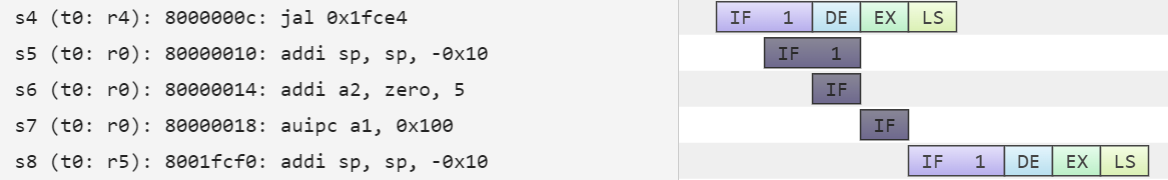
\includegraphics[width=0.96\linewidth]{design/img_flush.png}
\caption{预测错误后的流水线冲刷}
\end{figure}

\subsubsection{SoC 封装与外设映射模块}

JYDSoC 与 JYDFPGATop 分别是为 CPU 提供用于仿真和上板的运行环境平台封装，使 CPU 核心
能够方便地在仿真环境中运行，也能过渡到 FPGA 板级验证。

该平台的主要组成包括 CPUCore、IROM、DRAM、JYDPeripheralBridge，以及
LED、数码管、计数器、UART
等少量 MMIO 外设。两种平台形态的分工如下：

\begin{itemize}
\item
  \textbf{仿真版 JYDSoC：}采用便于初始化和观察的存储器实现，方便快速加载镜像、运行测试并观察外设状态。
\item
  \textbf{FPGA 版 JYDFPGATop：}保持与仿真版一致的地址空间和访问方式，并把 IROM、DRAM 和板级外设替换为实际硬件实现。
\end{itemize}

地址空间采用固定划分：IROM 基址为 \texttt{0x80000000}，DRAM 基址为
\texttt{0x80100000}，MMIO 位于 \texttt{0x80200000}
段。LED、数码管、计数器和 UART
分别占据各自的地址窗口，从而使程序、仿真环境与板级系统在地址视角下保持一致。

其中 JYDPeripheralBridge 是访存的外设桥接模块。它负责根据 CPU
发出的数据访问地址进行译码：默认请求进入 DRAM，命中其他相应窗口时则转发到
LED、SEG、CNT 或 UART（仅仿真使用） 等外设；
同时保留了模板中对计数器跨时钟 CNT 的相关寄存器的相关控制信号。通过把这些平台相关逻辑集中在桥接层，可以在不修改 CPU
核心执行语义的前提下完成仿真版与 FPGA 版平台切换。

在 FPGA 顶层实现中，IROM 和 DRAM 通过 \texttt{blk\_mem\_gen\_xxx}
黑盒接入，计数器通过板级时钟驱动的 counter IP
实现，整体保持与仿真版一致的接口习惯和访问时序。

\begin{figure}[htbp]
\centering
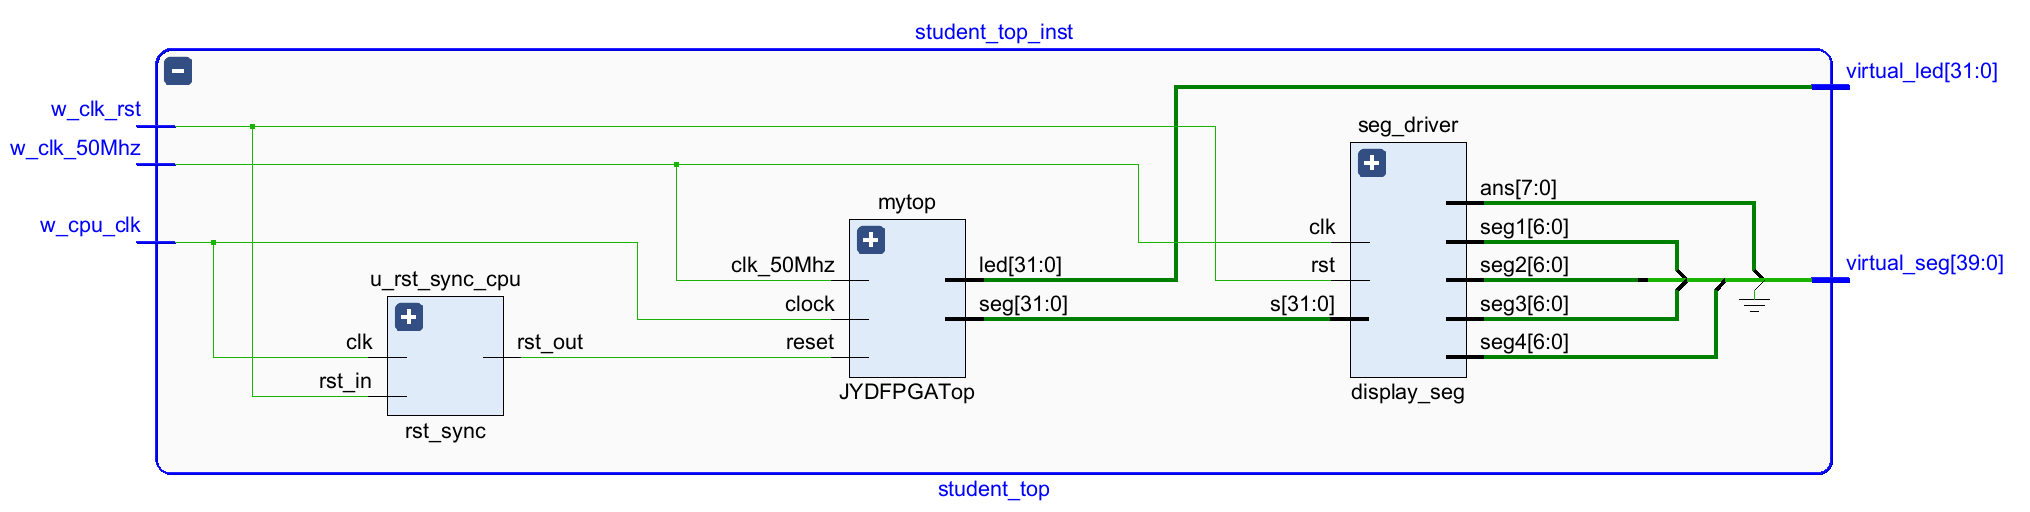
\includegraphics[width=0.96\linewidth]{design/image7.png}\\[0.6em]

\includegraphics[width=0.96\linewidth]{design/image8.png}
\caption{JYD SoC 封装与 FPGA 顶层外设映射}
\end{figure}

\subsubsection{内存接口设计}

CPU 核心内部统一采用轻量级的 SimpleBus 风格接口组织取指和数据访存。该接口既能表达只读取指，也能表达 load/store
访问，协议简单，同时又能支持未来可变延迟的外部总线桥接。

\begin{threelongtable}{@{}
  >{\raggedright\arraybackslash}p{(\linewidth - 4\tabcolsep) * \real{0.1}}
  >{\raggedright\arraybackslash}p{(\linewidth - 4\tabcolsep) * \real{0.4}}
  >{\raggedright\arraybackslash}p{(\linewidth - 4\tabcolsep) * \real{0.5}}@{}}
\caption{SimpleBus 字段说明}\\
\toprule\noalign{}
\begin{minipage}[b]{\linewidth}\raggedright
字段类别
\end{minipage} & \begin{minipage}[b]{\linewidth}\raggedright
主要信号
\end{minipage} & \begin{minipage}[b]{\linewidth}\raggedright
作用
\end{minipage} \\
\midrule\noalign{}
\endhead
\bottomrule\noalign{}
\endlastfoot
请求侧 & req\_valid、req\_ready、addr、size、wen、wdata、wmask & 表达一次读/写请求的握手、地址、访存宽度及写数据语义 \\
响应侧 & resp\_valid、rdata & 返回访存完成标志和读数据 \\
\end{threelongtable}

在核心内部，取指路径和数据路径分离：IFU 直接通过一条
SimpleBus 主口访问 IROM；数据访存则由 EXU 产生请求，经
DataMemBusCombiner 统一整理后送往 SoC 的数据口，外部的存储器结构与 CPU 解耦。

DataMemBusCombiner 在这里负责数据访存出口整理，将 EXU
发起的 load/store 请求封装到统一的数据总线形式中，并把返回结果再交给流水线后级处理。

\subsection{数据通路信号表}

\begin{threelongtable}{@{}
  >{\raggedright\arraybackslash}p{(\linewidth - 4\tabcolsep) * \real{0.1871}}
  >{\raggedright\arraybackslash}p{(\linewidth - 4\tabcolsep) * \real{0.3441}}
  >{\raggedright\arraybackslash}p{(\linewidth - 4\tabcolsep) * \real{0.4688}}@{}}
\caption{主数据通路总览}\\
\toprule\noalign{}
\begin{minipage}[b]{\linewidth}\raggedright
流向
\end{minipage} & \begin{minipage}[b]{\linewidth}\raggedright
传递内容
\end{minipage} & \begin{minipage}[b]{\linewidth}\raggedright
说明
\end{minipage} \\
\midrule\noalign{}
\endhead
\bottomrule\noalign{}
\endlastfoot
IFU -\textgreater{} IDU & inst、pc、预测信息 & 取指结果进入译码级 \\
IDU -\textgreater{} EXU & imm、src1、src2、地址预计算结果 &
译码级向执行级发送操作数与控制信息 \\
EXU -\textgreater{} LSU & 访存属性、预构造写回信息 & 访存类指令进入 LSU
时将获取读取结果 \\
LSU -\textgreater{} WBU & 访存属性、地址低位、缓存信息、写回控制 & WBU 对齐存储响应并完成最终写回 \\
EXU -\textgreater{} 访存接口 &
mem\_addr、mem\_we、mem\_wdata、mem\_wmask & 访存请求从 EXU 发出 \\
WBU -\textgreater{} GPR & rd\_we、rd\_wdata & 最终通用寄存器提交 \\
\end{threelongtable}

U类与J类指令均有写回，写回数据根据指令相关；\texttt{pc\_next} 由 EXU
确定。

\begin{threelongtable}{@{}
  >{\raggedright\arraybackslash}p{(\linewidth - 8\tabcolsep) * \real{0.0583}}
  >{\raggedright\arraybackslash}p{(\linewidth - 8\tabcolsep) * \real{0.3477}}
  >{\raggedright\arraybackslash}p{(\linewidth - 8\tabcolsep) * \real{0.2177}}
  >{\raggedright\arraybackslash}p{(\linewidth - 8\tabcolsep) * \real{0.1210}}
  >{\raggedright\arraybackslash}p{(\linewidth - 8\tabcolsep) * \real{0.2553}}@{}}
\caption{U-Type 与跳转类指令的关键数据通路}\\
\toprule\noalign{}
\begin{minipage}[b]{\linewidth}\raggedright
指令
\end{minipage} & \begin{minipage}[b]{\linewidth}\raggedright
IDU 关键数据通路
\end{minipage} & \begin{minipage}[b]{\linewidth}\raggedright
EXU 关键数据通路
\end{minipage} & \begin{minipage}[b]{\linewidth}\raggedright
写回数据
\end{minipage} & \begin{minipage}[b]{\linewidth}\raggedright
pc\_next / 控制流
\end{minipage} \\
\midrule\noalign{}
\endhead
\bottomrule\noalign{}
\endlastfoot
LUI                                    & {\ttfamily imm = immU}                            & 直接选择立即数通路                                                                               & {\ttfamily imm}        & {\ttfamily pc + 32'd4}                                                     \\
AUIPC                                  & {\ttfamily imm = immU, pc\_plus\_imm = pc + imm}  & 直接选择 \texttt{pc\_plus\_imm}                                                                  &
{\ttfamily pc\_plus\_imm}  & {\ttfamily pc + 32'd4}                \\
JAL                                    & {\ttfamily imm = immJ, pc\_plus\_imm = pc + imm}  & {\ttfamily jump = 1'b1}，跳转目标为 \texttt{pc\_plus\_imm}                                       & {\ttfamily pc + 32'd4} & {\ttfamily pc\_plus\_imm;} 若预测未命中，则 {\ttfamily pred\_wrong = 1'b1} \\
JALR                                   & {\ttfamily imm = immI, addr\_calc = src1 + imm}   & 跳转目标为
{\ttfamily \{addr\_calc[31:1], 1'b0\}} & {\ttfamily pc + 32'd4}                & {\ttfamily \{addr\_calc[31:1], 1'b0\}}；当前实现未对 JALR 做预测，故执行时总会重定向 \\
\end{threelongtable}

分支类指令：IDU 阶段统一完成：\texttt{imm = immB}、\texttt{src1 = rs1}、\texttt{src2 = rs2}、
\texttt{pc\_plus\_imm = pc + immB}；无写回；分支目标统一为
\texttt{branch\_target = pc\_plus\_imm}
（也即 \texttt{pc\_next = branch\_taken ? branch\_target : (pc + 32'd4)}）；预测错误判定方法为预测 Taken 和实际 Taken
不一致（\texttt{pred\_wrong = branch\_taken \^{} pred\_taken}）

比较运算独立于 ALU 单独完成（即未复用 ALU 计算比较）

\begin{threelongtable}{@{}
  >{\centering\arraybackslash}p{(\linewidth - 2\tabcolsep) * \real{0.1004}}
  >{\raggedright\arraybackslash}p{(\linewidth - 2\tabcolsep) * \real{0.7112}}@{}}
\caption{分支类指令的执行条件}\\
\toprule\noalign{}
\begin{minipage}[b]{\linewidth}\centering
指令
\end{minipage} & \begin{minipage}[b]{\linewidth}\raggedright
EXU 分支成立条件 branch\_taken
\end{minipage} \\
\midrule\noalign{}
\endhead
\bottomrule\noalign{}
\endlastfoot
BEQ & {\ttfamily branch\_taken = (src1 == src2)} \\
BNE & {\ttfamily branch\_taken = (src1 != src2)} \\
BLT & {\ttfamily branch\_taken = (\$signed(src1) < \$signed(src2))} \\
BGE & {\ttfamily branch\_taken = !(\$signed(src1) < \$signed(src2))} \\
BLTU & {\ttfamily branch\_taken = (src1 < src2)} \\
BGEU & {\ttfamily branch\_taken = !(src1 < src2)} \\
\end{threelongtable}

Load 类指令：IDU 阶段统一完成：\texttt{imm = immI}、\texttt{addr\_calc = src1 + imm}；EXU 阶段统一发起读请求：\texttt{mem\_addr = addr\_calc}、\texttt{mem\_we = 1'b0}；LSU
阶段统一接收：\texttt{mem\_rdata\_raw}；有写回且写回数据为处理后的访存结果；\texttt{pc\_next = pc + 32'd4}

\begin{threelongtable}{@{}
  >{\raggedright\arraybackslash}p{(\linewidth - 4\tabcolsep) * \real{0.0930}}
  >{\raggedright\arraybackslash}p{(\linewidth - 4\tabcolsep) * \real{0.2110}}
  >{\raggedright\arraybackslash}p{(\linewidth - 4\tabcolsep) * \real{0.6959}}@{}}
\caption{Load 类指令的访存与写回行为}\\
\toprule\noalign{}
\begin{minipage}[b]{\linewidth}\raggedright
指令
\end{minipage} & \begin{minipage}[b]{\linewidth}\raggedright
EXU 访存控制
\end{minipage} & \begin{minipage}[b]{\linewidth}\raggedright
WBU 写回数据
\end{minipage} \\
\midrule\noalign{}
\endhead
\bottomrule\noalign{}
\endlastfoot
LB & {\ttfamily mem\_size = 2'b00} & 从 \texttt{mem\_rdata\_raw} 中按
\texttt{mem\_addr[1:0]} 取 1 字节，并做符号扩展 \\
LH & {\ttfamily mem\_size = 2'b01} & 从 \texttt{mem\_rdata\_raw} 中按
\texttt{mem\_addr[1:0]} 取 2 字节，并做符号扩展 \\
LW & {\ttfamily mem\_size = 2'b10} & {\ttfamily load\_data = mem\_rdata\_raw} \\
LBU & {\ttfamily mem\_size = 2'b00} & 从 \texttt{mem\_rdata\_raw} 中按
\texttt{mem\_addr[1:0]} 取 1 字节，并做零扩展 \\
LHU & {\ttfamily mem\_size = 2'b01} & 从 \texttt{mem\_rdata\_raw} 中按
\texttt{mem\_addr[1:0]} 取 2 字节，并做零扩展 \\
\end{threelongtable}

注：当前实现假设访存指令的地址总是合法对齐的，不支持不对齐的字访问。

Store 类指令：IDU 阶段统一完成：\texttt{imm = immS}、\texttt{addr\_calc = src1 + imm}；EXU 阶段统一发起写请求：\texttt{mem\_addr = addr\_calc}、\texttt{mem\_we = 1'b1}；不写回 GPR；\texttt{pc\_next = pc + 32'd4}

\begin{threelongtable}{@{}
  >{\raggedright\arraybackslash}p{(\linewidth - 4\tabcolsep) * \real{0.0832}}
  >{\raggedright\arraybackslash}p{(\linewidth - 4\tabcolsep) * \real{0.1890}}
  >{\raggedright\arraybackslash}p{(\linewidth - 4\tabcolsep) * \real{0.7278}}@{}}
\caption{Store 类指令的写掩码与写数据形成方式}\\
\toprule\noalign{}
\begin{minipage}[b]{\linewidth}\raggedright
指令
\end{minipage} & \begin{minipage}[b]{\linewidth}\raggedright
EXU 访存控制
\end{minipage} & \begin{minipage}[b]{\linewidth}\raggedright
写掩码与写数据形成方式
\end{minipage} \\
\midrule\noalign{}
\endhead
\bottomrule\noalign{}
\endlastfoot
SB & {\ttfamily mem\_size = 2'b00} & \texttt{mem\_wmask} 为 1 字节 one-hot
掩码；\texttt{mem\_wdata} 将 \texttt{src2[7:0]} 放到目标字节位置 \\
SH & {\ttfamily mem\_size = 2'b01} & \texttt{mem\_wmask} 为 2
字节掩码；\texttt{mem\_wdata} 将 \texttt{src2[15:0]} 放到目标半字位置 \\
SW & {\ttfamily mem\_size = 2'b10} & {\ttfamily mem\_wmask = 4'b1111; mem\_wdata = src2} \\
\end{threelongtable}


I-Type 算术/逻辑指令共同特点：IDU 阶段统一完成：\texttt{imm = immI}；EXU ALU 使用 \texttt{src1 = rs1}、
\texttt{src2 = imm}；有写回且写回数据 \texttt{rd\_wdata = alu\_y}；\texttt{pc\_next = pc + 32'd4}

\begin{threelongtable}{@{}
  >{\centering\arraybackslash}p{(\linewidth - 2\tabcolsep) * \real{0.1004}}
  >{\raggedright\arraybackslash}p{(\linewidth - 2\tabcolsep) * \real{0.7712}}@{}}
\caption{I-Type 算术/逻辑指令的 EXU 运算}\\
\toprule\noalign{}
\begin{minipage}[b]{\linewidth}\centering
\textbf{指令}
\end{minipage} & \begin{minipage}[b]{\linewidth}\centering
\textbf{EXU 运算}
\end{minipage} \\
\midrule\noalign{}
\endhead
\bottomrule\noalign{}
\endlastfoot
ADDI & {\ttfamily alu\_y = src1 + src2} \\
SLTI & {\ttfamily alu\_y = (\$signed(src1) < \$signed(src2)) ? 32'd1 : 32'd0} \\
SLTIU & {\ttfamily alu\_y = (src1 < src2) ? 32'd1 : 32'd0} \\
XORI & {\ttfamily alu\_y = src1 \^{} src2} \\
ORI & {\ttfamily alu\_y = src1 | src2} \\
ANDI & {\ttfamily alu\_y = src1 \& src2} \\
SLLI & {\ttfamily alu\_y = src1 << src2[4:0]} \\
SRLI & {\ttfamily alu\_y = src1 >> src2[4:0]} \\
SRAI & {\ttfamily alu\_y = \$signed(src1) >>> src2[4:0]} \\
\end{threelongtable}

R-Type 算术/逻辑指令共同特点：EXU ALU 使用：\texttt{src1 = rs1}、\texttt{src2 = rs2}；有写回且写回数据 \texttt{rd\_wdata = alu\_y}；\texttt{pc\_next = pc + 32'd4}

\begin{threelongtable}{@{}
  >{\centering\arraybackslash}p{(\linewidth - 2\tabcolsep) * \real{0.1138}}
  >{\raggedright\arraybackslash}p{(\linewidth - 2\tabcolsep) * \real{0.7443}}@{}}
\caption{R-Type 算术/逻辑指令的 EXU 运算}\\
\toprule\noalign{}
\begin{minipage}[b]{\linewidth}\centering
\textbf{指令}
\end{minipage} & \begin{minipage}[b]{\linewidth}\centering
\textbf{EXU 运算}
\end{minipage} \\
\midrule\noalign{}
\endhead
\bottomrule\noalign{}
\endlastfoot
ADD & {\ttfamily alu\_y = src1 + src2} \\
SUB & {\ttfamily alu\_y = src1 - src2} \\
SLL & {\ttfamily alu\_y = src1 << src2[4:0]} \\
SLT & {\ttfamily alu\_y = (\$signed(src1) < \$signed(src2)) ? 32'd1 : 32'd0} \\
SLTU & {\ttfamily alu\_y = (src1 < src2) ? 32'd1 : 32'd0} \\
XOR & {\ttfamily alu\_y = src1 \^{} src2} \\
SRL & {\ttfamily alu\_y = src1 >> src2[4:0]} \\
SRA & {\ttfamily alu\_y = \$signed(src1) >>> src2[4:0]} \\
OR & {\ttfamily alu\_y = src1 | src2} \\
AND & {\ttfamily alu\_y = src1 \& src2} \\
\end{threelongtable}

\subsection{控制器设计}

\subsubsection{控制信号表}

\begin{threelongtable}{@{}
  >{\raggedright\arraybackslash}p{(\linewidth - 12\tabcolsep) * \real{0.1389}}
  >{\raggedright\arraybackslash}p{(\linewidth - 12\tabcolsep) * \real{0.1351}}
  >{\raggedright\arraybackslash}p{(\linewidth - 12\tabcolsep) * \real{0.1372}}
  >{\raggedright\arraybackslash}p{(\linewidth - 12\tabcolsep) * \real{0.1380}}
  >{\raggedright\arraybackslash}p{(\linewidth - 12\tabcolsep) * \real{0.1534}}
  >{\raggedright\arraybackslash}p{(\linewidth - 12\tabcolsep) * \real{0.1655}}
  >{\raggedright\arraybackslash}p{(\linewidth - 12\tabcolsep) * \real{0.1318}}@{}}
\caption{控制信号表}\\
\toprule\noalign{}
\begin{minipage}[b]{\linewidth}\centering
\textbf{指令类别}
\end{minipage} & \begin{minipage}[b]{\linewidth}\centering
\textbf{rdWrEn}
\end{minipage} & \begin{minipage}[b]{\linewidth}\centering
\textbf{memRead}
\end{minipage} & \begin{minipage}[b]{\linewidth}\centering
\textbf{memWrite}
\end{minipage} & \begin{minipage}[b]{\linewidth}\centering
\textbf{wbSel}
\end{minipage} & \begin{minipage}[b]{\linewidth}\centering
\textbf{pcSel}
\end{minipage} & \begin{minipage}[b]{\linewidth}\centering
\textbf{csrEn}
\end{minipage} \\
\midrule\noalign{}
\endhead
\bottomrule\noalign{}
\endlastfoot
寄存器运算 & 1 & 0 & 0 & ALU & PC+4 & 0 \\
立即数运算 & 1 & 0 & 0 & ALU & PC+4 & 0 \\
Load & 1 & 1 & 0 & LOAD & PC+4 & 0 \\
Store & 0 & 0 & 1 & - & PC+4 & 0 \\
Branch & 0 & 0 & 0 & - & BRANCH & 0 \\
JAL/JALR & 1 & 0 & 0 & SNPC & JUMP & 0 \\
LUI/AUIPC & 1 & 0 & 0 & IMM/PCIMM & PC+4 & 0 \\
CSR/异常 & 按指令 & 0 & 0 & CSR & CSR\_TARGET & 按指令 \\
\end{threelongtable}

\subsubsection{控制器设计说明}

控制器采用``粗粒度类型译码 + 细粒度字段判别''的方式实现。首先，IDU 中的
InstInfoDecoder 按 opcode 将指令归入格式与类型集合；随后，EXU 再结合
funct3、funct7 完成算术、访存宽度、分支条件和 CSR
操作的具体判定。这种分层控制方式将组合逻辑拆散到不同阶段，有利于工程维护与时序收敛。

\section{CPU 性能优化设计}

围绕竞业达 FPGA 平台上的关键路径，主要的优化思路包括：
把存储器更换为时序性能更优的 BRAM 同时尽可能隐藏访存延迟的影响；
把原本集中在 EXU/LSU 等复杂模块上的计算适当前移或后移，从而降低综合与布局的时序压力；
通过仿真分析和性能评估工具的反馈优化架构设计。

\subsection{使用带有输出寄存器的 BRAM}

默认模板的 IROM 和 DRAM 是同周期异步读写的 Distributed Memory 结构，逻辑延迟较大，难以满足高频率时序要求。
因此我们使用 FPGA 上更适合高频的 BRAM 结构替换原有存储器实现。IROM 保持固定一周期读延迟，
并由 IFU 连续取指状态机隐藏。数据 BRAM 在板卡上的物理位置相对固定，BRAM 输出到流水线寄存器
之间的布线距离较长；实际综合和布局布线表明，即使继续压缩 LSU 组合逻辑，也很难让一周期读路径
稳定满足 280 MHz 要求。综合权衡工作频率、访存停顿和实现稳定性后，决赛版本为 DRAM 启用输出寄存器，
使读请求在两拍后产生 \texttt{resp\_valid}。该寄存器切断 BRAM 输出长布线路径，流水线再通过
提前发请求、WBU 后移整理和 D-cache 命中旁路降低额外读延迟的性能影响。

\subsection{前端控制流优化}

前端优化首先体现在 IFU 的连续取指能力上。
因为换用了固定一周期返回的 BRAM 作为IROM，每条指令的取指过程都将固定多出一拍的等待时间。
如果仍然按照正常等待取指响应完成后再发出下一条指令的取指请求，则会导致前端频繁停顿，严重影响性能。
一种方法是使用 ICache 结构隐藏取指延迟，但我们注意到可以利用 IFU 内部的状态机设计，在得到响应
的同周期就立刻发出下一条指令的取指请求，从而在顺序指令流的情况下\textbf{把 BRAM 的一拍延迟隐藏掉}。
当上一条取指响应返回、后级也在同周期接收成功时，IFU
可以立刻接入新的 PC 并尝试发起下一次请求，因此对顺序指令流而言，BRAM
的一拍延迟在前端大部分时候可以被连续流动隐藏掉。

\begin{figure}[htbp]
\centering
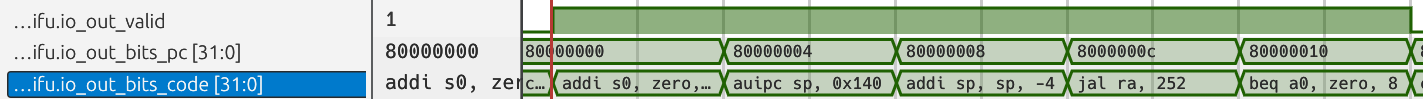
\includegraphics[width=1\linewidth]{design/imaged.png}\\[0.5em]
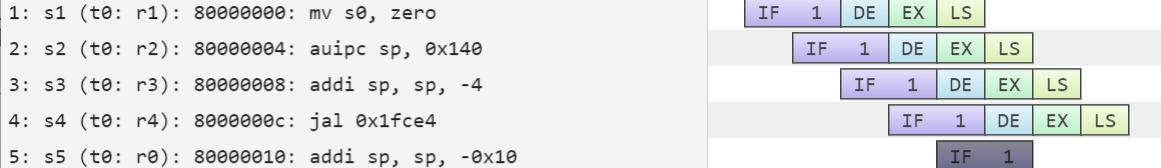
\includegraphics[width=1\linewidth]{design/imagee.png}
\caption{BRAM 一周期延迟隐藏的取指}
\end{figure}

控制流预测部分采用简单且利于时序的静态方案。当前分支目标缓存采用
16 项 BTB 表项，并配合 BTFN 策略使用：当 BTB 命中后，只有 JAL
或向后分支会被预测为 taken，其中``向后''直接由分支立即数的符号位表示，在 EXU 中检测到分支时更新
，而不额外引入更复杂的历史状态。
后端校验时也\textbf{不需要条件分支比较完整预测目标与真实目标，只需要检查预测方向是否一致}；
因为对条件分支而言，方向一旦判断错误就必然需要重定向，而方向正确时目标地址已由
\texttt{PC+imm} 唯一确定。这样既减少了比较逻辑，也避免把无必要的目标比对放进关键路径。

\begin{table}[htbp]
\centering
\caption{不同 BTB 表项数下的预测命中率对比}
\scriptsize
\begin{tabular}{ccccccc}
\toprule
\textbf{BTB 表项数} & 2 & 4 & 8 & 16 & 32 & 64 \\
\midrule
\textbf{预测准确率} & 33.89\% & 48.64\% & 63.02\% & 65.86\% & 66.53\% & 66.64\% \\
\bottomrule
\end{tabular}
\end{table}

从仿真数据看，BTB 表项数从 2 项增加到 4 项时，命中率提升
14.75 个百分点；从 4 项增加到 8 项时，继续提升 14.38
个百分点，说明较小 BTB 容量下冲突缺失仍然是前端控制流预测的主要损失来源。
但当表项数超过 8 项后，收益迅速收敛：16 项相比 8 项只提升
2.84 个百分点，32 项相比 16 项只提升 0.67 个百分点，64
项相比 32 项仅提升 0.11 个百分点。也就是说，在当前测试负载下，
8 项 BTB 已经覆盖了大部分高频跳转目标，继续增大表项数主要只能减少少量低频冲突。

初赛实现据此选择 8 项 BTB；决赛阶段在进一步分析冲突缺失后将容量提升为 16 项，获得表中
2.84 个百分点的额外准确率。进一步的时序实验还发现，直接映射 BTB 增加表项数会增加 index 位数，
却同时减少 tag 位数；后者会缩短 tag 等值比较器及其后续命中判定逻辑。在当前实现中，tag 比较的
时序压力与命中后的 target Mux 选择相当，部分实现结果中甚至更大，因此从 8 项增加到 16 项并未
像单纯扩大阵列那样明显增加关键路径压力，实际时序代价很小。

决赛版本还把 PC、tag 和 target 缩减为 \texttt{[16:2]} 的 15 位字地址表示，进一步缩短 tag
比较和目标 Mux。由此，16 项配置既减少冲突缺失，也利用更短 tag 抵消额外索引与选择开销，最终在
预测覆盖率、资源与 280 MHz 时序约束之间取得折中。

\subsection{译码级前移与阻塞削减}

为了减轻 EXU 的组合深度，IDU
并不只负责翻译 opcode，而是在译码阶段就完成一部分后续高频使用的预计算。首先，指令格式和类型在
IDU 中以\textbf{独热码}形式生成，后续各级只需按位判断是否属于 load、store、branch、jal
等类别，不必重复构造一组完整译码条件。其次，\texttt{PC+imm}、\texttt{rs1+imm}
等\textbf{结果也在 IDU 中提前形成}，其中前者直接服务于分支和 JAL
目标地址，后者直接服务于 load/store/JALR 的地址生成。这样可以把最常用的加法运算从
EXU 中拆出去，\textbf{缩短 EXU 上的组合链路}。

对 \texttt{rs1+imm} 的相关处理并未复用完整的普通 EXU 旁路网络。性能统计表明，只有
load、store 和 JALR 需要该结果，而它们紧邻依赖上一条指令的情况较少；即使发生，生产者绝大多数
也是加法类指令。为避免把完整 ALU 结果选择 Mux 拉入地址生成关键路径，IDU 对上一拍 EXU 只接收
专用的加法结果前递；对 LUI、AUIPC、JAL/JALR 和 CSR 等不需要等待通用 ALU 计算即可确定的结果，
则使用预先形成的写回值，并在后续流水级按有效性参与地址基值选择。其他尚未得到结果的相关仍通过
\texttt{dataValid} 触发停顿，从而以很小的覆盖损失换取更短、更稳定的地址生成路径。

IDU 同时提前选择一部分 EXU 所需的写回候选：LUI 选择 U 型立即数，AUIPC 选择
\texttt{pc+imm}，JAL/JALR 选择顺序下一 PC，系统指令选择 CSR 旧值。EXU 只需在这些预选结果与
普通 ALU、乘除法结果之间作较浅的最终选择，避免在执行级重复放置按指令类型展开的宽 Mux。

IDU 还提前完成了两类会显著影响后端关键路径的工作。其一是 CSR
读取：当前指令需要访问的 CSR 在译码阶段就发起单读端口访问，并把读出值直接作为
EXU 输入，\textbf{避免在 EXU 中再使用 CSR 读后 Mux 路径}。其二是异常与返回类控制流的下一跳选择：\texttt{ecall}
对应的 \texttt{mtvec}、\texttt{mret} 对应的 \textbf{\texttt{mepc}
在 IDU 中预先选成静态下一跳，减轻 EXU
控制流选择压力}。与此同时，对于本来就不需要第二源寄存器的指令，IDU 会直接把
\texttt{rs2} 置为 0，使旁路网络\textbf{不对无效的 \texttt{rs2}
地址进行冲突匹配}，从而减少不必要的阻塞与停顿判定。

\subsection{执行与访存关键路径压缩}

执行级的核心优化是尽可能提早发起访存，同时把不必要留在关键路径上的整理逻辑移走。对
load/store 指令，EXU 直接使用 IDU 已经算好的 \texttt{rs1+imm}
作为目标地址，并在本级构造访存请求。当前 DRAM 是带输出寄存器的两周期读存储器，因此 LSU
先保存访存属性和写回元信息，WBU 再与第二拍到达的 \texttt{resp\_valid} 对齐并完成提交。
请求仍在 EXU 尽早发出，避免把地址生成额外推迟一拍。对于 store，字节写、半字写的掩码生成以及写数据对齐都\textbf{通过
Mux 组合网络完成，而不是使用变量位移指令}实现。这样做虽然在功能上等价，但综合后通常能得到更可控的硬件结构，
\textbf{避免将可变移位器引入访存通路}。

与之对应，LSU 的职责被刻意压缩为``传递访存元信息并提供缓存旁路''，而不是在本级接收并整理
DRAM 响应。当前设计把地址低位、\texttt{func3}、缓存命中信息和写回控制传给 WBU；第二周期的
原始 32 位 \texttt{memResp} 直接到达 WBU，再由 WBU 完成字节/半字抽取以及符号扩展、零扩展。
这样安排的原因是：在板级实现中，\textbf{BRAM
位置固定且输出布线延迟较高}，一周期读方案难以在 280 MHz 下稳定收敛；即使采用两周期读，若在 LSU
立刻叠加位扩展和结果选择逻辑，会进一步压缩时序余量。把这些工作后\textbf{移到 WBU
后，LSU 关键路径更短}，而写回级本身又具备更充足的组合预算，整体上更有利于频率与布线收敛。

虽然会导致旁路网络在 load-use 情况下多停顿一拍，但评估认为主频提升带来的每秒指令吞吐率增益
可以弥补这一影响；该变化并不等同于 IPC 提升。

\subsection{数据缓存与重复访存优化}

两周期 DRAM 有利于时序，但会放大频繁重复读取的性能损失。为此，数据侧增加 2 KiB、512 行、
每行 32 位的直接映射 D-cache，仅覆盖最常见的 DRAM 对齐 \texttt{LW}。地址索引直接选择表项，
tag 与 valid 判定命中；命中数据在 LSU 阶段提前参与旁路，miss 则保持原有 DRAM 请求与 WBU
回填流程。tag/valid 阵列使用 512$\times$8 分布式存储器，查询地址通过异步读端口在同一周期得到
tag 表项并完成命中比较；数据阵列则使用同步读 BRAM。这样 EXU 发出请求时已经形成命中信息，LSU
只需按已寄存的命中结果取得缓存数据，避免在下一级把 tag 读取、比较以及“缓存/普通数据”宽 Mux
串接为一条长组合路径。

这里的 epoch 是一个 8 位全局 store 版本计数器：每次对可缓存 DRAM 地址执行 store 并使缓存行
失效时，计数器加一；load 在 EXU 发出时把当前 epoch 快照随访存元信息送入 LSU/WBU。对于 miss
返回，WBU 只有在“快照 epoch 等于当前 epoch”时才允许回填。这意味着该 load 之后没有更年轻的
store 发生；若两者不同，即使 DRAM 旧读响应随后到达，也只用于本条 load 的体系结构写回，不再写入
D-cache，从而避免年轻 store 的失效被较老 load 的迟到回填覆盖。DCache 内部还规定同周期
invalidate 的优先级高于 WBU update，进一步保证 store 一致性。

\begin{figure}[htbp]
\centering
\resizebox{0.94\linewidth}{!}{%
\begin{tikzpicture}[node distance=0.8cm and 1.2cm,
  block/.style={draw,rounded corners,align=center,minimum height=0.85cm,fill=blue!5},
  decision/.style={draw,diamond,aspect=2,align=center,fill=orange!5},
  arrow/.style={-Stealth,thick}]
  \node[block] (req) {EXU 对齐 LW 请求};
  \node[decision,right=of req] (hit) {D-cache 命中？};
  \node[block,above right=of hit] (fwd) {LSU 提前旁路};
  \node[block,below right=of hit] (dram) {等待两周期 DRAM};
  \node[block,right=of dram] (fill) {WBU 校验 epoch\\并回填};
  \draw[arrow] (req)--(hit);
  \draw[arrow] (hit)--node[above left]{是}(fwd);
  \draw[arrow] (hit)--node[below left]{否}(dram);
  \draw[arrow] (dram)--(fill);
\end{tikzpicture}
}
\caption{D-cache 命中旁路与未命中回填流程}
\end{figure}

\subsection{实现时序与性能结果}

决赛版本在 Vivado 2024.2 下以 280 MHz 完成综合、布局布线，最差时序裕量 WNS 为
\textbf{+0.050 ns}，时序报告无 setup 违例。与初赛 250 MHz 版本相比，三组官方性能程序均缩短：

\begin{table}[htbp]
\centering
\caption{初赛与分赛区决赛性能对比}
\begin{tabular}{lrrr}
\toprule
测试程序 & 初赛时间/s & 决赛时间/s & 时间降低 \\
\midrule
\texttt{src0} & 8.706 & 7.101 & 18.4\% \\
\texttt{src1} & 9.803 & 7.047 & 28.1\% \\
\texttt{src2} & 10.592 & 9.233 & 12.8\% \\
\bottomrule
\end{tabular}
\end{table}

三组平均运行时间由 9.700 s 降至 7.794 s，平均降低约 19.7\%。新的 M 扩展测评程序中，
\texttt{withoutMext} 用时 3.890 s，\texttt{withMext} 用时 2.020 s；启用硬件乘除法后时间降低
48.1\%，等效加速约 1.93 倍。以上结果同时体现了频率提升、数据通路优化和硬件 M 扩展的综合收益。

\section{CPU 特色功能设计}

本章重点说明 CPU 内核自身在基础 RV32I 指令之外补充实现的功能。这些功能一方面用于支撑更完整的软件运行环境，
另一方面也使 CPUCore 能够在不同 SoC 封装中复用。

\subsection{CSR 与机器模式控制流支持}

CPU 内核实现了面向机器模式运行环境的 CSR 子集，支持
\texttt{mstatus}、\texttt{mtvec}、\texttt{mepc}、\texttt{mcause}、
\texttt{mcycle}、\texttt{mcycleh}、\texttt{mvendorid} 和 \texttt{marchid}
等寄存器，并实现了 \texttt{CSRRW}、\texttt{CSRRS}、\texttt{CSRRC} 及其立即数形式
\texttt{CSRRWI}、\texttt{CSRRSI}、\texttt{CSRRCI}，同时实现 \texttt{ECALL} 与
\texttt{MRET} 相关机器态控制流。当前功能为后续适配 RT-Thread 提供基础；由于尚未实现完整的
异常与中断体系，本文不对 RT-Thread 的完整运行能力作保证。

CSR 访问被拆分到流水线中处理：IDU 在译码阶段根据指令高 12 位发起 CSR
读取，并提前选择 \texttt{ecall} 对应的 \texttt{mtvec} 或 \texttt{mret}
对应的 \texttt{mepc} 作为静态跳转目标；EXU 再根据指令类型生成 CSR
写回使能、写地址和写数据；WBU 在最终提交点统一更新 CSR 寄存器堆。这样既保持了顺序提交语义，也避免在
EXU 中再叠加较长的 CSR 读后选择路径。

\subsection{可桥接 AXI4 的存储访问接口}

CPUCore 内部的取指和访存接口使用两路 SimpleBus：IFU 负责指令读取，LSU/数据访存通路负责
load/store 请求。为了让 CPU 内核能够接入更通用的 SoC 总线，工程中实现了
\texttt{DualSimpleBusToAXI4} 桥接模块，将 IFU 与 LSU 两路 SimpleBus
请求汇聚为一路 AXI4 master 接口。
该桥接模块在空闲状态下优先接受 LSU 请求，避免数据访存长期被取指流阻塞；读请求通过
AXI4 \texttt{AR/R} 通道完成，写请求通过 \texttt{AW/W/B} 通道完成，并用状态机记录
\texttt{AW} 与 \texttt{W} 两个通道是否已经握手。当前竞业达 JYD FPGA 顶层为了适配板级
IROM、DRAM 和外设桥，没有启用 AXI4 版本的顶层接口；但 CPU 顶层和桥接模块已经保留，
便于后续切换到 AXI4 内存、AXI4 交叉开关或其他 SoC 验证环境。

\newpage

\clearpage
\section{验证与测评体系}

\subsection{验证平台说明}

本项目最终验证平台为竞业达 FPGA 数字孪生平台，对应开发板核心器件为 Xilinx Kintex-7 XC7K325T-2FFG900。板端可观察资源主要包括 LED 阵列、八位数码管以及平台状态指示区，能够满足本项目对程序运行结果可视化展示的需要。

\subsubsection{下载/烧录工具版本}

bitstream 生成阶段使用 Vivado 2024；远程下载与板级观察阶段使用竞业达数字孪生平台配套的自动烧录工具。工程完成综合、实现和比特流生成后，通过平台加载设备、选择 bit 文件并执行远程烧录。

\subsubsection{上电与平台显示验证说明}

本项目的板级外设连接基于竞业达官方提供的 FPGA 模板完成，LED、数码管和 UART 等接口均已在模板顶层中预先接好。本项目在此基础上完成 CPU 顶层与板级显示逻辑的对接，其中 UART 主要用于与孪生数字平台进行通信，并非本次上板验证中面向用户的主要交互输出通道；本次验证结果主要通过平台运行状态、LED 阵列显示和数码管显示进行判断。

具体实现上，本项目将 LED 与数码管显示值作为设备寄存器相关输出接入自定义 Top 顶层，其中数码管显示值通过模板提供的显示驱动模块转换为可直接驱动数码管的控制信号，再与 LED 显示信息一并送入板级控制路径，由孪生数字平台完成状态同步与显示。

在实际测试过程中，完成 bitstream 烧录并打开数字孪生平台后，若平台运行状态显示正常，且 LED、数码管显示结果与测试程序预期一致，则判定该测试用例通过。

\subsection{测试用例说明}

\subsubsection{指令程序例程}

本次上板验证采用官方工程提供的 \texttt{src0}、\texttt{src1}、\texttt{src2}，以及新测试程序
\texttt{withoutMext}、\texttt{withMext}。五组程序均已完成比特流生成，
并在竞业达数字孪生平台上完成烧录与运行验证。

\subsubsection{上板运行流程说明}

\begin{enumerate}[label=\arabic*）]
  \item 在 Vivado 2024.2 中打开工程，完成综合、实现并生成 bitstream。
  \item 配置孪生平台网络连接环境，启动数字孪生平台并加载可用设备。
  \item 在烧录界面中选择生成的 bit 文件，执行远程烧录。
  \item 烧录成功后打开孪生平台界面，观察``运行状态''、``数据运行正常''、``串口运行正常''等状态提示。
  \item 记录 LED 阵列和八位数码管显示结果，并与测试用例预期进行比对。
  \item 依次完成五组程序的上板验证。
\end{enumerate}

\subsection{仿真平台介绍}

\subsubsection{仿真工具}

本项目中使用的仿真工具分为两类：一类为 Vivado Simulation 自带的仿真工具，用于进行包含数码管、LED、BRAM 等板级外设后的板级行为正确性仿真和时序后仿。另一类为基于 Verilator 和 C/C++ 搭建的高性能行为仿真平台，便于快速仿真、实现自定义需求功能。

\subsubsection{测试环境说明}

\paragraph{Vivado 仿真测试平台}

仿真环境 Vivado 2024.2，Windows 本地工程，使用 Run Behavioral Simulation 观察波形，检查是否向数码管等外设写入预期正确值。

\begin{figure}[H]
  \centering
  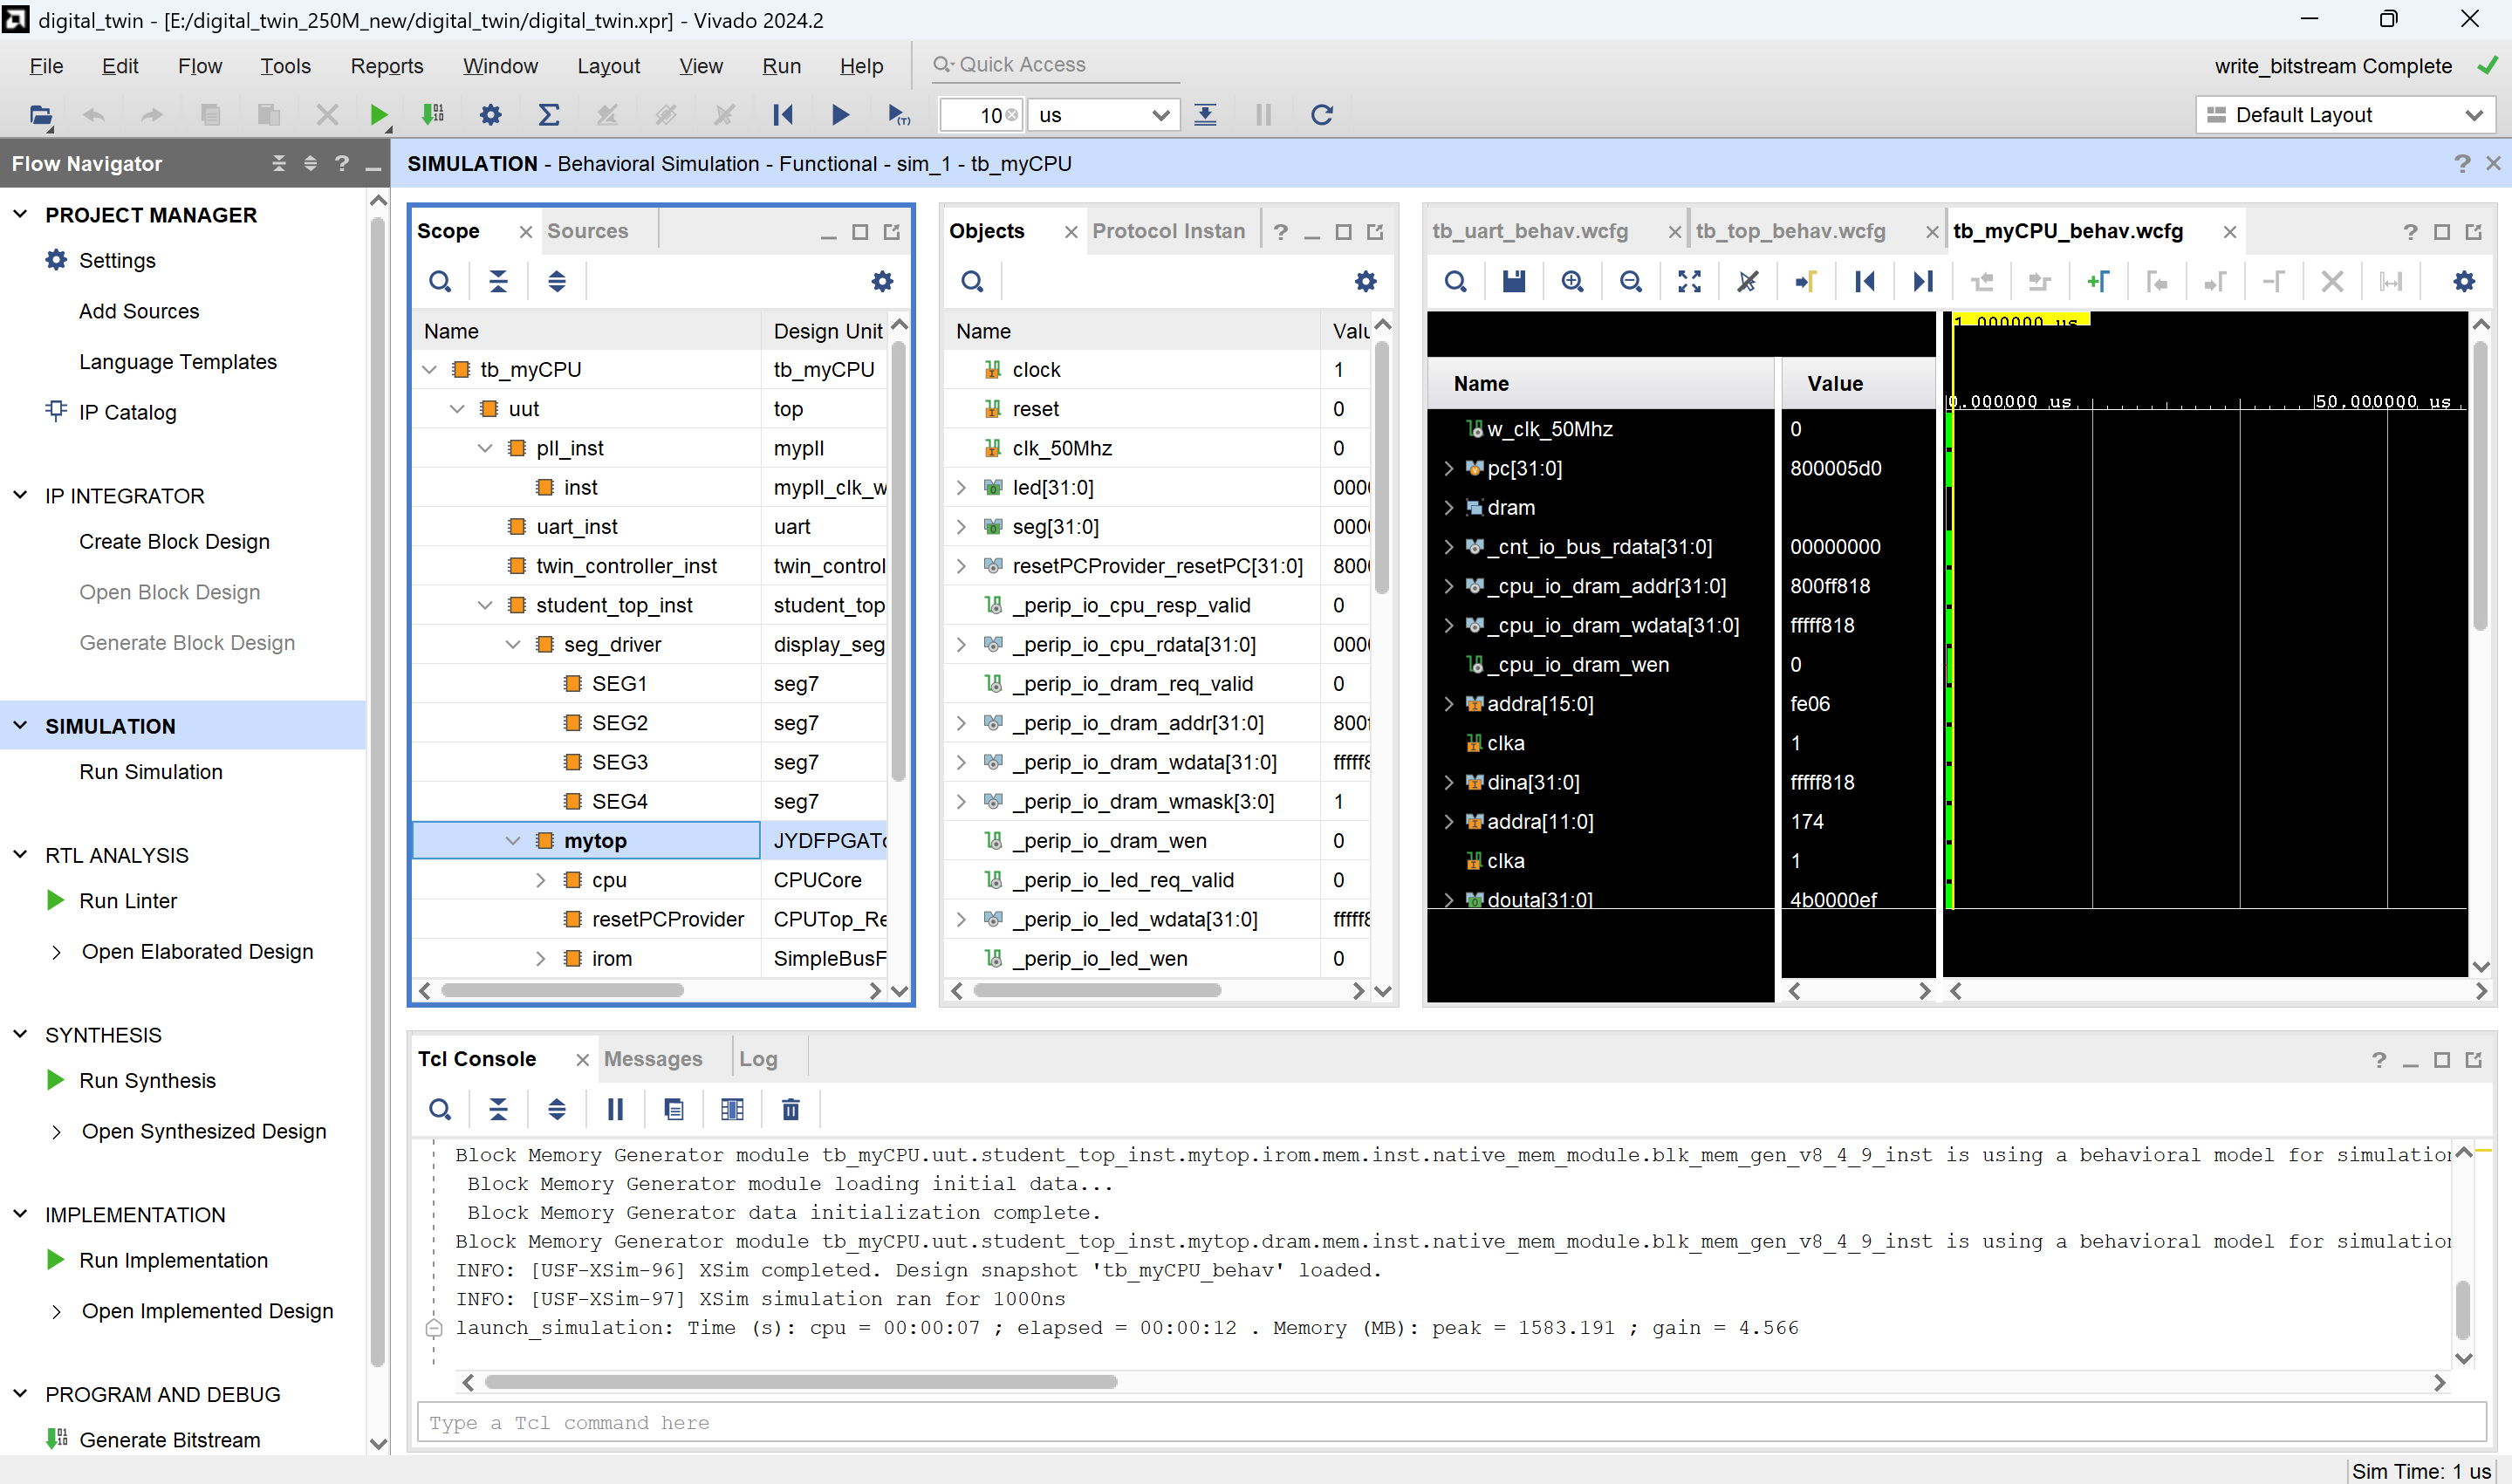
\includegraphics[width=\linewidth]{verify/image8.png}
  \caption{Vivado 仿真工程界面}
\end{figure}

\paragraph{Verilator 仿真测试平台}

实现了性能统计、差分测试、行为踪迹、流水线日志、接入 GitHub Actions 自动化集成测试。测试仿真日志中的 Perf Counters Report 统计了周期数、指令数、IPC、CPI、分支预测准确率和 RAW stall 等性能指标。

项目 CPU 通过直接编程接口（DPI-C）方法实现了 EBREAK 的仿真时支持，通过为测试程序提供基础运行库使其停机（halt）后执行 EBREAK，触发仿真程序检查 a0 寄存器作为 main 函数返回值是否为 0 来判定测试程序是否正确运行。并使用了软件 RISC-V 模拟器\footnote{参考了\href{https://ysyx.oscc.cc/docs/}{一生一芯项目}对 CPU 测试的资料，软件模拟器 NEMU 在其讲义指导下独立实现完成。}，作为差分测试的参考执行。

同时使用 DPI-C 方法在软件层面模拟了竞业达板卡的 LED 和 SEG 外设，使得可以运行官方 coe 文件，拥有相对一致的外设行为。

并参考一生一芯项目 B 线 CI 测试\footnote{因 B 阶段 CI 测试仍处于内测阶段，根据相关要求，暂不便提供参考链接。}，
基于 GitHub Actions 搭建了自动化正确性测试、性能测试和 Vivado 执行流程。本次分赛区决赛版本
对应的 CI 记录为 \href{https://github.com/HanPiM/jyd/actions/runs/29162587063}{Actions run 29162587063}，
其中用户提供的 \texttt{withMext-v2} 任务记录为
\href{https://github.com/HanPiM/jyd/actions/runs/29162587063/job/86570180985}{job 86570180985}；
被测提交为 \texttt{585ebc2b7f41ea65fb4c6536f9a6747171495258}。

\begin{figure}[H]
  \centering
  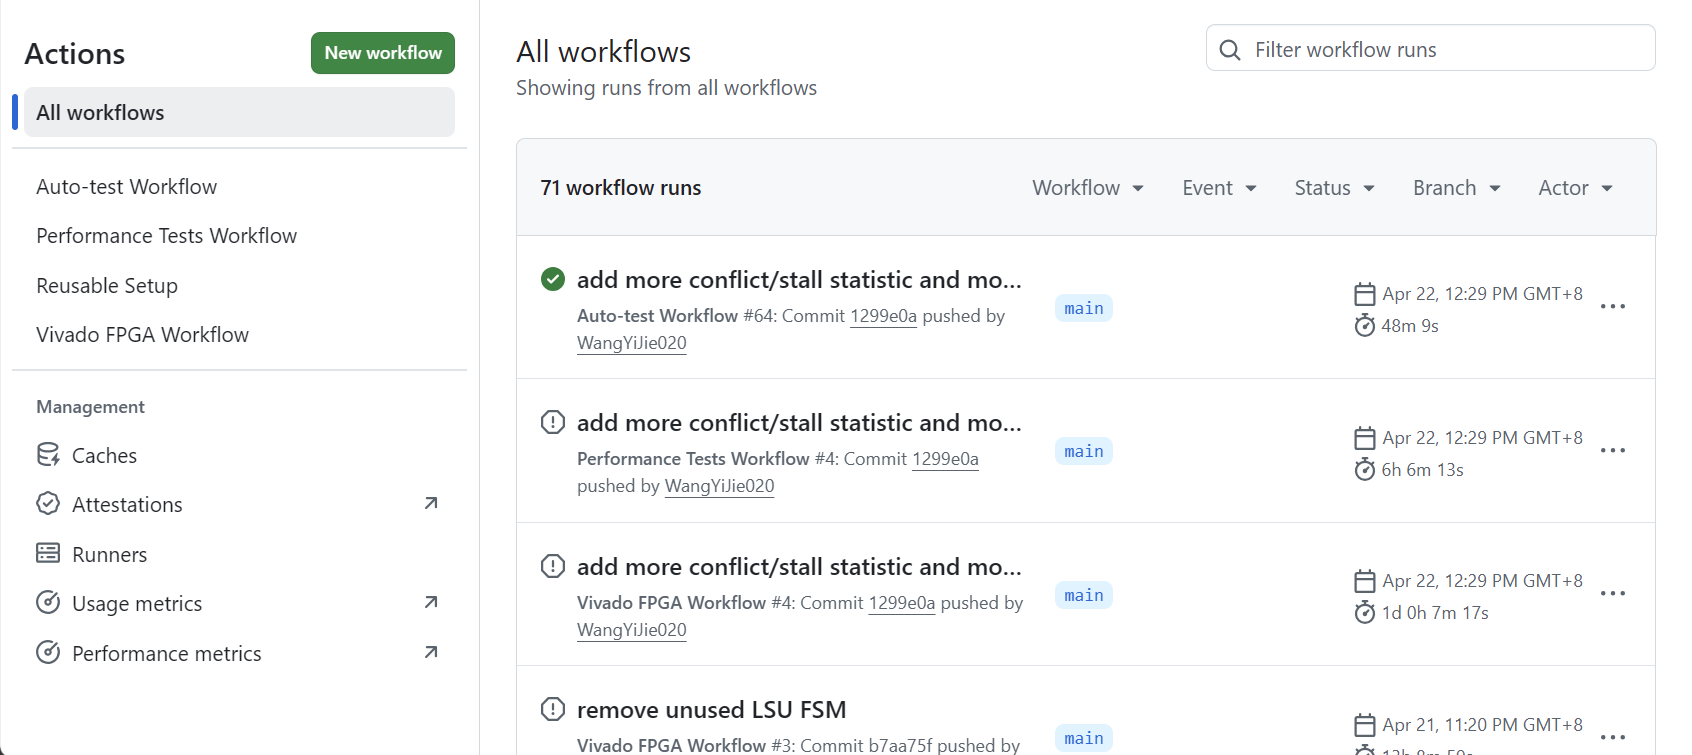
\includegraphics[width=\linewidth]{verify/image9.png}
  \caption{GitHub Actions 界面}
\end{figure}

每次提交新代码后会自动触发系列测试运行，具体测试流程：对于 C 代码测试程序，使用 riscv64-linux-gnu 工具链编译成二进制文件、使用 riscv64-linux-gnu-objcopy 提取 .text 段和 .data 段作为 IROM 和 DRAM 初始化数据、执行仿真直到 EBREAK、检查正确性；对于 coe 文件，使用脚本转换为二进制文件后同上流程进行仿真。

\subsection{RV32I CPU 测试}

\subsubsection{RV32I指令集测试}

针对 RV32I 指令集的测试，采用了单指令单元测试和小规模程序测试的方法验证。测试项目选用了南京大学相关实验项目提供的基于裸机运行环境的开源 RISC-V 测试集。

\begin{figure}[H]
  \centering
  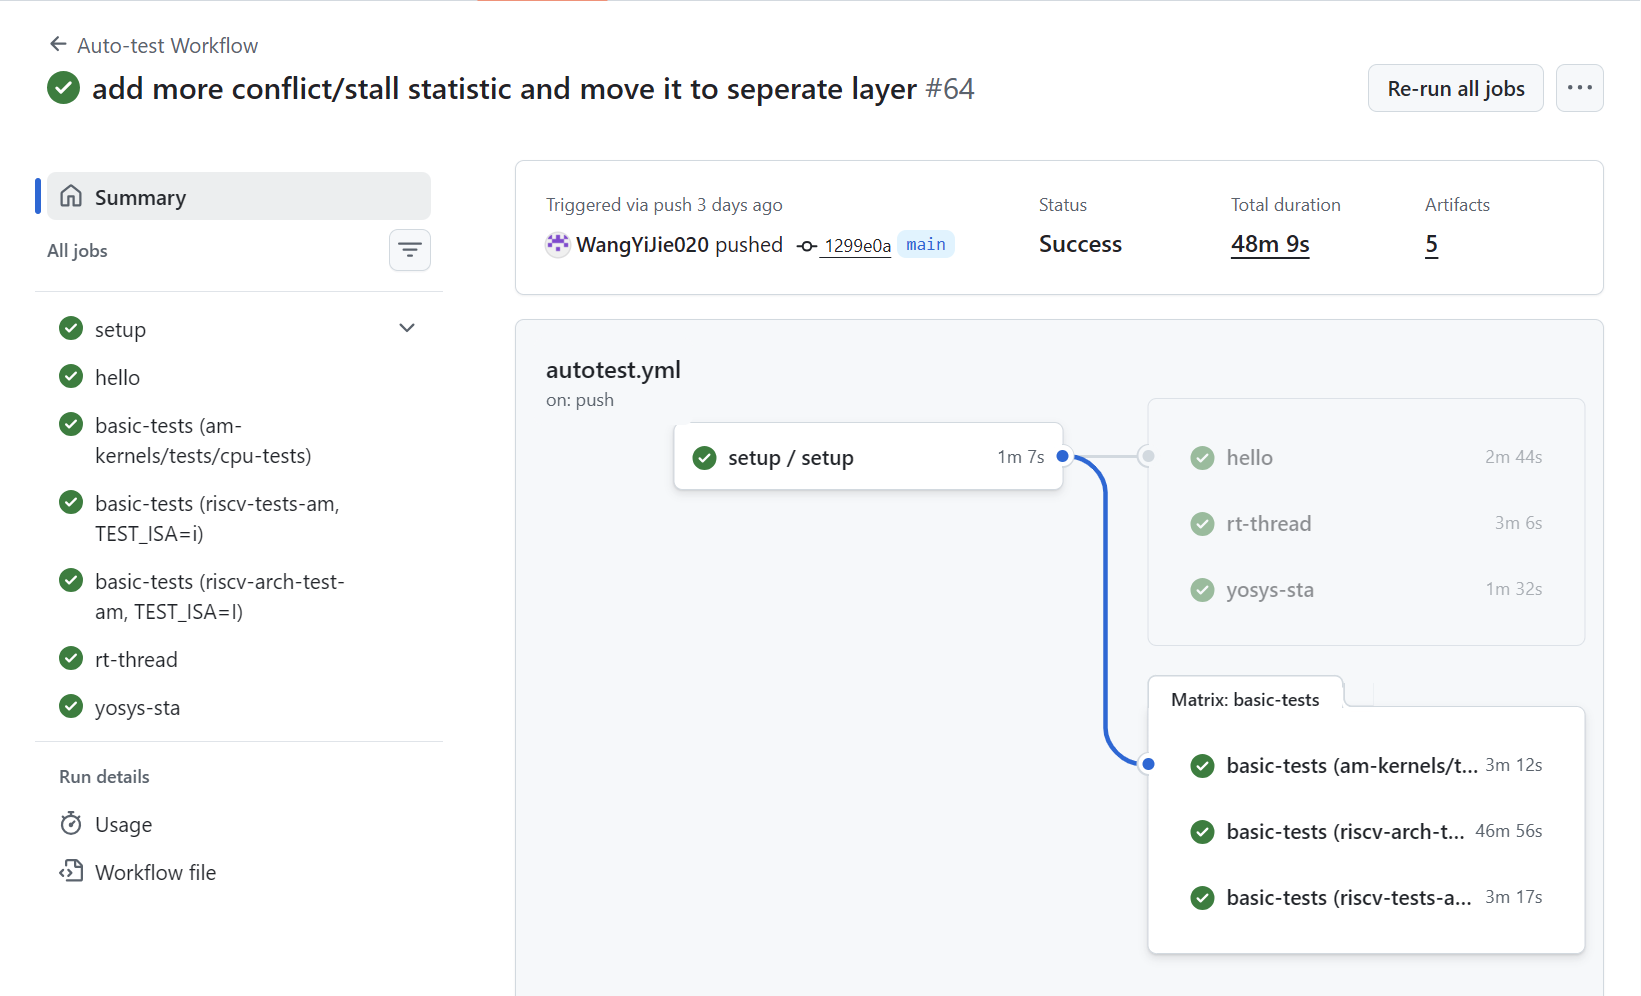
\includegraphics[width=0.92\linewidth]{verify/image10.png}
  \caption{正确性测试自动化流程界面}
\end{figure}

项目提交时的版本对应测试记录为
\href{https://github.com/HanPiM/jyd/actions/runs/29162587063}{HanPiM/jyd@585ebc2b}。

对于单元测试，项目选用了下列测试集测试每个指令以及其边界情况，从指令级别对 CPU 进行了较为完备的基础测试。

\begin{itemize}
	\item \href{https://github.com/NJU-ProjectN/riscv-tests-am}{NJU-ProjectN/riscv-tests-am}：移植到 AM \footnote{南京大学计算机实验中对裸机环境的一层抽象环境} 的 \href{https://github.com/riscv-software-src/riscv-tests}{riscv-tests} 测试集。
  \item \href{https://github.com/NJU-ProjectN/riscv-arch-test-am}{NJU-ProjectN/riscv-arch-test-am}：移植到 AM 的 \href{https://github.com/riscv/riscv-arch-test}{riscv-arch-test} 测试集。
  \item 对于小规模程序测试，使用了 \href{https://github.com/NJU-ProjectN/am-kernels}{NJU-ProjectN/am-kernels: AbstractMachine kernels}，其中 tests/cpu-tests 提供了简易程序级测试负载。
\end{itemize}

\subsubsection{RV32I CPU性能测试}

性能测试选用了官方给出的 src0、src1、src2 三个性能测试，以及额外的由 NJU-ProjectN/am-kernels 移植提供的 coremark、dhrystone 跑分测试项。因为仿真的时序信息不准确，Counter 计时器连接的时钟和 CPU 时钟相同，预测的运行时间通过 Cycle 数另外计算。

\begin{figure}[H]
  \centering
  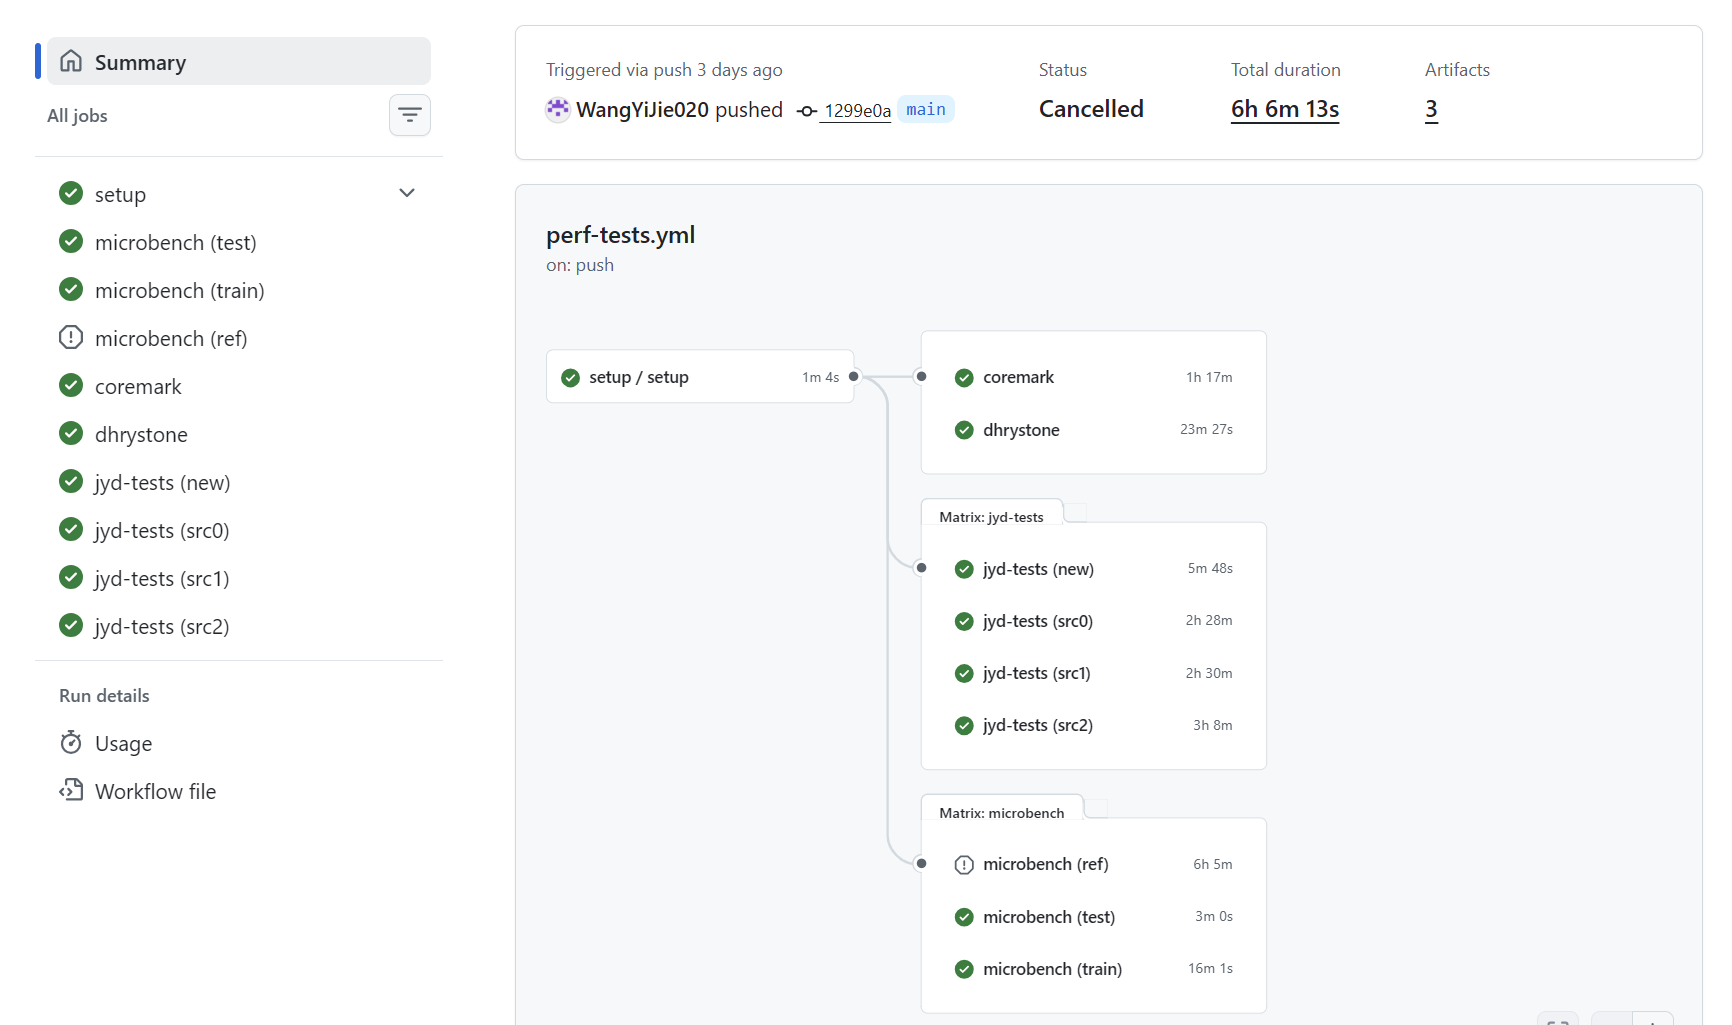
\includegraphics[width=\linewidth]{verify/image11.png}
  \caption{性能测试自动化流程界面}
\end{figure}

\subsubsection{RV32I CPU 其他测试}

CPU 支持了部分 CSR 寄存器：mcycle(h)、mstatus、mepc、mtvec、marchid、mvendorid，支持了 ecall、mret、csrrw、csrrs 指令。并基于南京大学计算机实验教学版本 RT-Thread 分支 \href{https://github.com/NJU-ProjectN/rt-thread-am}{NJU-ProjectN/rt-thread-am}（不能直接运行，仅将依赖库替换为了 AM 裸机环境），参考南京大学计算机实验的讲义\footnote{\href{https://ysyx.oscc.cc/docs/ics-pa/4.1.html\#rt-thread-\%E9\%80\%89\%E5\%81\%9A}{RT-Thread 选做讲义}。}，独立完成了软件上 BSP 部分依靠 CSR 进行上下文切换的实现，从而能够支持 RT-Thread 的运行。同时为方便测试，为 CPU 添加了仿真层面的串口可以进行输入。

% \begin{figure}[H]
%   \centering
%   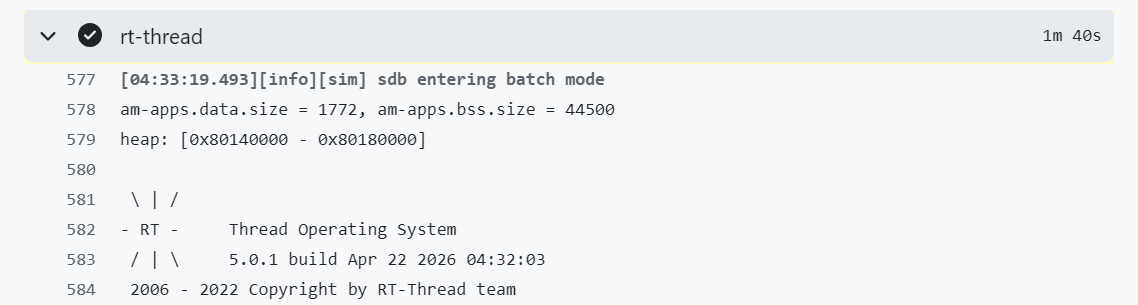
\includegraphics[width=0.82\linewidth]{verify/image12.png}
%   \caption{RT-Thread 启动输出}
% \end{figure}

自动化测试流程为使用脚本\footnote{参考了一生一芯项目 B 阶段 CI 测试的脚本。}启动仿真后向标准输入流写入测试命令，监测输出是否出现预期结果。

\clearpage
\section{验证与测评结果}

\subsection{RV32I指令集测试结果}

\subsubsection{RV32I基本指令测试结果}

\begin{figure}[H]
  \centering
  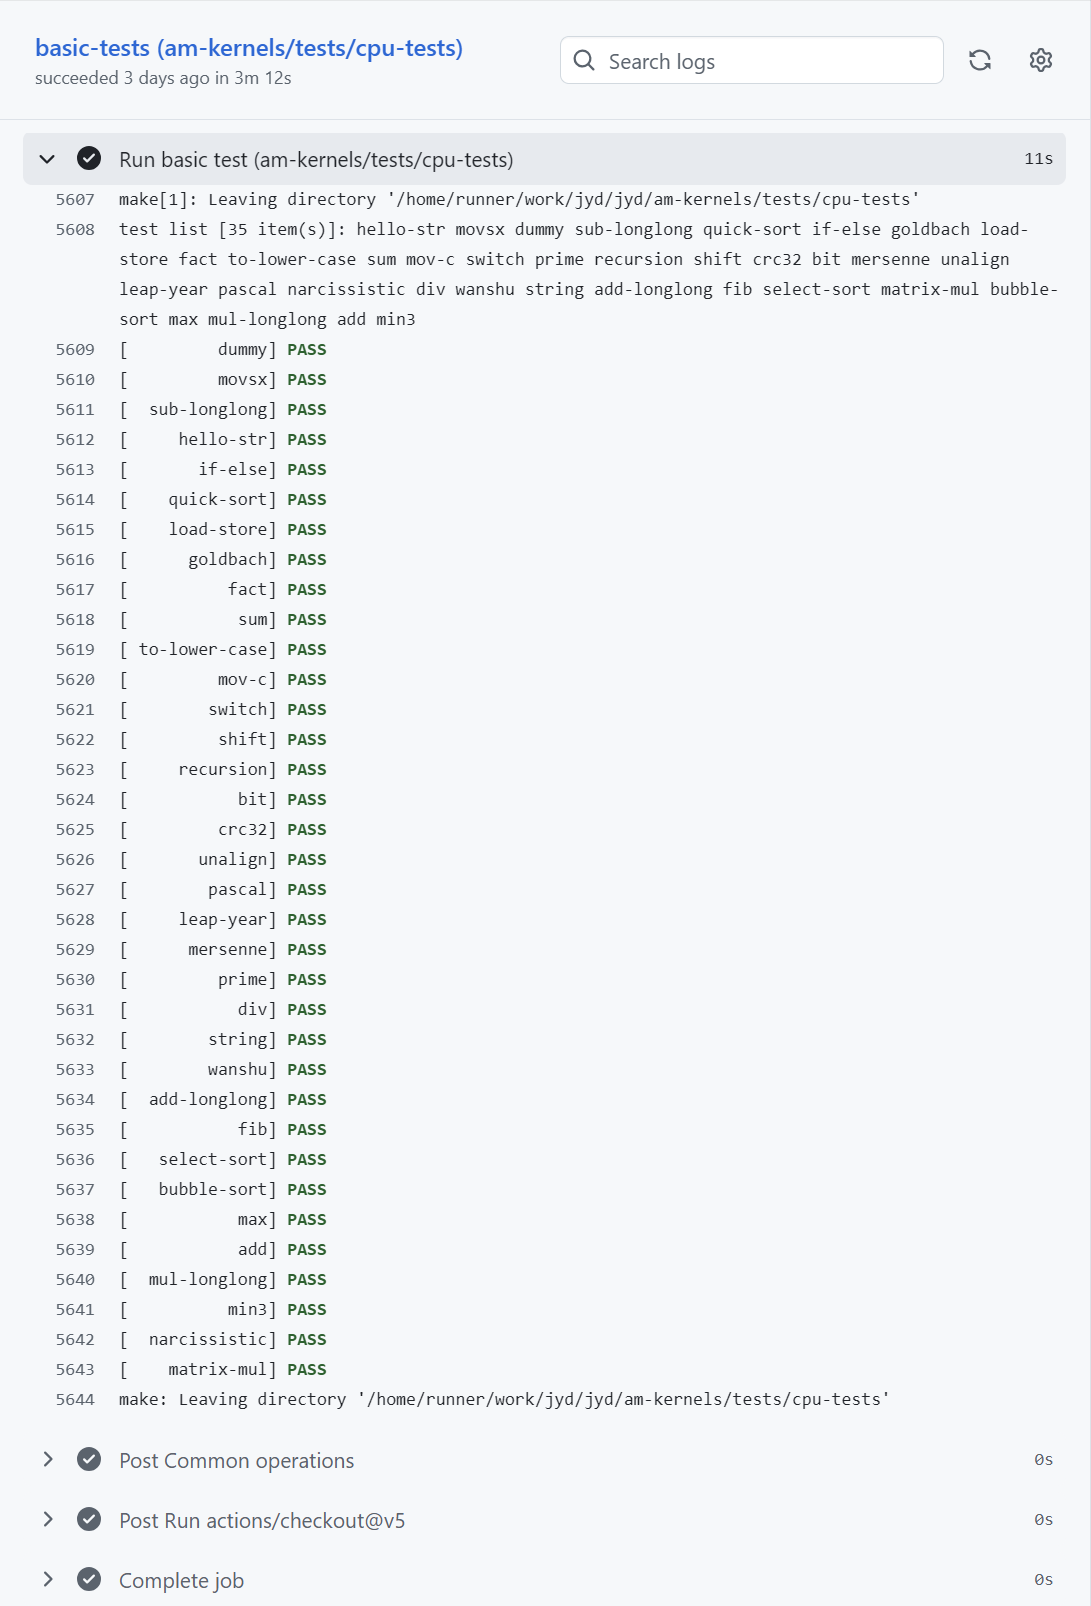
\includegraphics[height=0.64\textheight,trim=0 0 669bp 0,clip]{verify/image13.png}%
  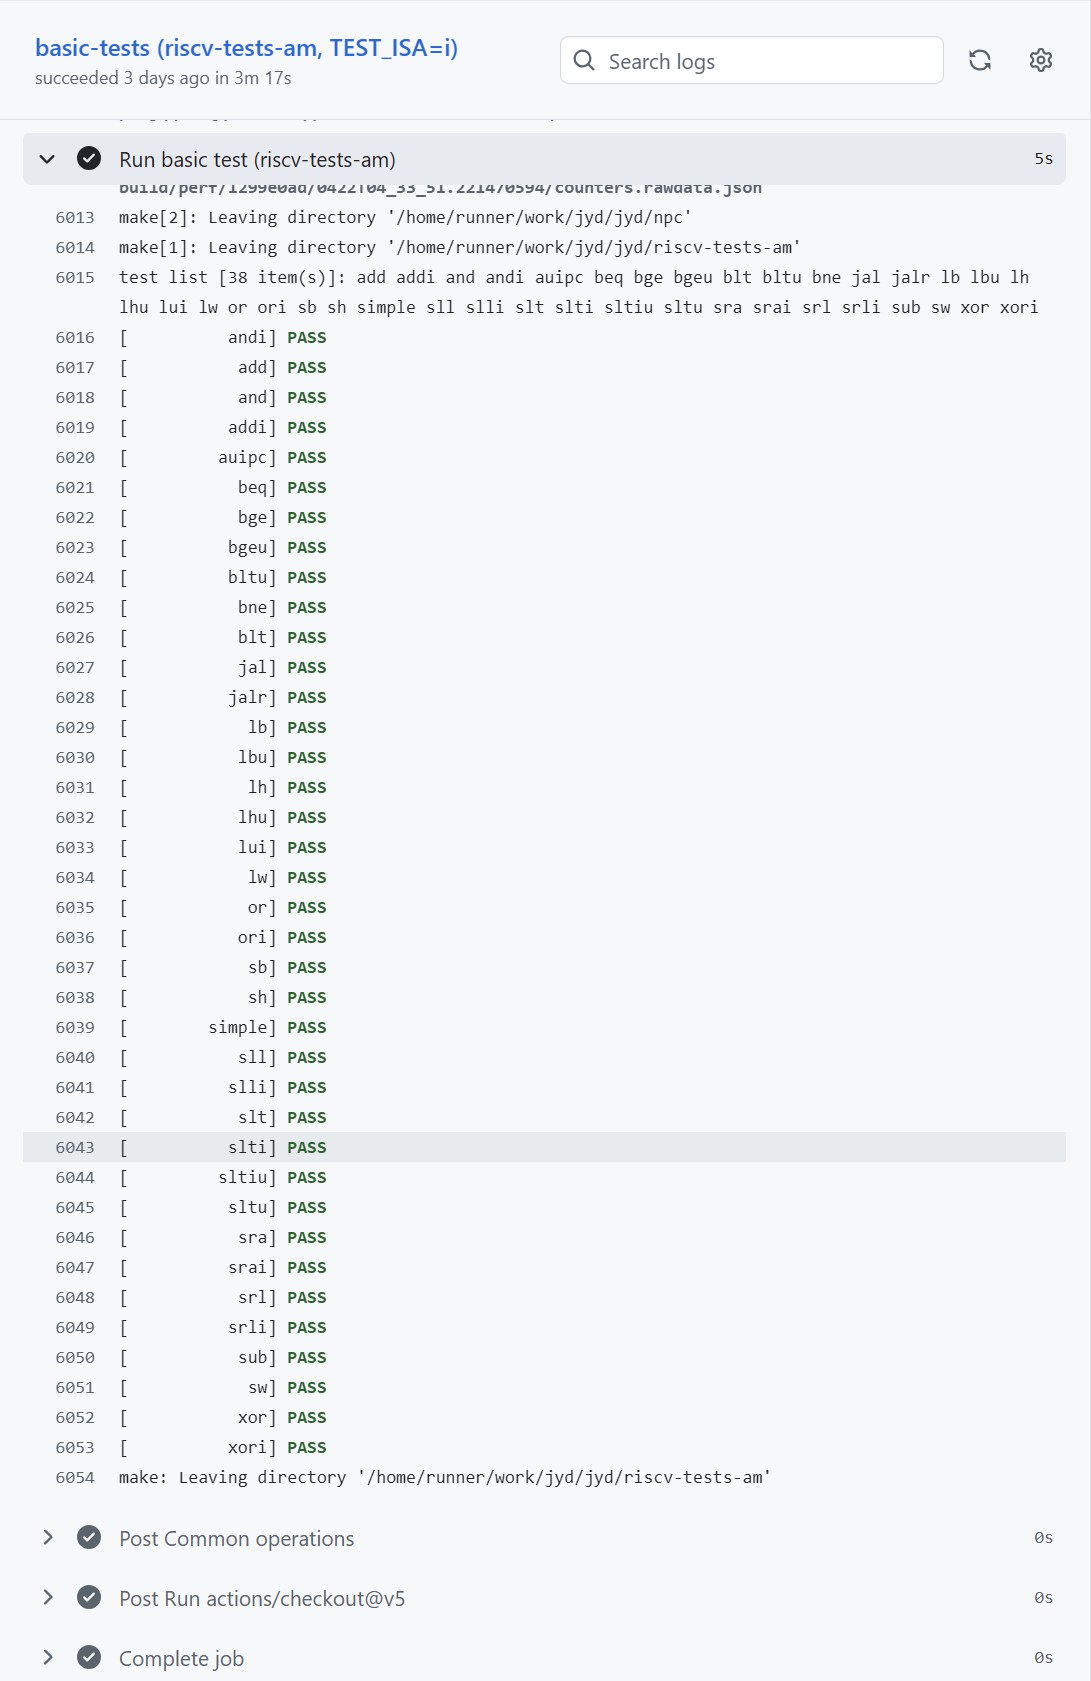
\includegraphics[height=0.64\textheight,trim=0 0 644bp 0,clip]{verify/image14.png}%
  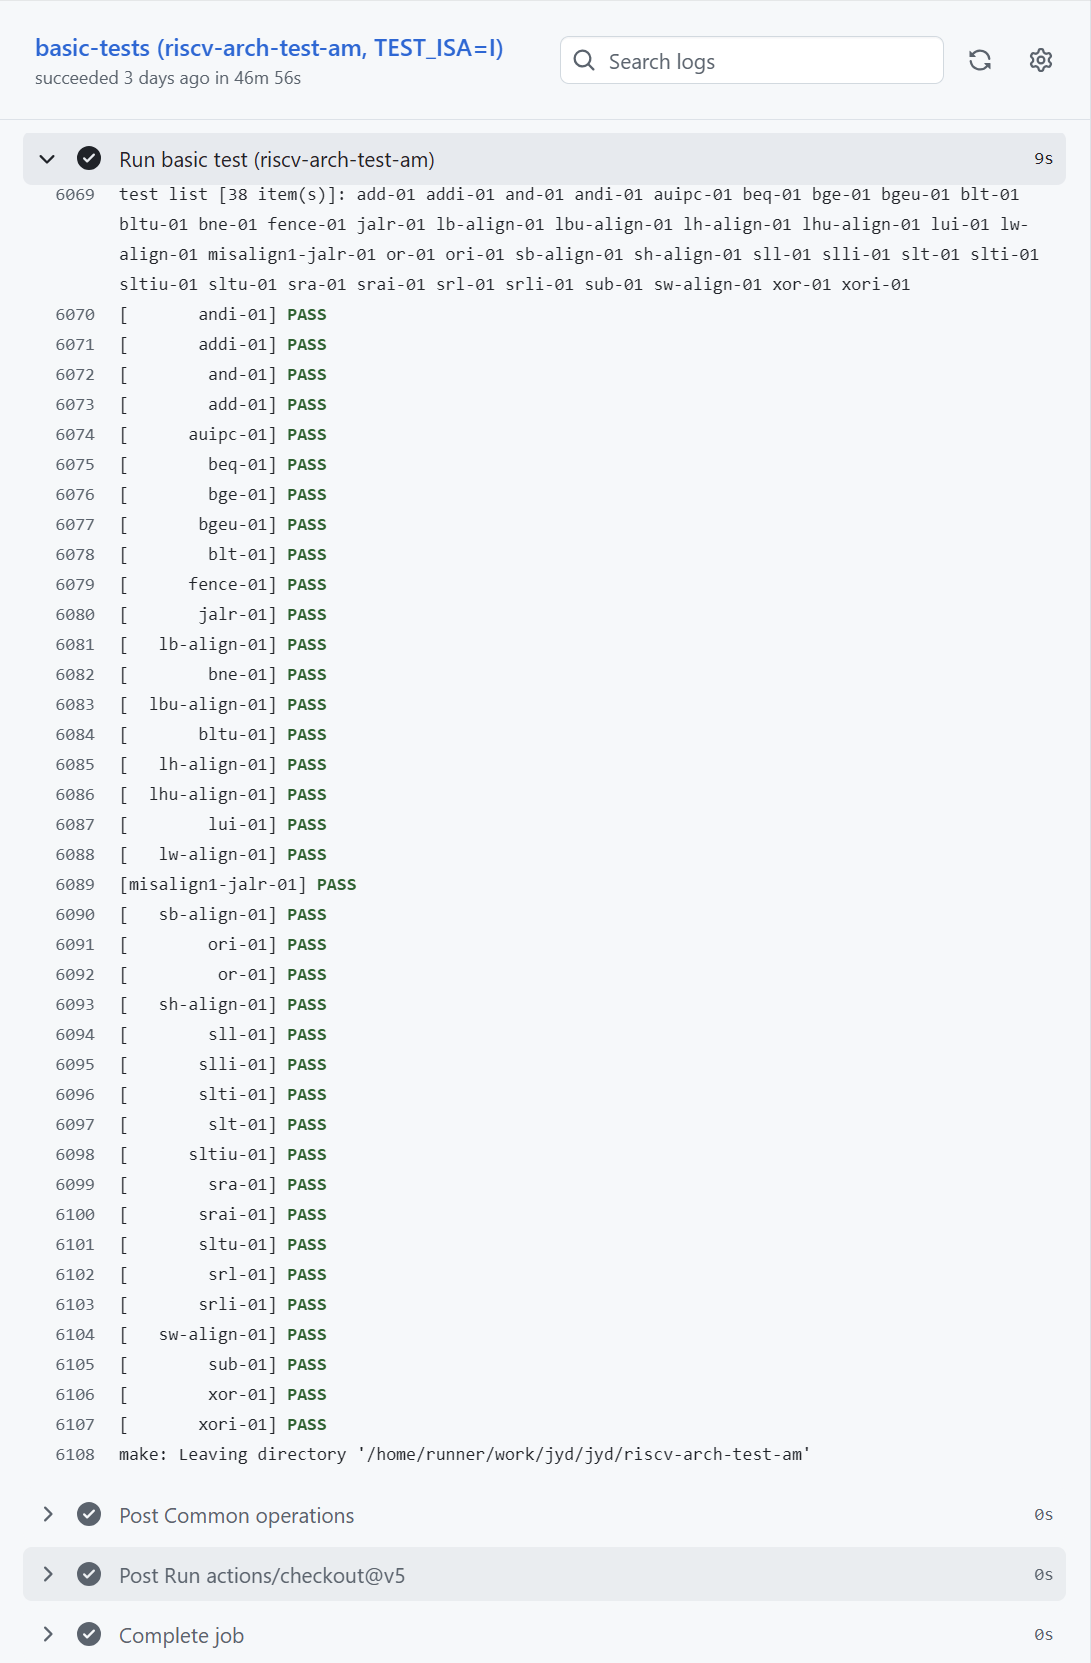
\includegraphics[height=0.64\textheight,trim=0 0 654bp 0,clip]{verify/image15.png}
  \caption{RV32I 基本指令测试结果截图}
\end{figure}

从图片可以看出所有测试均成功通过，表明 CPU 支持 RV32I 且能够正确处理边界样例。

\subsection{RV32I CPU性能测试结果}

\subsubsection{src0性能测试用例}

\begin{figure}[H]
  \centering
  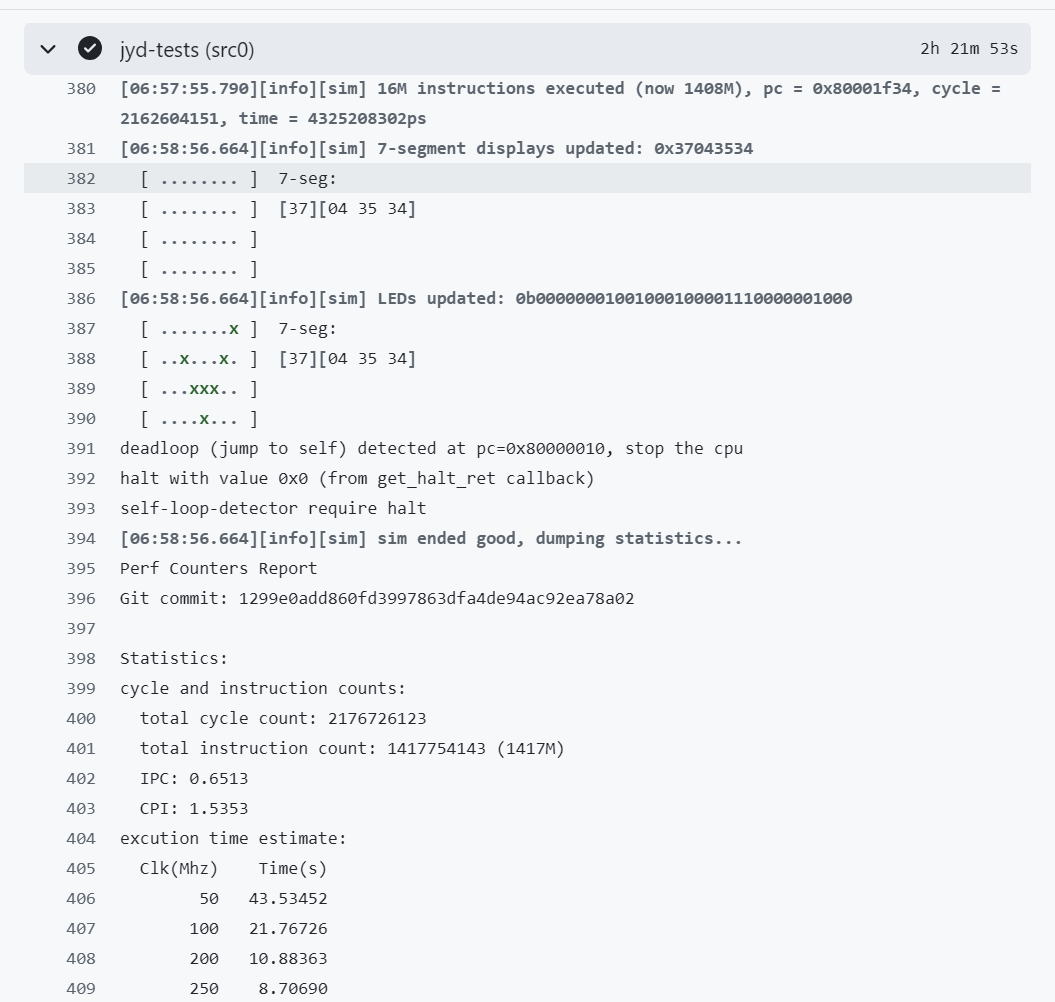
\includegraphics[width=0.84\linewidth,trim=0 365bp 0 0,clip]{verify/image16.png}
  \caption{src0 仿真日志与性能统计结果}
\end{figure}

测试程序 src0 成功在仿真末尾观测到数码管和 LED 更新为预期结果，表明 37 条指令测试和性能测试均通过。
程序最终进入 halt 死循环并被仿真正确识别。本次 CI 统计总周期数为 1,988,372,516，按 280 MHz
计算，预测运行时间为 $1,988,372,516/(280\times10^6)=7.10133$ s，与上板显示的 7.101 s 一致。

仿真性能计数器显示\footnote{性能统计截图暂沿用初赛版并裁去下方旧 CPI 数据；决赛版原始数据以本次 CI 日志为准。}
总周期数为 1988M，总动态指令数为 1417M，IPC 为 0.7130，CPI 为 1.4025。

\begin{figure}[H]
  \centering
  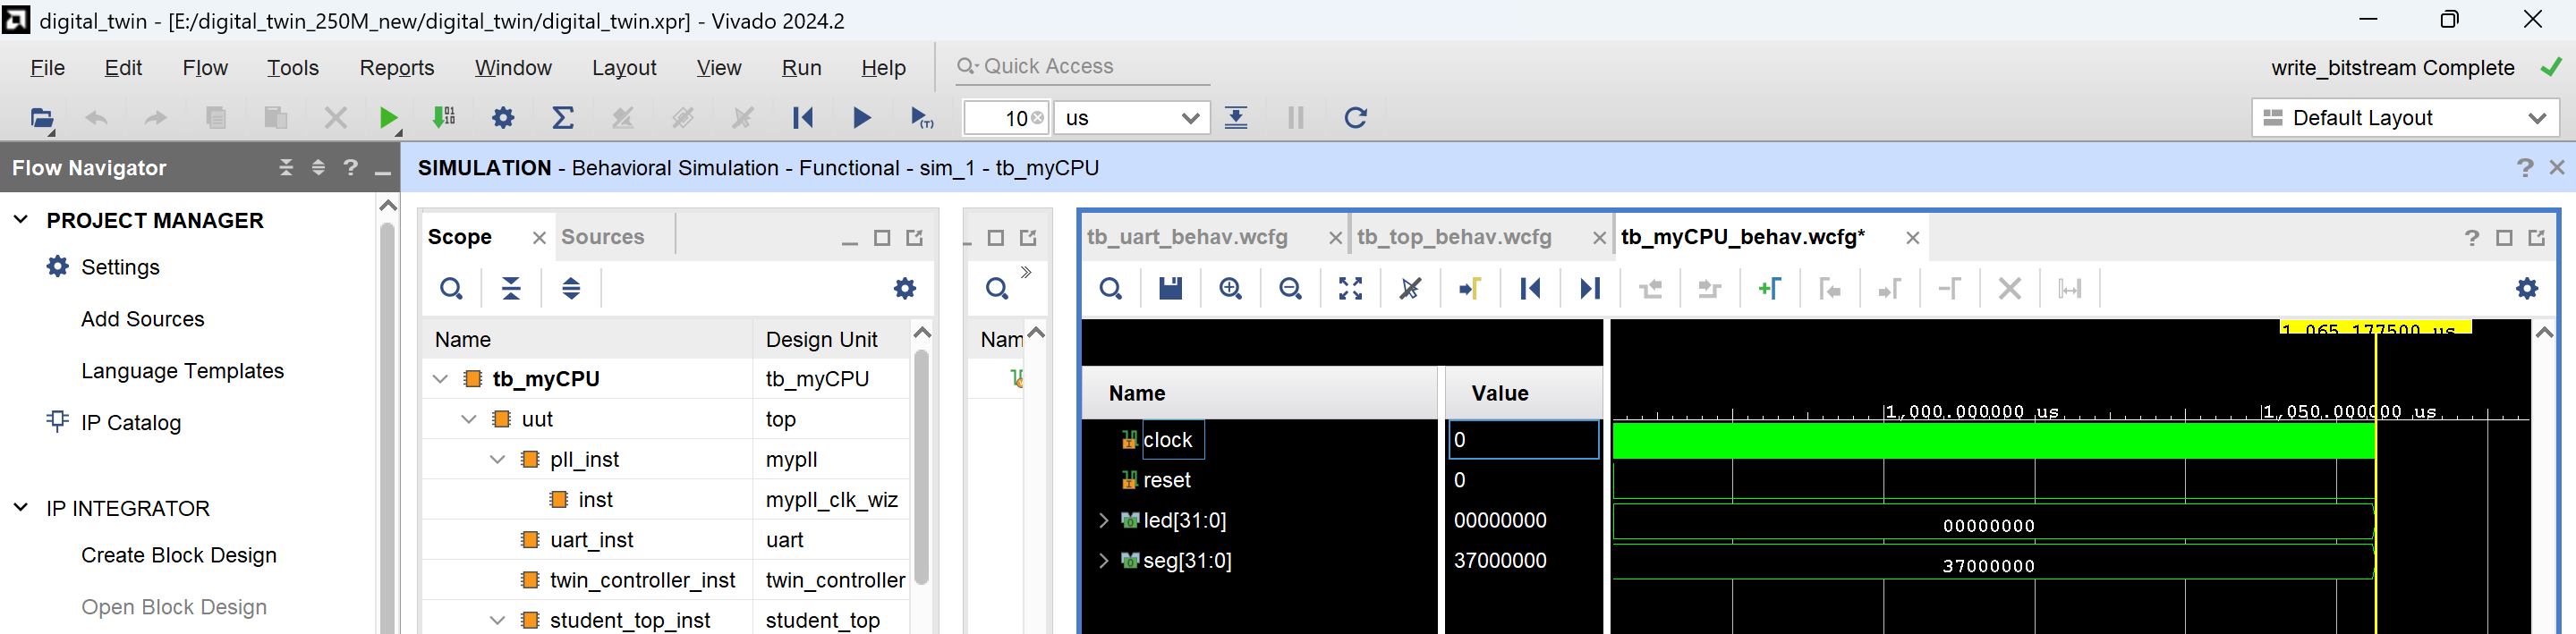
\includegraphics[width=\linewidth]{verify/image17.png}
  \caption{src0 仿真波形结果}
\end{figure}

因 Vivado 仿真速度较慢，只仿真到数码管显示 37000000 证明 37 条指令测试正确通过，未完整运行至性能测试结束。

\subsubsection{src1性能测试用例}

\begin{figure}[H]
  \centering
  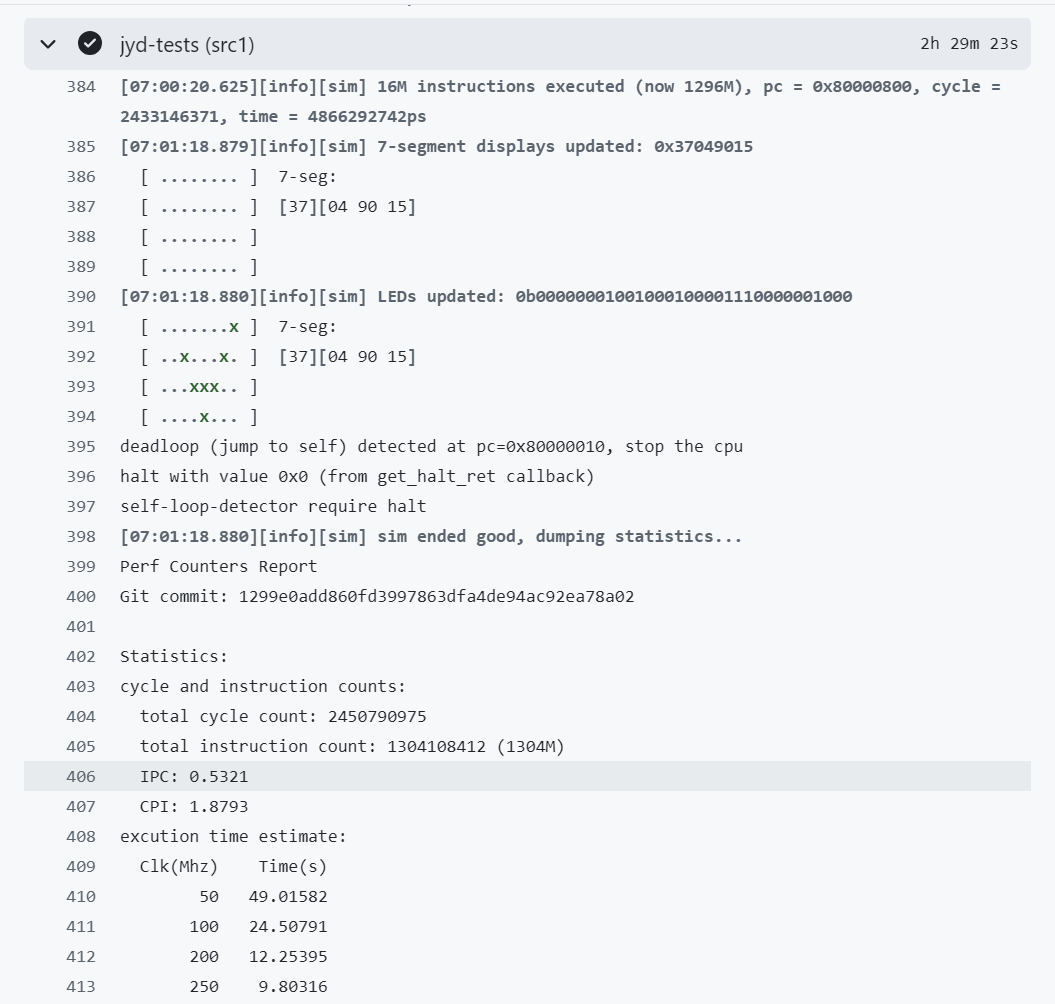
\includegraphics[width=0.82\linewidth,trim=0 350bp 0 0,clip]{verify/image18.png}
  \caption{src1 仿真日志与性能统计结果}
\end{figure}

37 条指令测试通过。总周期数为 1,973,306,668，280 MHz 预测运行时间为 7.04752 s，
与实际上板测试结果 7.047 s 一致。

仿真性能计数器显示总周期数为 1973M，总动态指令数为 1304M，IPC 为 0.6609，CPI 为 1.5131。

\begin{figure}[H]
  \centering
  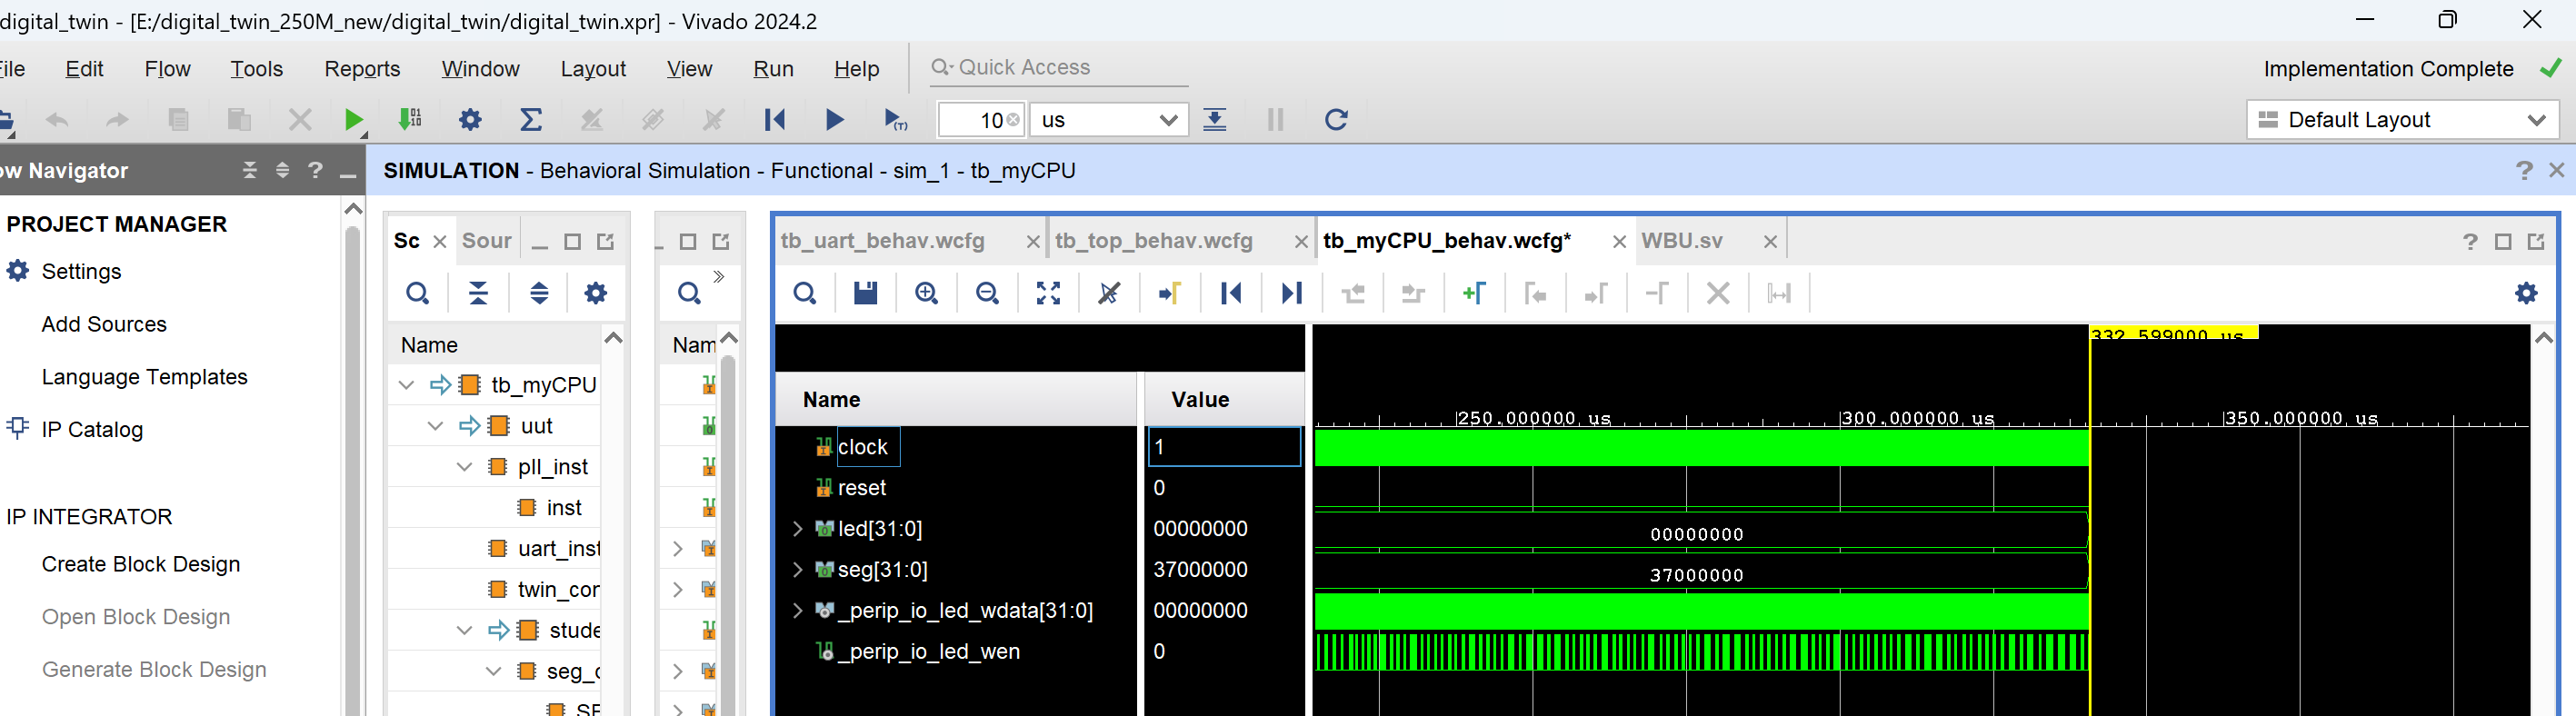
\includegraphics[width=\linewidth]{verify/image19.png}
  \caption{src1 仿真波形结果}
\end{figure}

由图可知，数码管显示 37000000 证明 37 条指令测试正确通过。

\subsubsection{src2性能测试用例}

\begin{figure}[H]
  \centering
  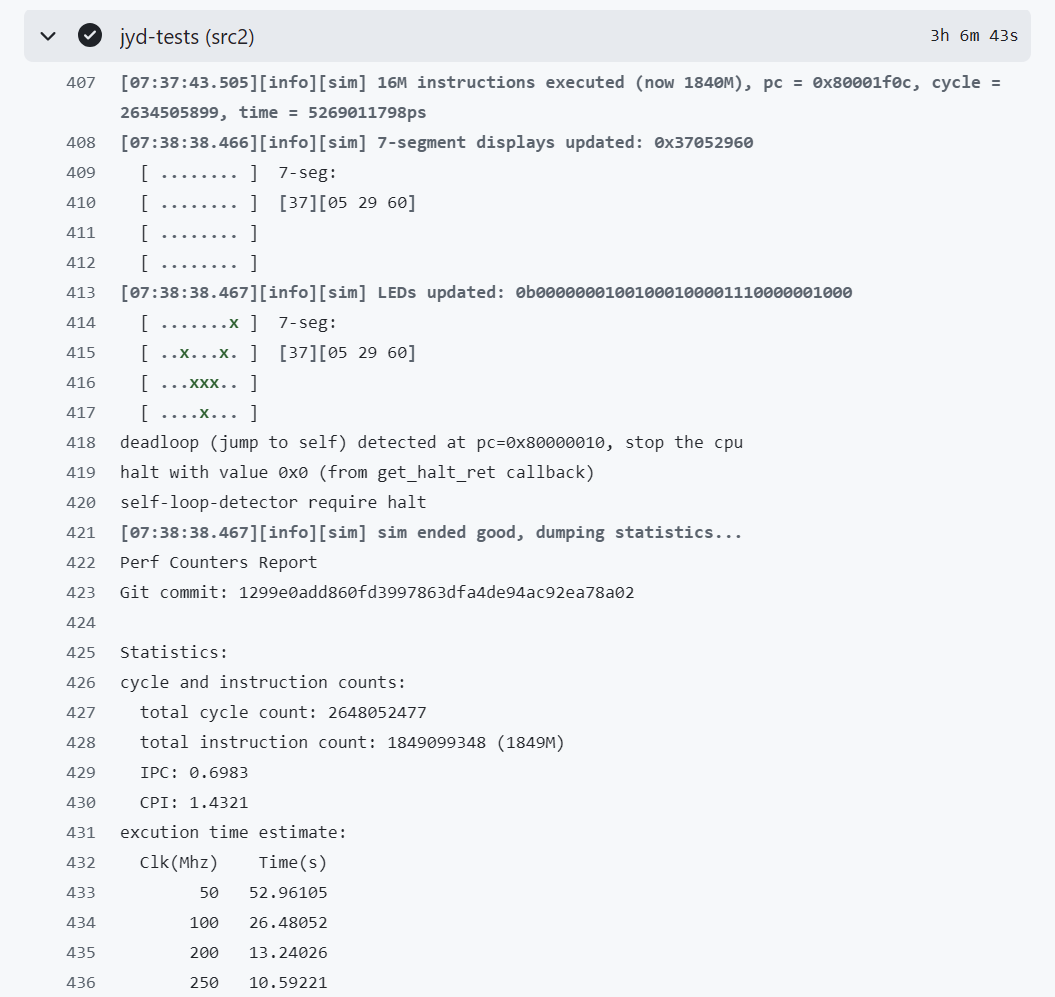
\includegraphics[width=0.84\linewidth,trim=0 340bp 0 0,clip]{verify/image20.png}
  \caption{src2 仿真日志与性能统计结果}
\end{figure}

37 条指令测试通过。总周期数为 2,585,374,792，280 MHz 预测运行时间为 9.23348 s，
与实际上板测试结果 9.233 s 一致。

仿真性能计数器显示总周期数为 2585M，总动态指令数为 1849M，IPC 为 0.7152，CPI 为 1.3982。

\begin{figure}[H]
  \centering
  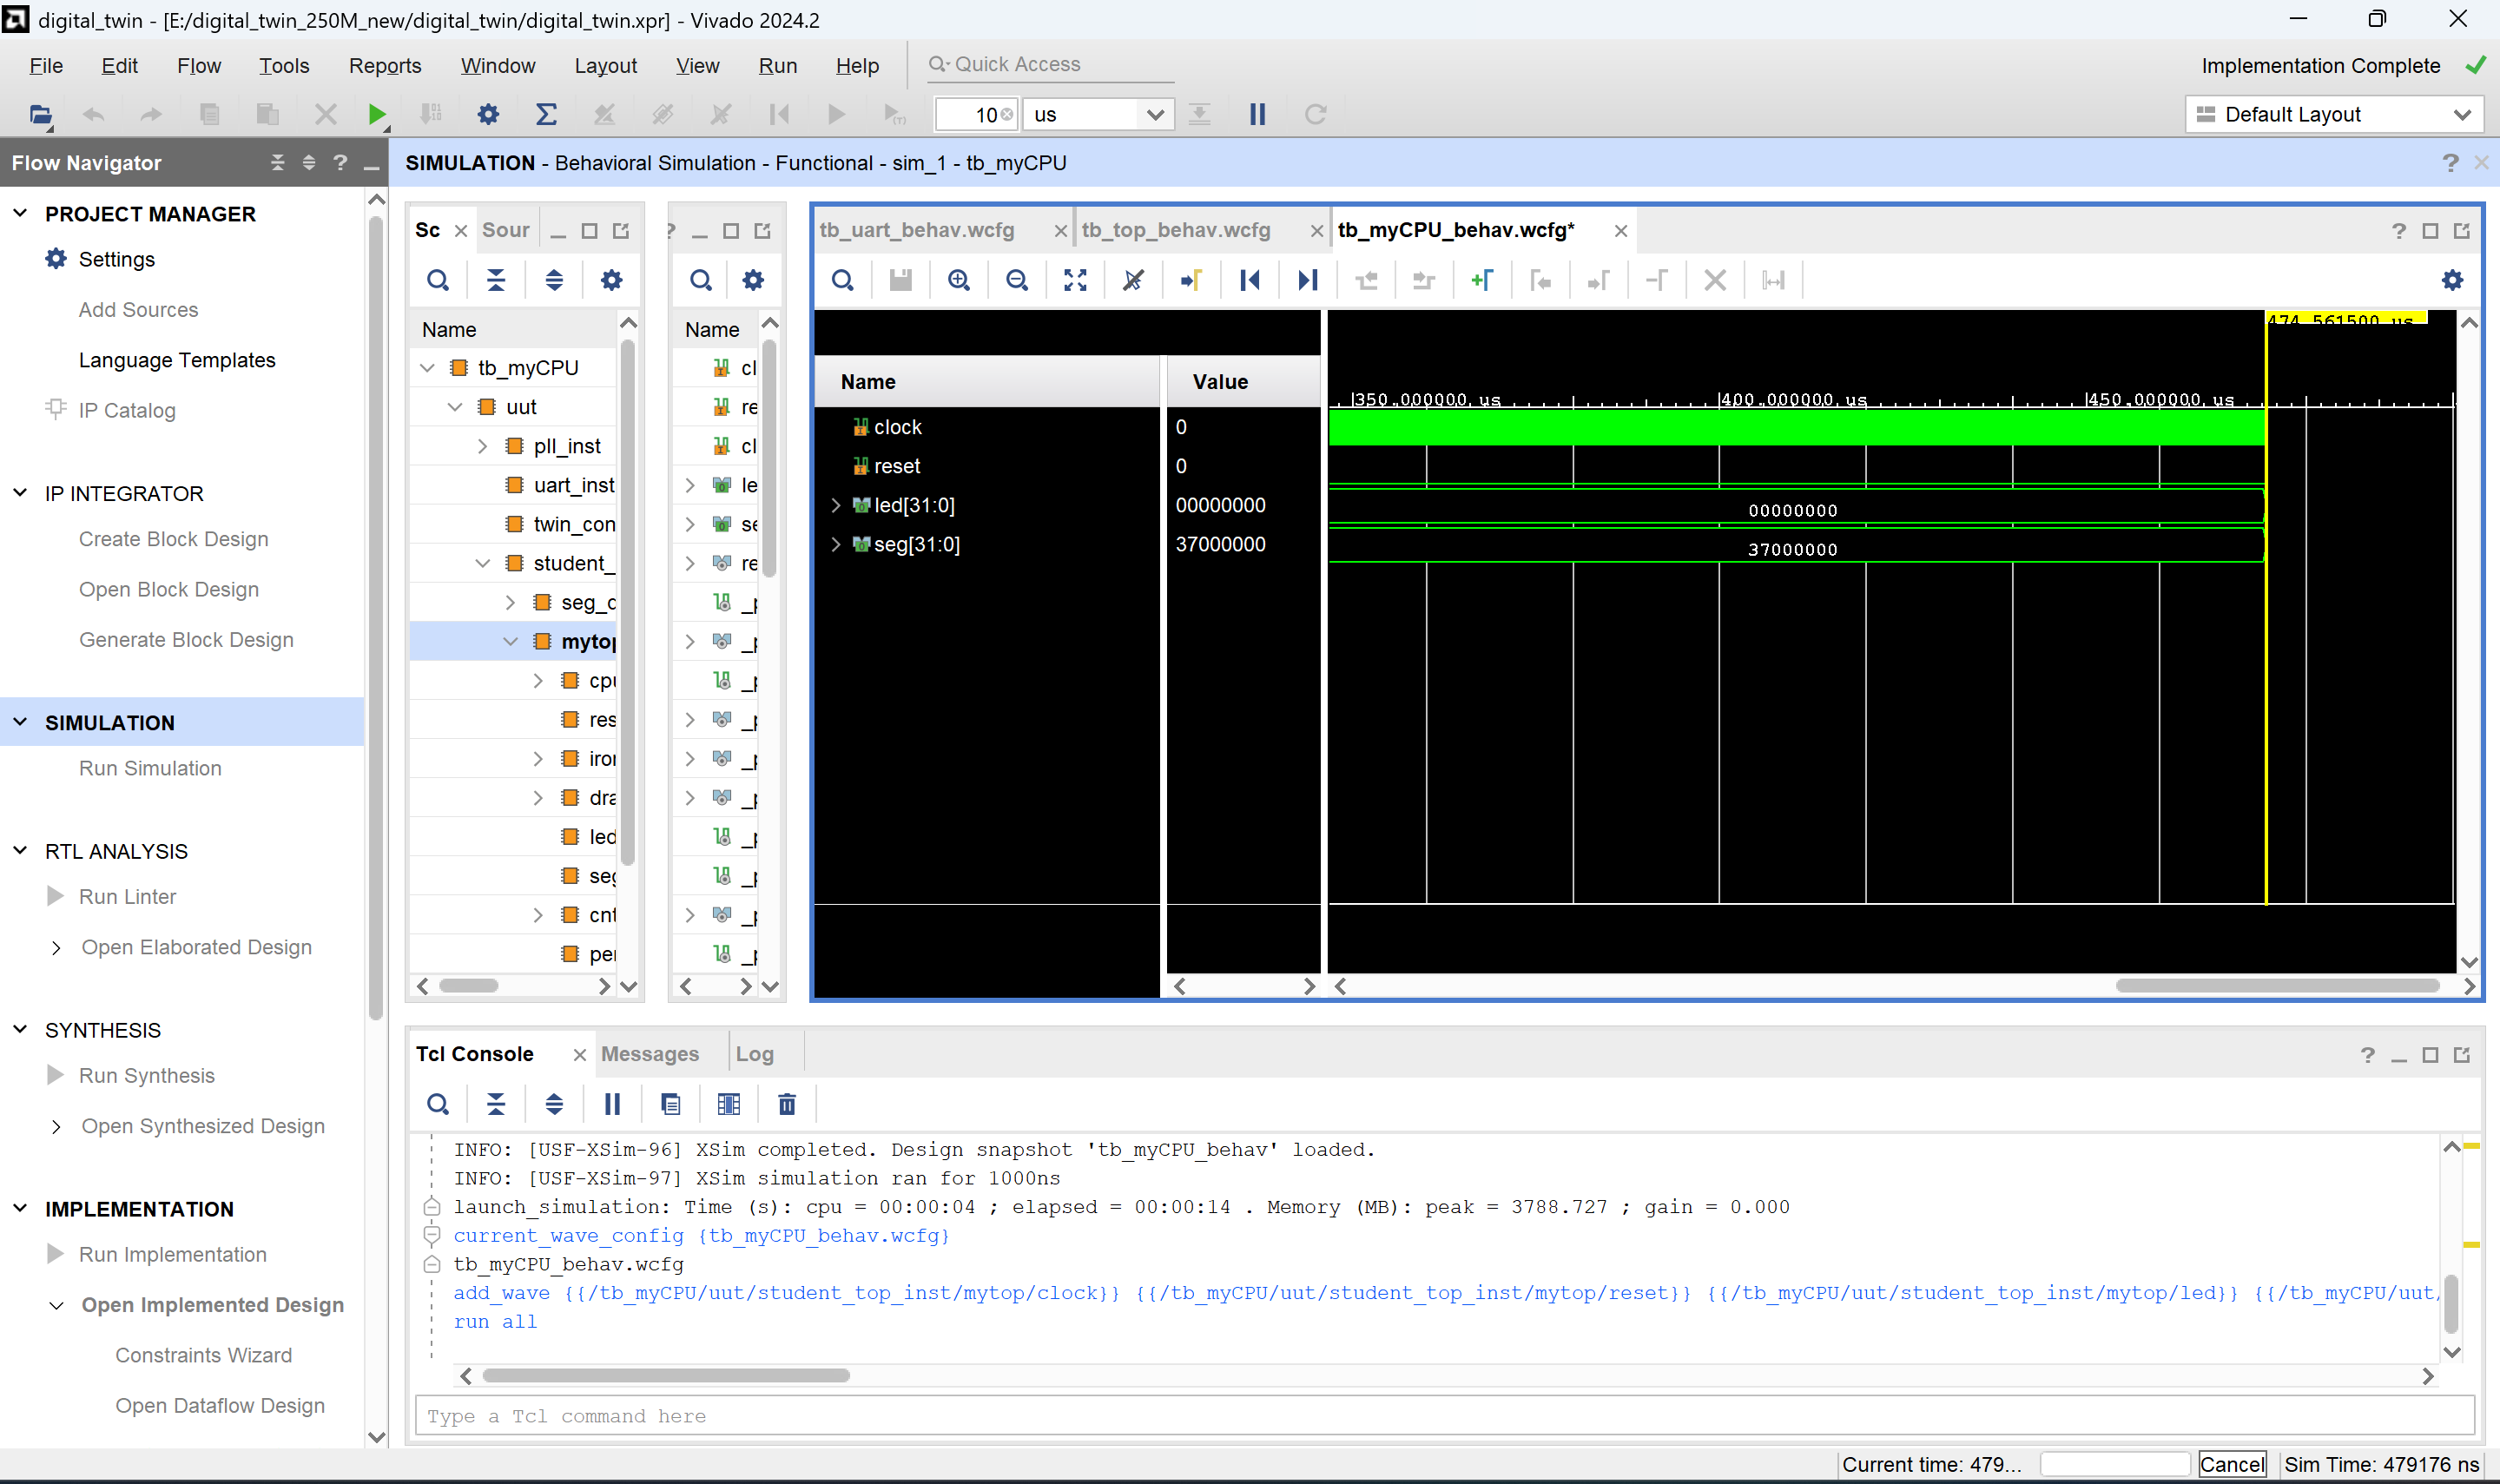
\includegraphics[width=\linewidth]{verify/image21.png}
  \caption{src2 仿真波形结果}
\end{figure}

由图可知，数码管显示 37000000 证明 37 条指令测试正确通过。

\begin{threelongtable}{@{}
  C{0.12\linewidth}
  C{0.16\linewidth}
  C{0.16\linewidth}
  C{0.10\linewidth}
  C{0.10\linewidth}
  C{0.15\linewidth}@{}}
\caption{src0、src1、src2性能统计结果汇总}\\
\toprule
测试用例 & 总周期数 & 总指令数 & IPC & CPI & 280 MHz时间/s \\
\midrule
\endfirsthead
\toprule
测试用例 & 总周期数 & 总指令数 & IPC & CPI & 280 MHz时间/s \\
\midrule
\endhead
\bottomrule
\endlastfoot
src0 & 1988M & 1417M & 0.7130 & 1.4025 & 7.10133 \\
src1 & 1973M & 1304M & 0.6609 & 1.5131 & 7.04752 \\
src2 & 2585M & 1849M & 0.7152 & 1.3982 & 9.23348 \\
\end{threelongtable}

三组程序按周期数计算得到的 280 MHz 估算时间均与上板数码管显示结果一致。src2 的 IPC 最高、
CPI 最低；src1 的 CPI 相对较高，但相比初赛版本已有明显改善。

\subsubsection{coremark 性能测试用例}

\begin{figure}[H]
  \centering
  % 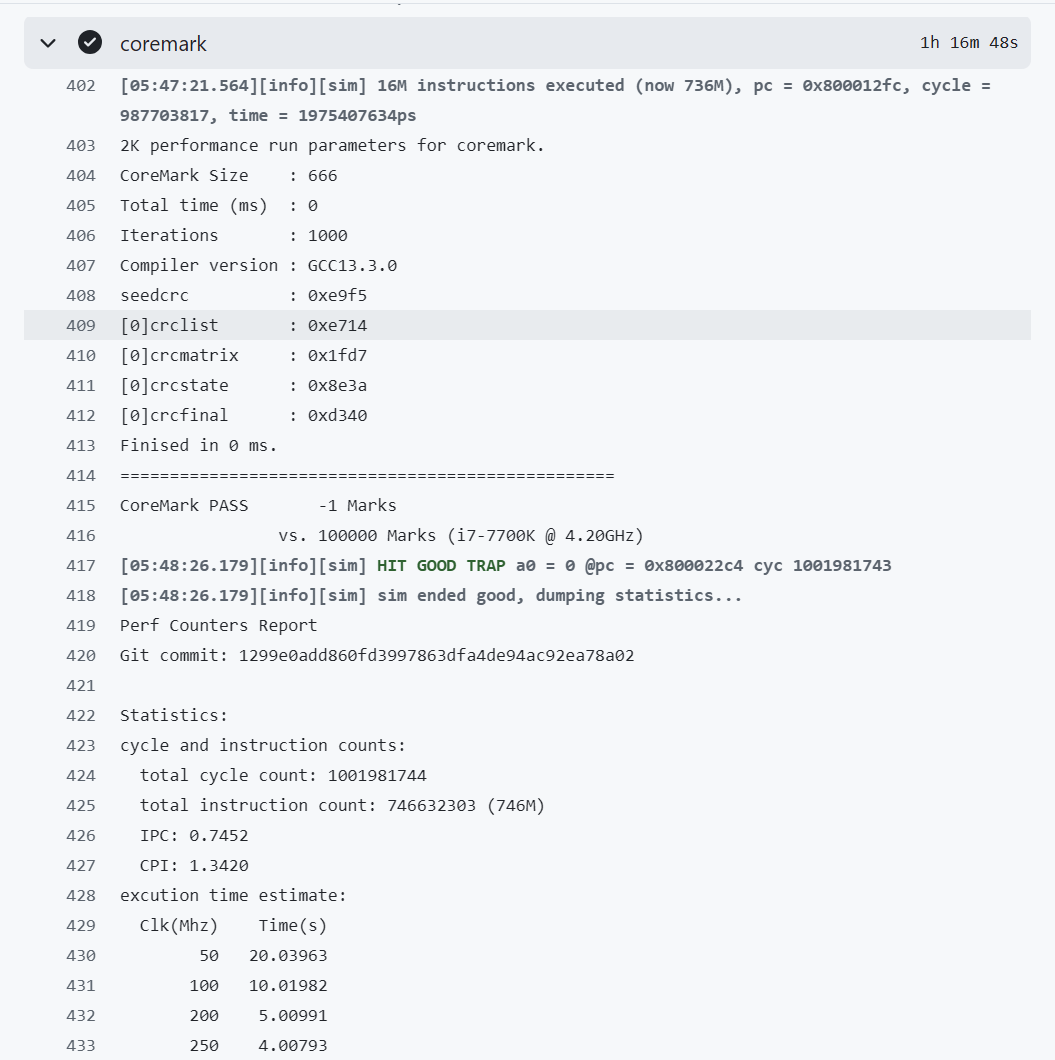
\includegraphics[width=0.45\linewidth]{verify/image22.png}\hfill
  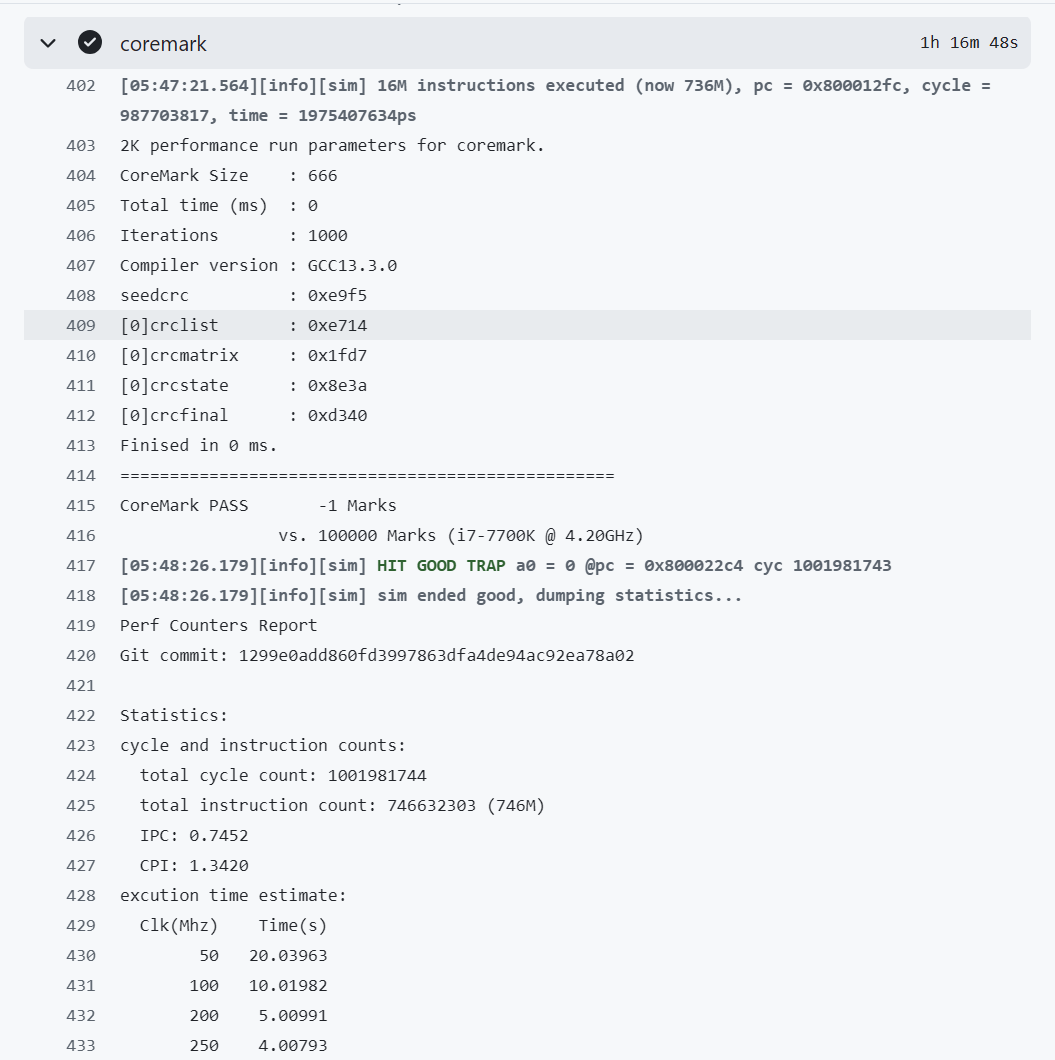
\includegraphics[width=0.82\linewidth,trim=0 440bp 0 0,clip]{verify/image22.png}
  \caption{coremark 测试结果截图}
\end{figure}

本次 CI 完成 1000 次迭代，共执行 472,993,621 周期，IPC 为 0.6625、CPI 为 1.5094。
按 280 MHz 计算运行时间为 1.68926 s，CI 输出的 CoreMark 结果为 308：

\[
  \text{CoreMark} = 308
\]

或者归一化：

\[
  \text{CoreMark/MHz} = \frac{308}{280} = 1.10
\]

达到基础顺序执行处理器的预期水平。

\subsubsection{dhrystone 性能测试用例}

\begin{figure}[H]
  \centering
  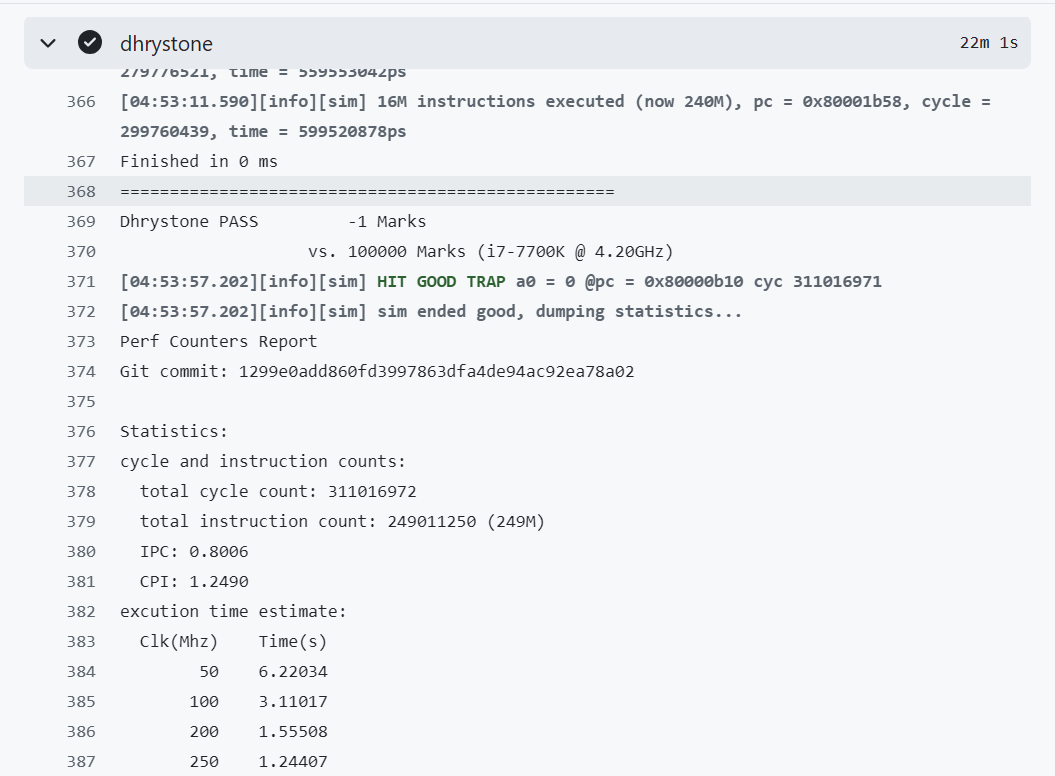
\includegraphics[width=0.82\linewidth,trim=0 545bp 0 0,clip]{verify/image23.png}
  \caption{dhrystone 测试结果截图}
\end{figure}

CPI 为 1.2873（IPC 为 0.7768），总周期数为 302,517,149；按 280 MHz 计算，
500000 次迭代的估算时间为 1.08042 s：

\[
  \text{Dhrystones/s} = \frac{\text{NUMBER\_OF\_RUNS}}{\text{Time}}
\]

\[
  \frac{500000}{1.080418389} \approx 462783.69\text{~Dhrystones/s}
\]

DMIPS 公式：

\[
  \text{DMIPS} = \frac{\text{Dhrystones/s}}{1757} \approx 263.39
\]

归一化：

\[
  \text{DMIPS/MHz} = \frac{263.39}{280} \approx 0.941
\]

达到基础顺序执行处理器的预期水平。

\subsection{RV32I CPU其他测试结果}

下面的图片展示了在 RT-Thread 上运行 version、free 等基础指令以及嵌入的 hello 和 microbench 程序。

\begin{figure}[H]
  \centering
  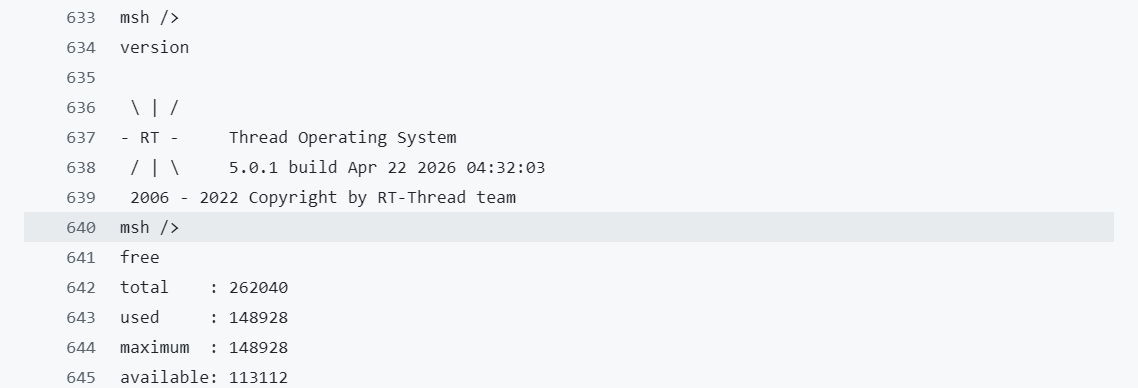
\includegraphics[width=\linewidth]{verify/image24.png}
  \vspace{0.3em}
  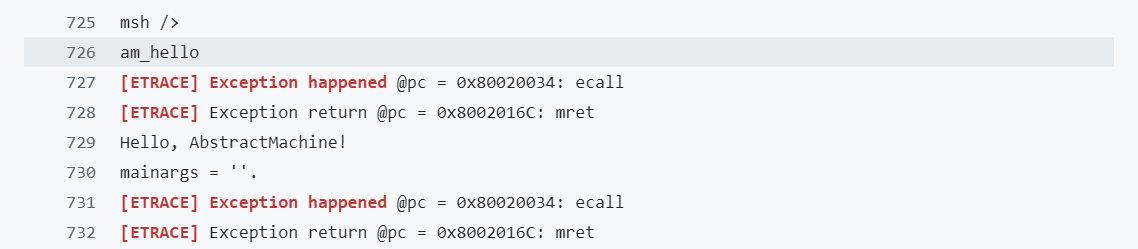
\includegraphics[width=\linewidth]{verify/image25.png}
  \vspace{0.3em}
  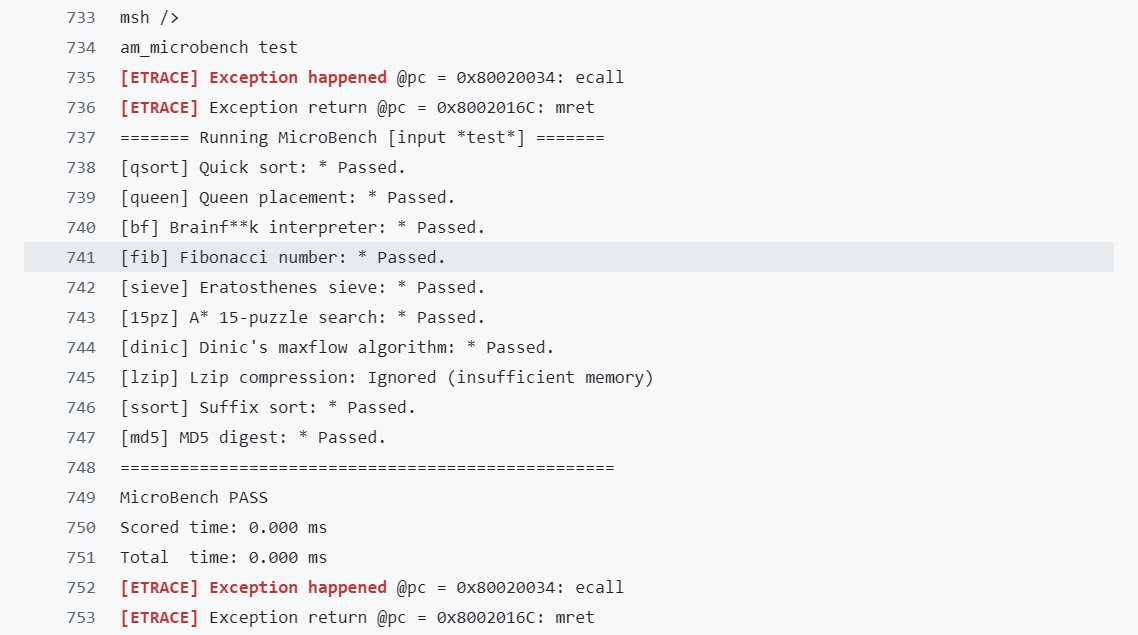
\includegraphics[width=\linewidth]{verify/image26.png}
  \vspace{0.3em}
  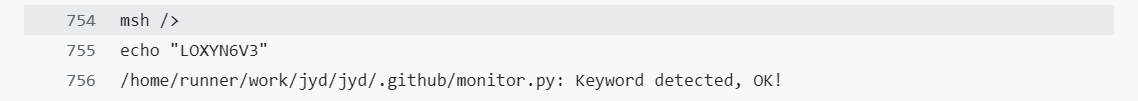
\includegraphics[width=\linewidth]{verify/image27.png}
  \caption{RT-Thread 自动化测试输出节选}
\end{figure}

最后的 echo 测试输出了预期的随机字符串，从而使 monitor 认为行为正确直接结束了测试，没有将其输出回放到 CI 的标准输出。综上表明仿真环境运行正常，CI 测试通过。

\begin{figure}[H]
  \centering
  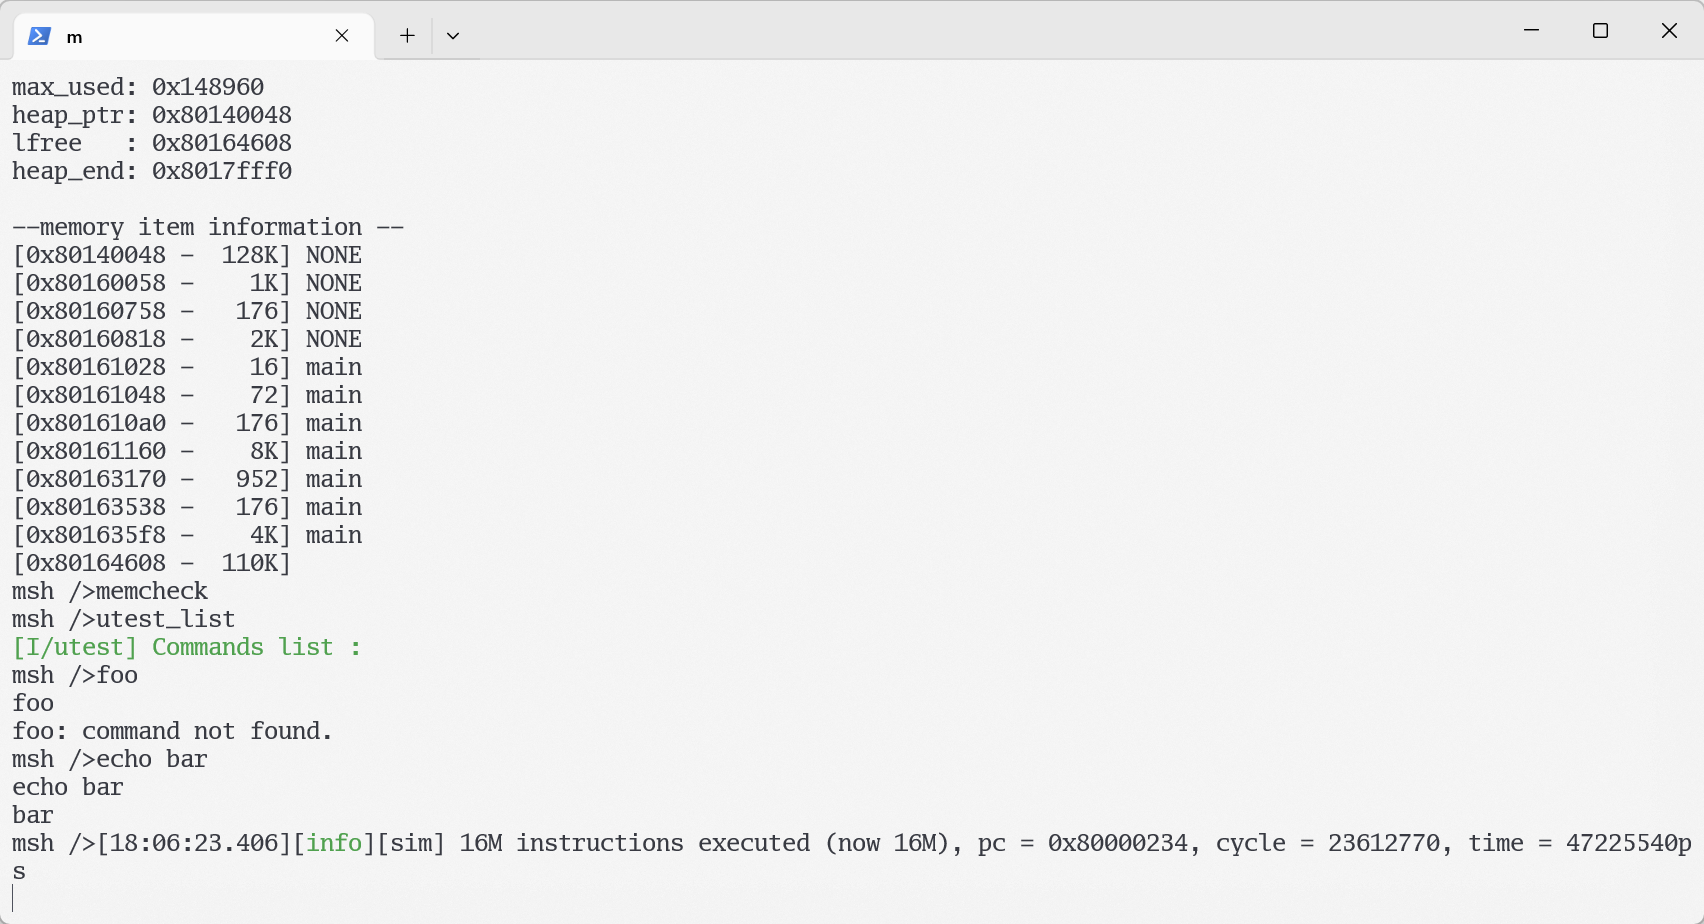
\includegraphics[width=0.9\linewidth]{verify/image28.png}
  \caption{RT-Thread 本地交互测试}
\end{figure}

本地环境通过仿真串口输入进行测试，行为符合预期，测试通过。

\newpage

\subsection{数字孪生运行截图/照片}

下列截图为分赛区决赛工程在竞业达数字孪生平台上的实际运行结果。

\begin{figure}[H]
  \centering
  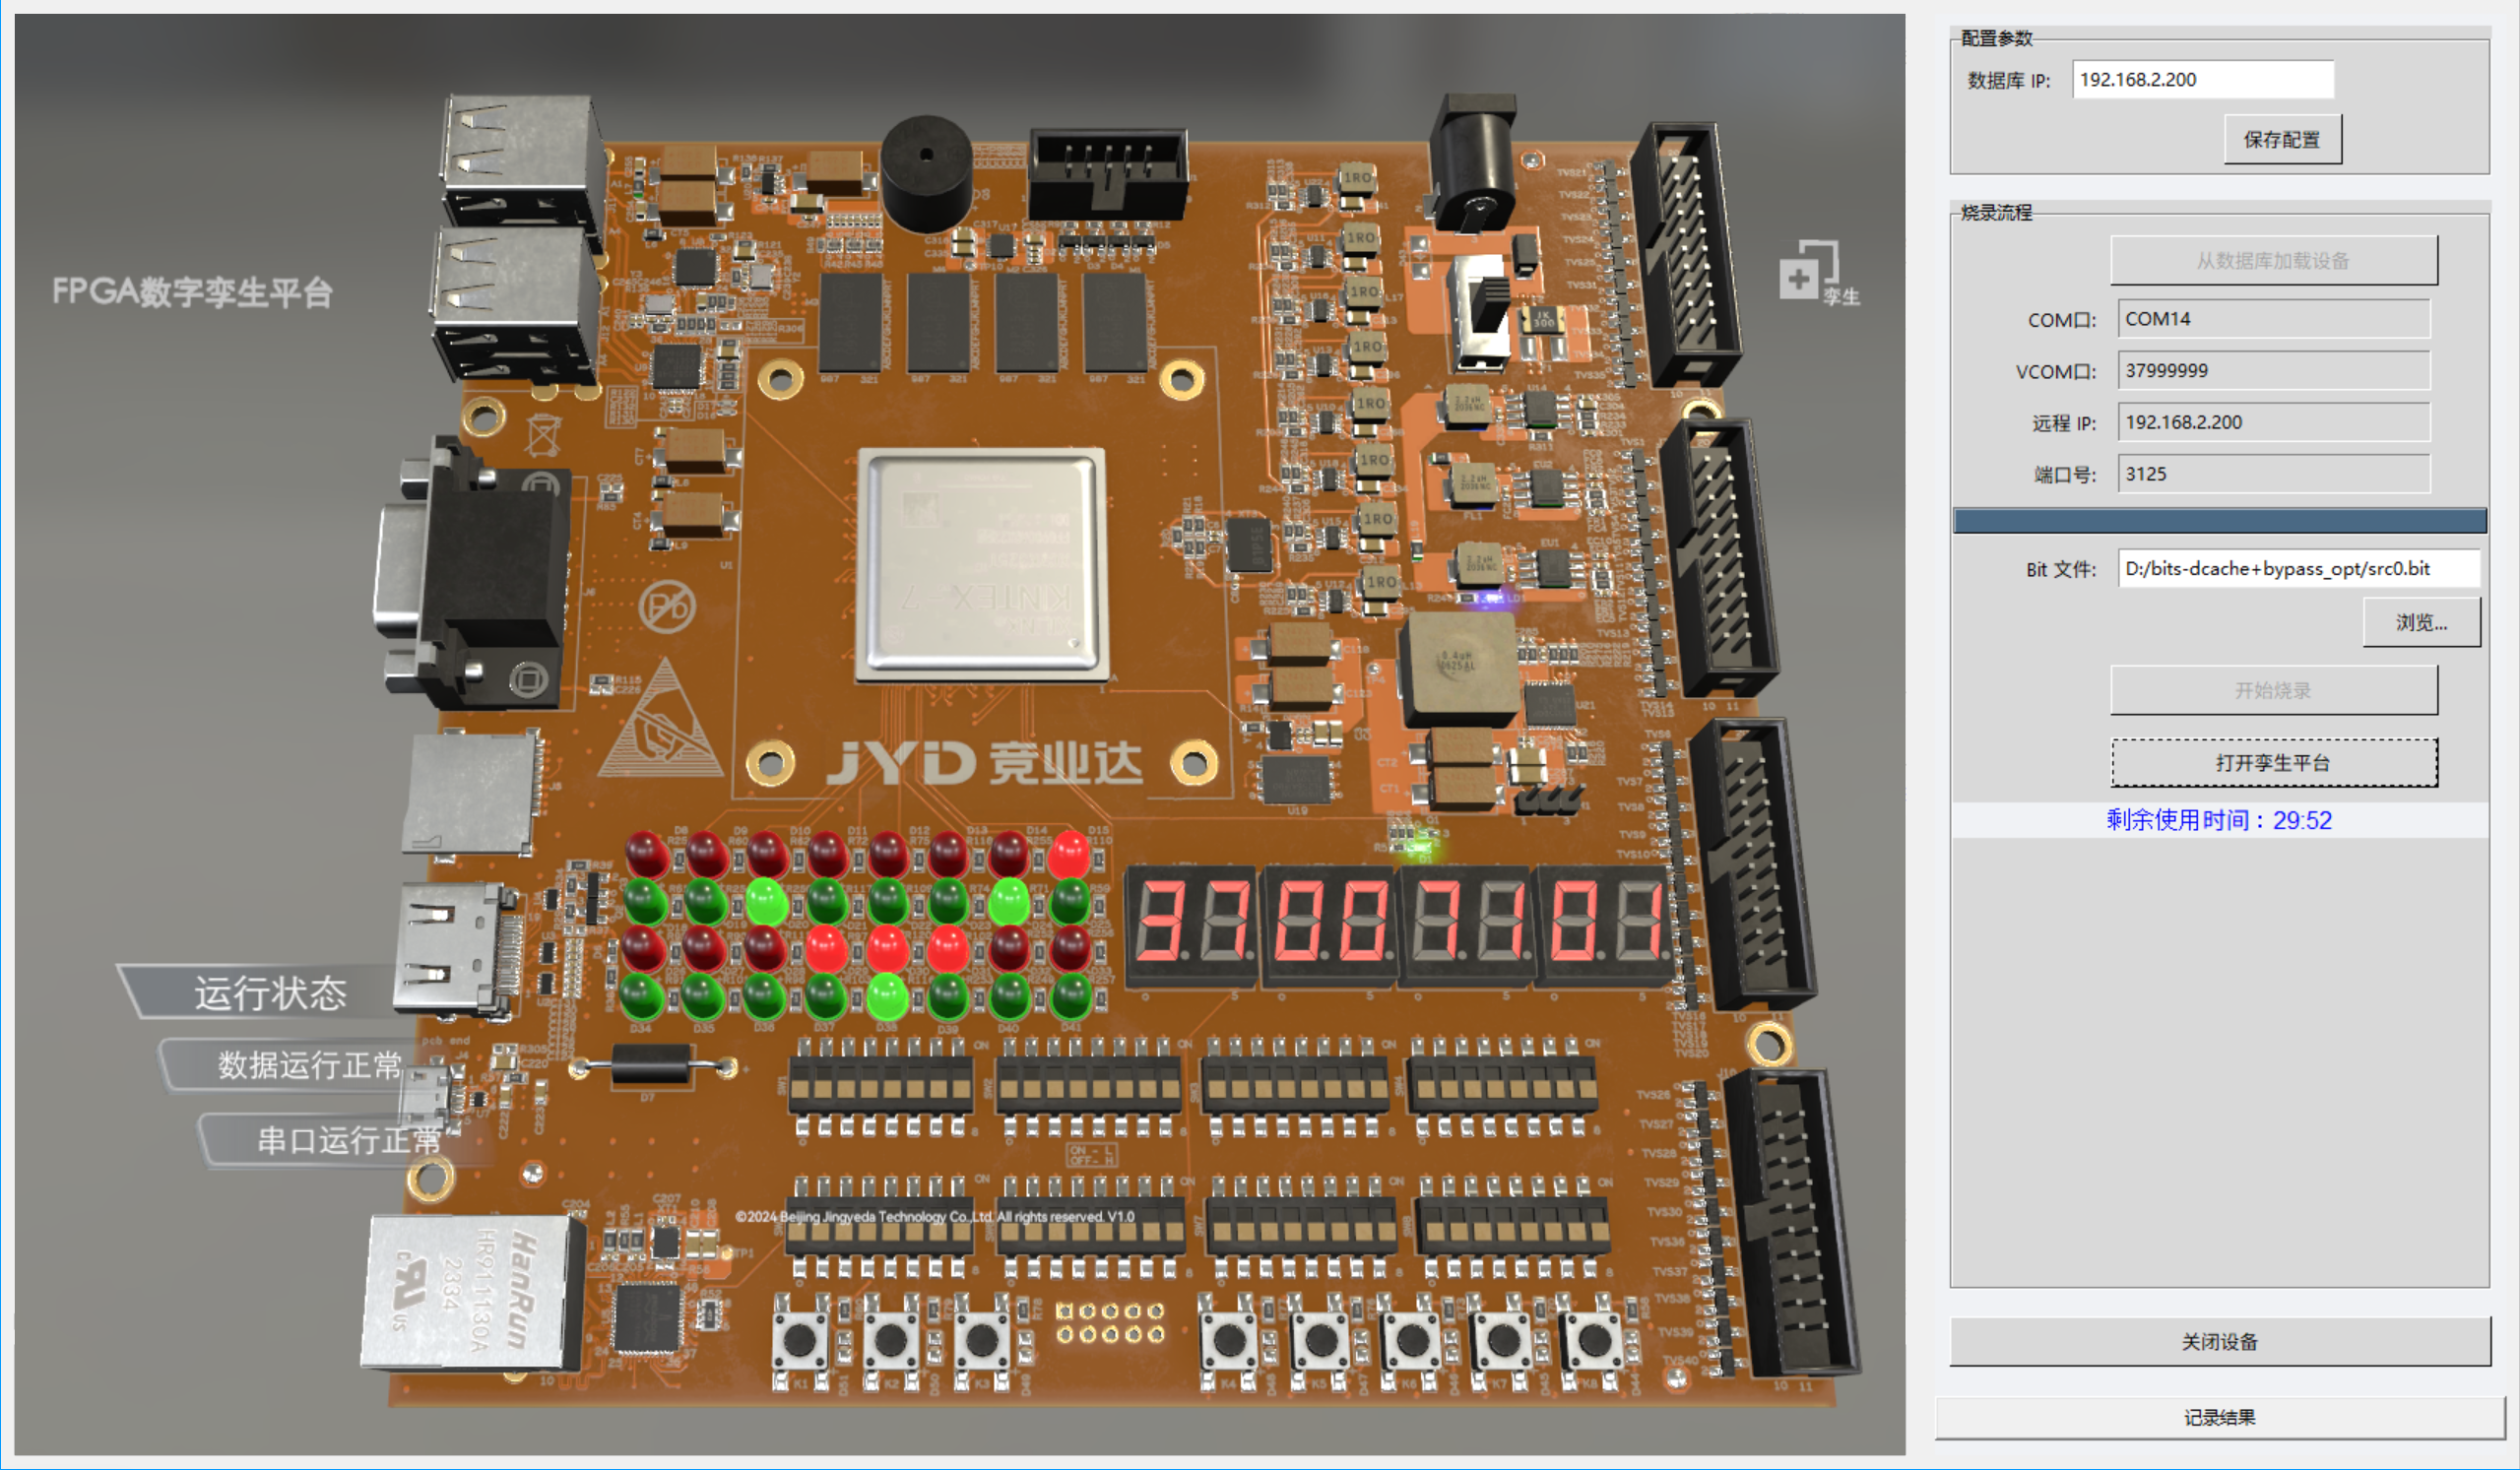
\includegraphics[width=\linewidth]{verify/board/src0.png}
  \caption{src0 上板测试结果（7.101s）}
\end{figure}

\begin{figure}[H]
  \centering
  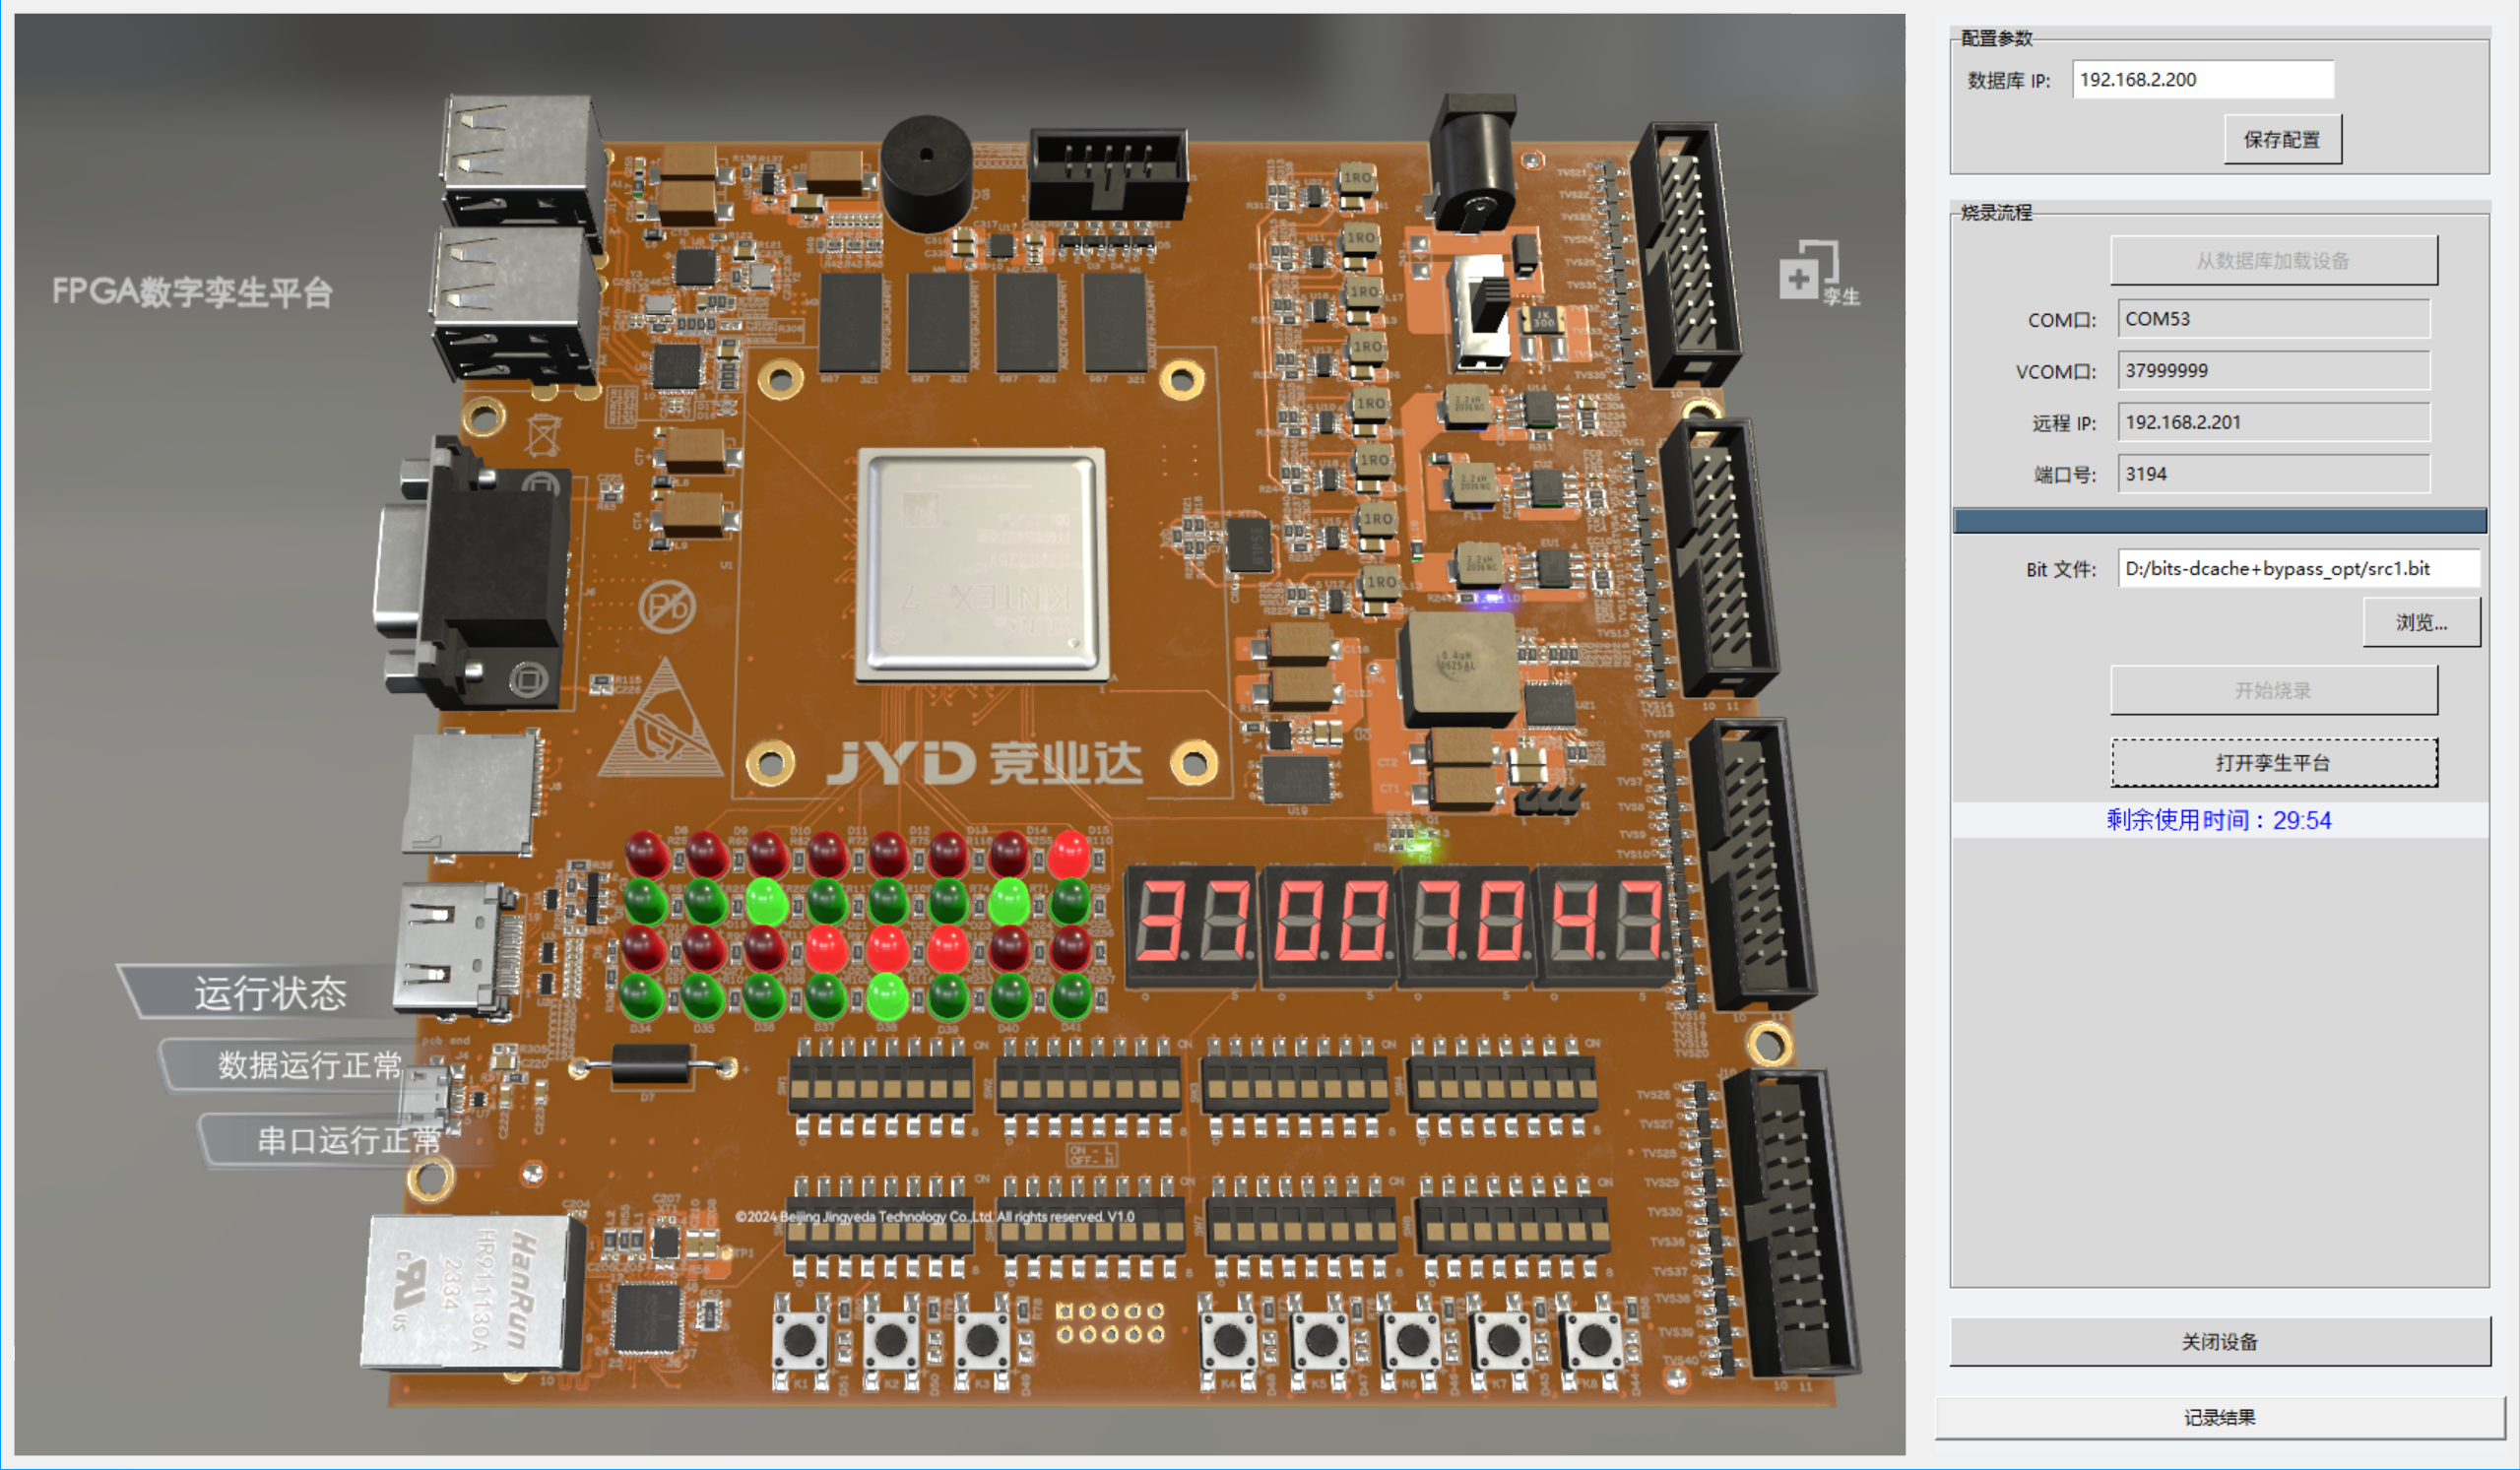
\includegraphics[width=\linewidth]{verify/board/src1.png}
  \caption{src1 上板测试结果（7.047s）}
\end{figure}

\begin{figure}[H]
  \centering
  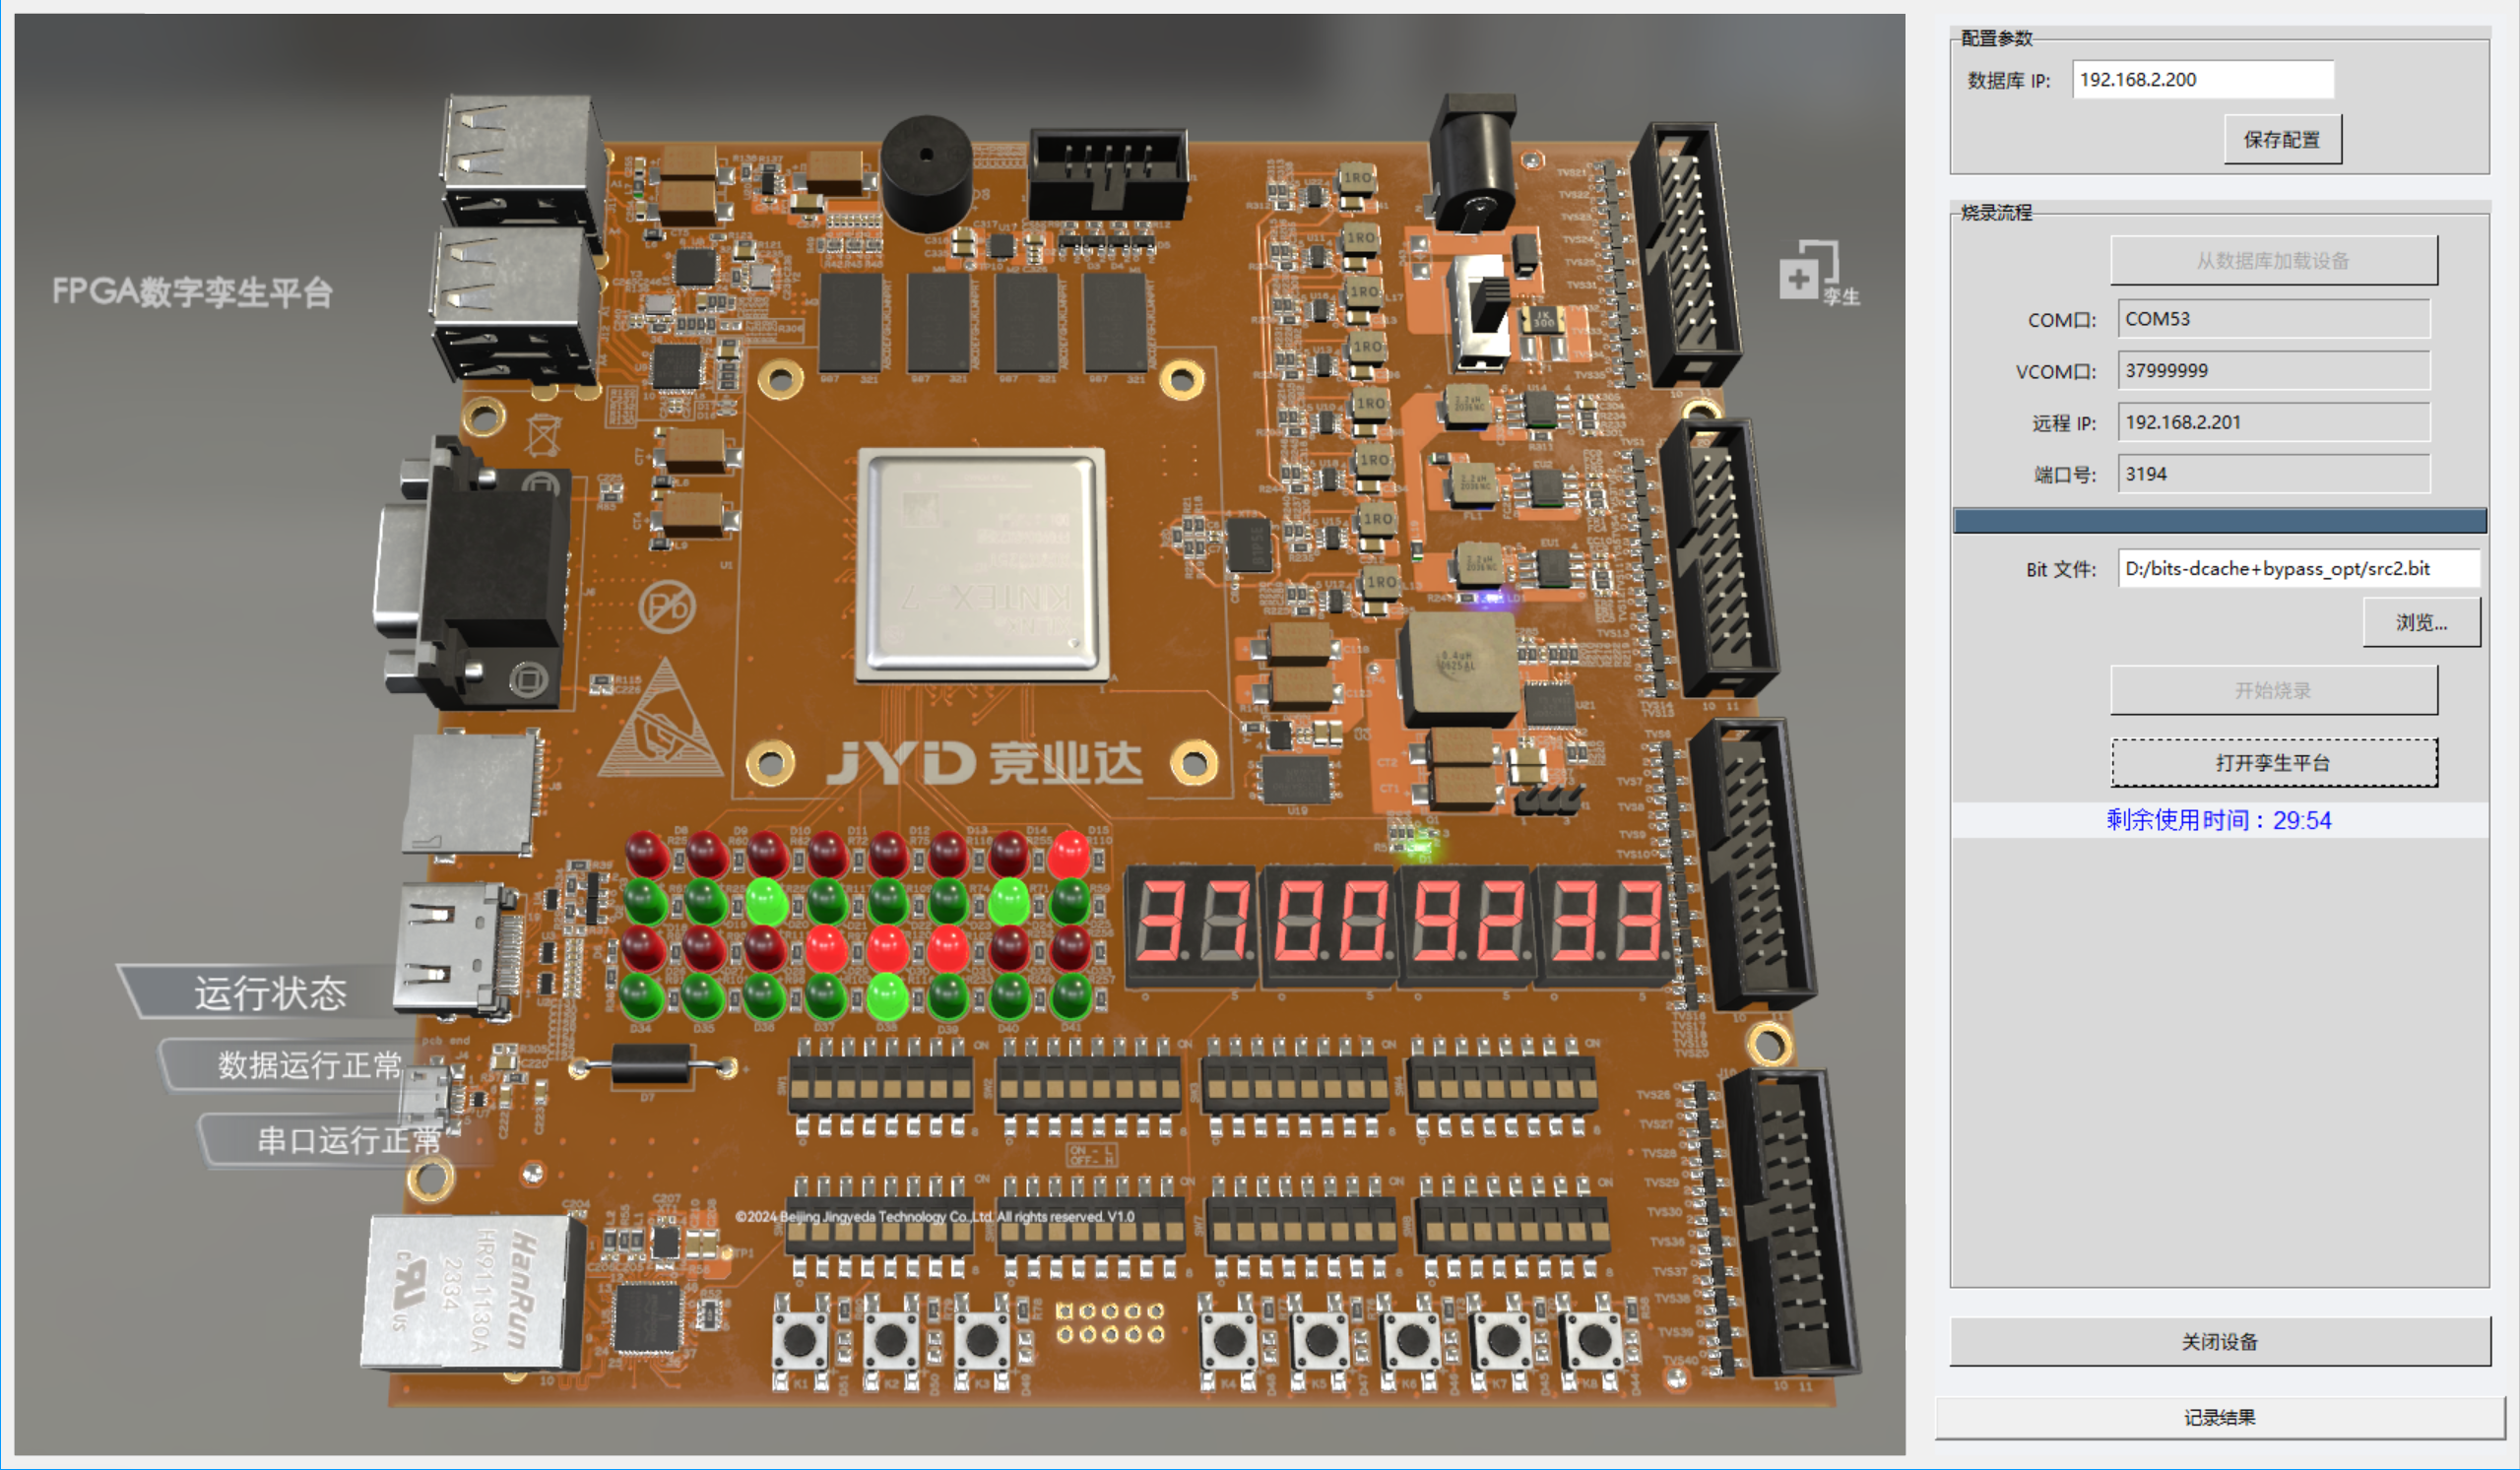
\includegraphics[width=\linewidth]{verify/board/src2.png}
  \caption{src2 上板测试结果（9.233s）}
\end{figure}

\begin{figure}[H]
  \centering
  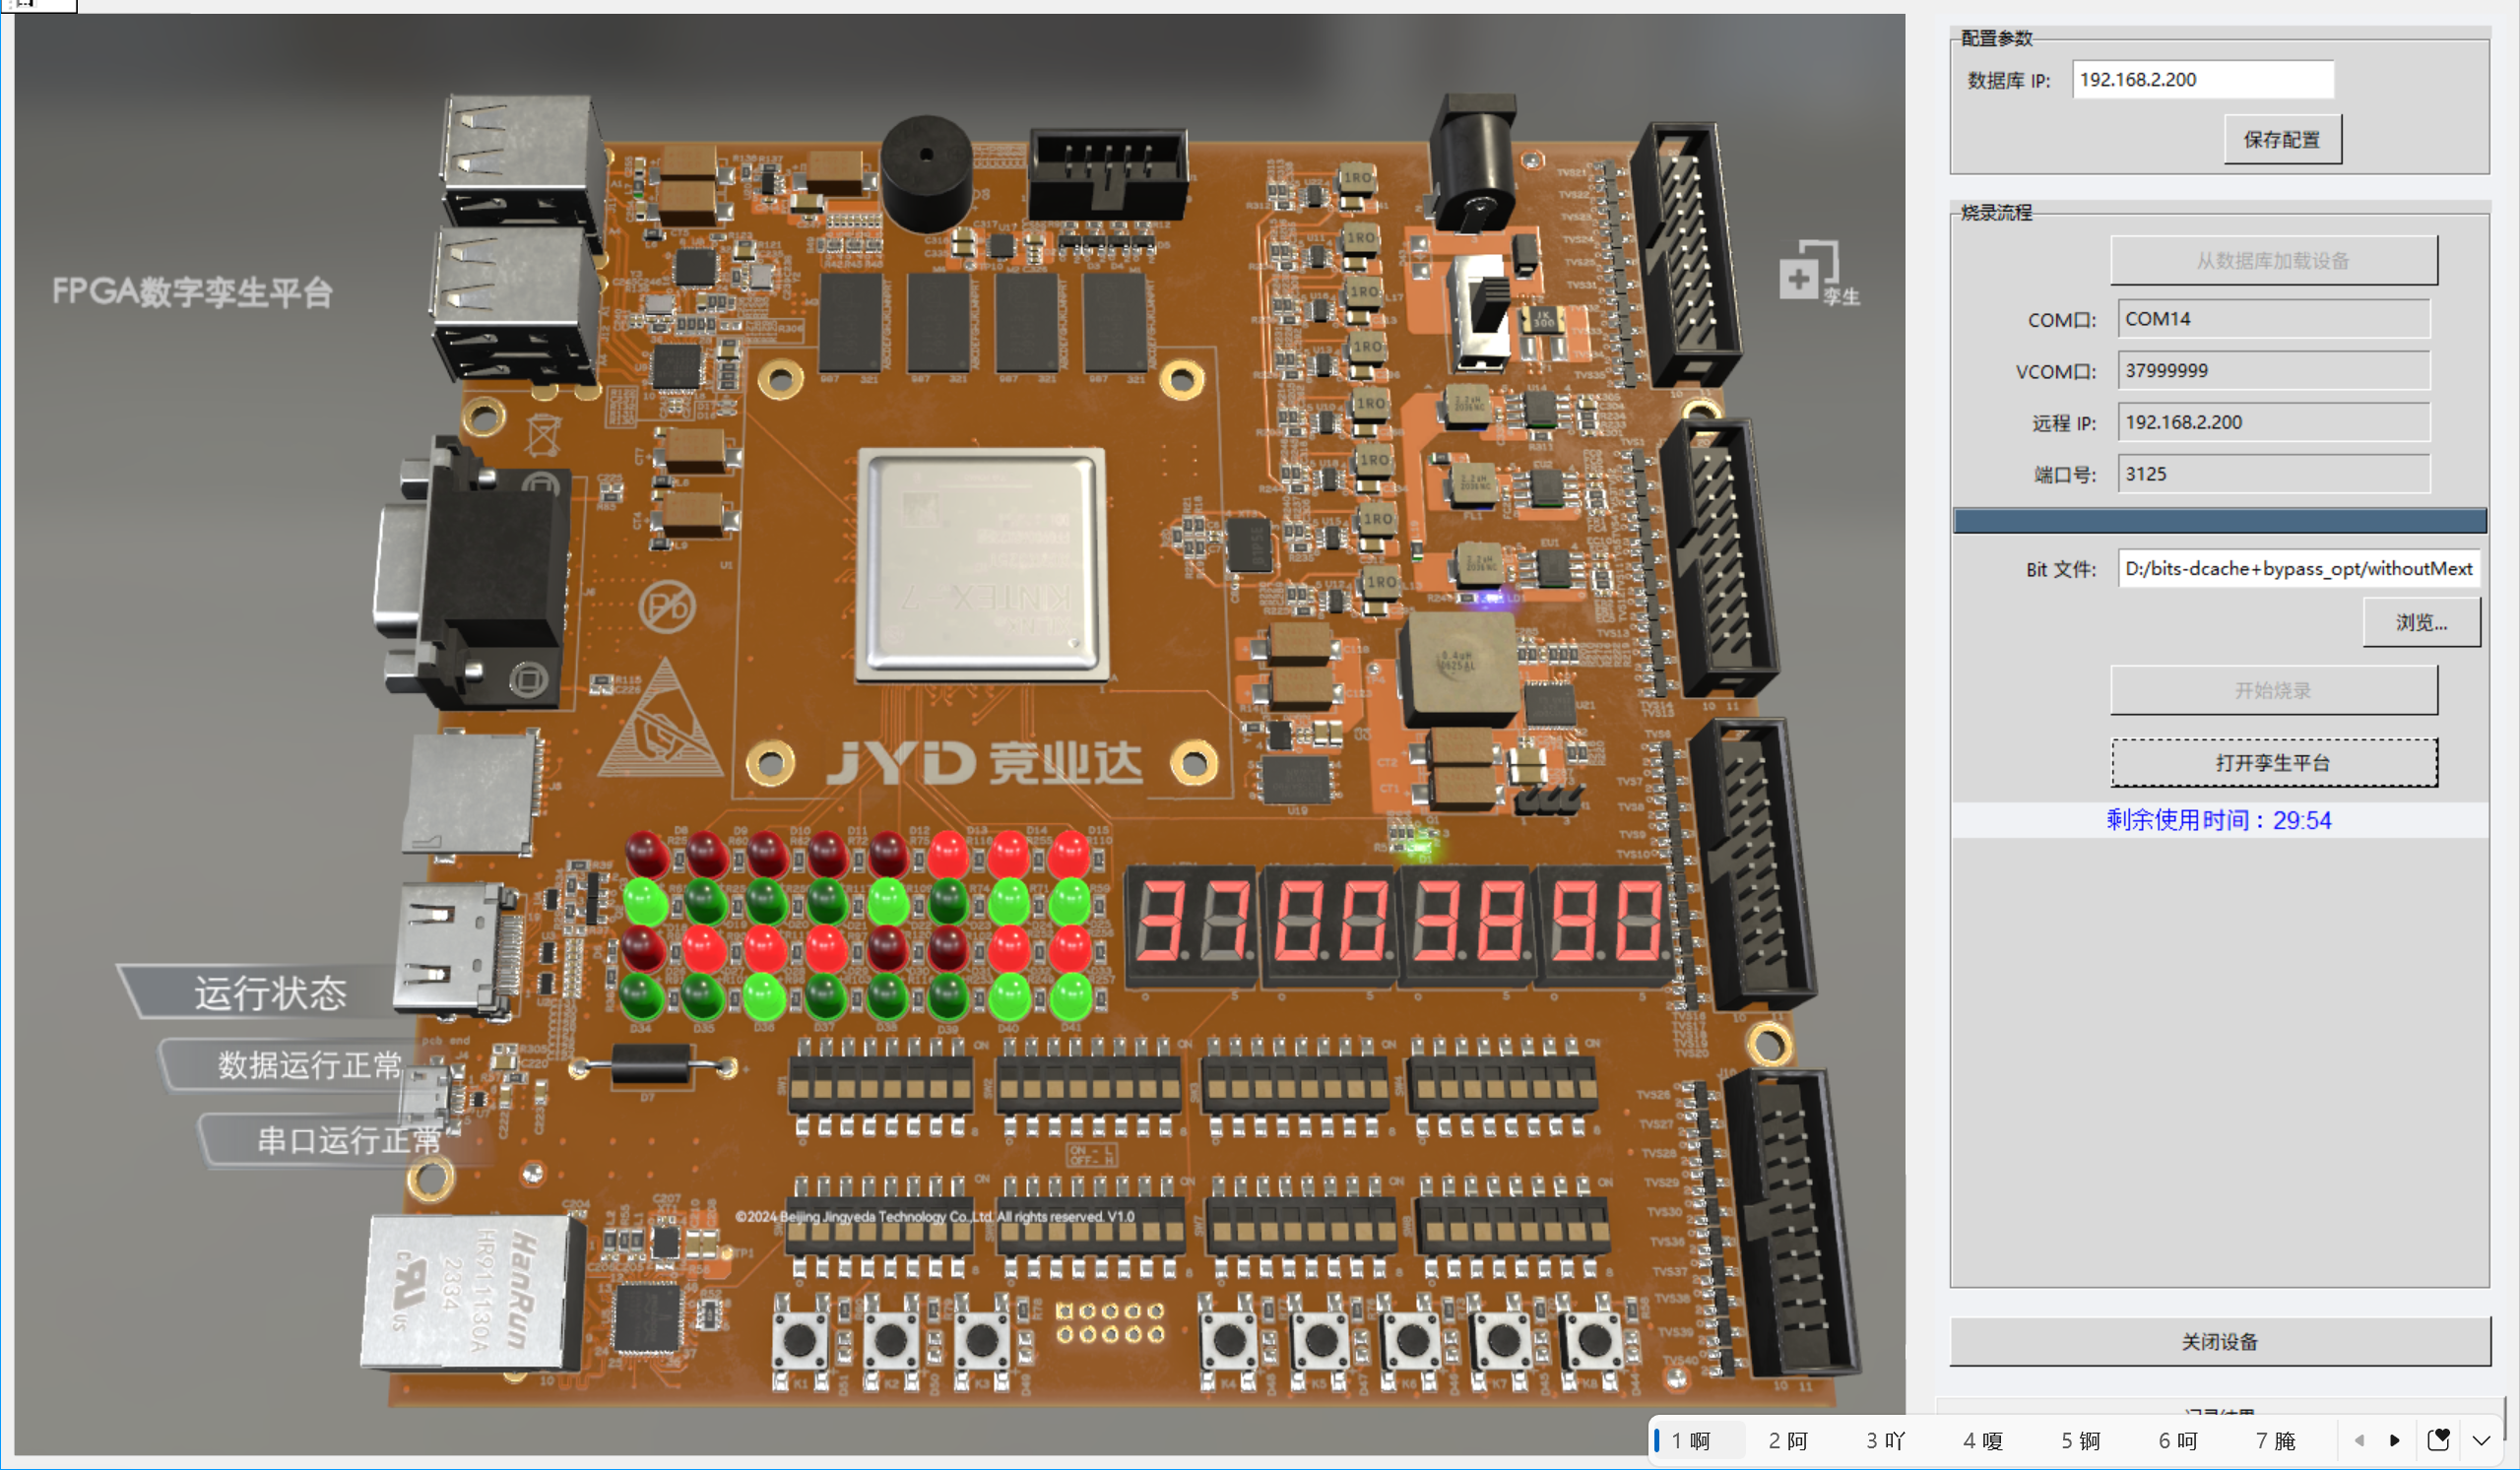
\includegraphics[width=\linewidth]{verify/board/withoutMext.png}
  \caption{withoutMext 上板测试结果（3.890s）}
\end{figure}

\begin{figure}[H]
  \centering
  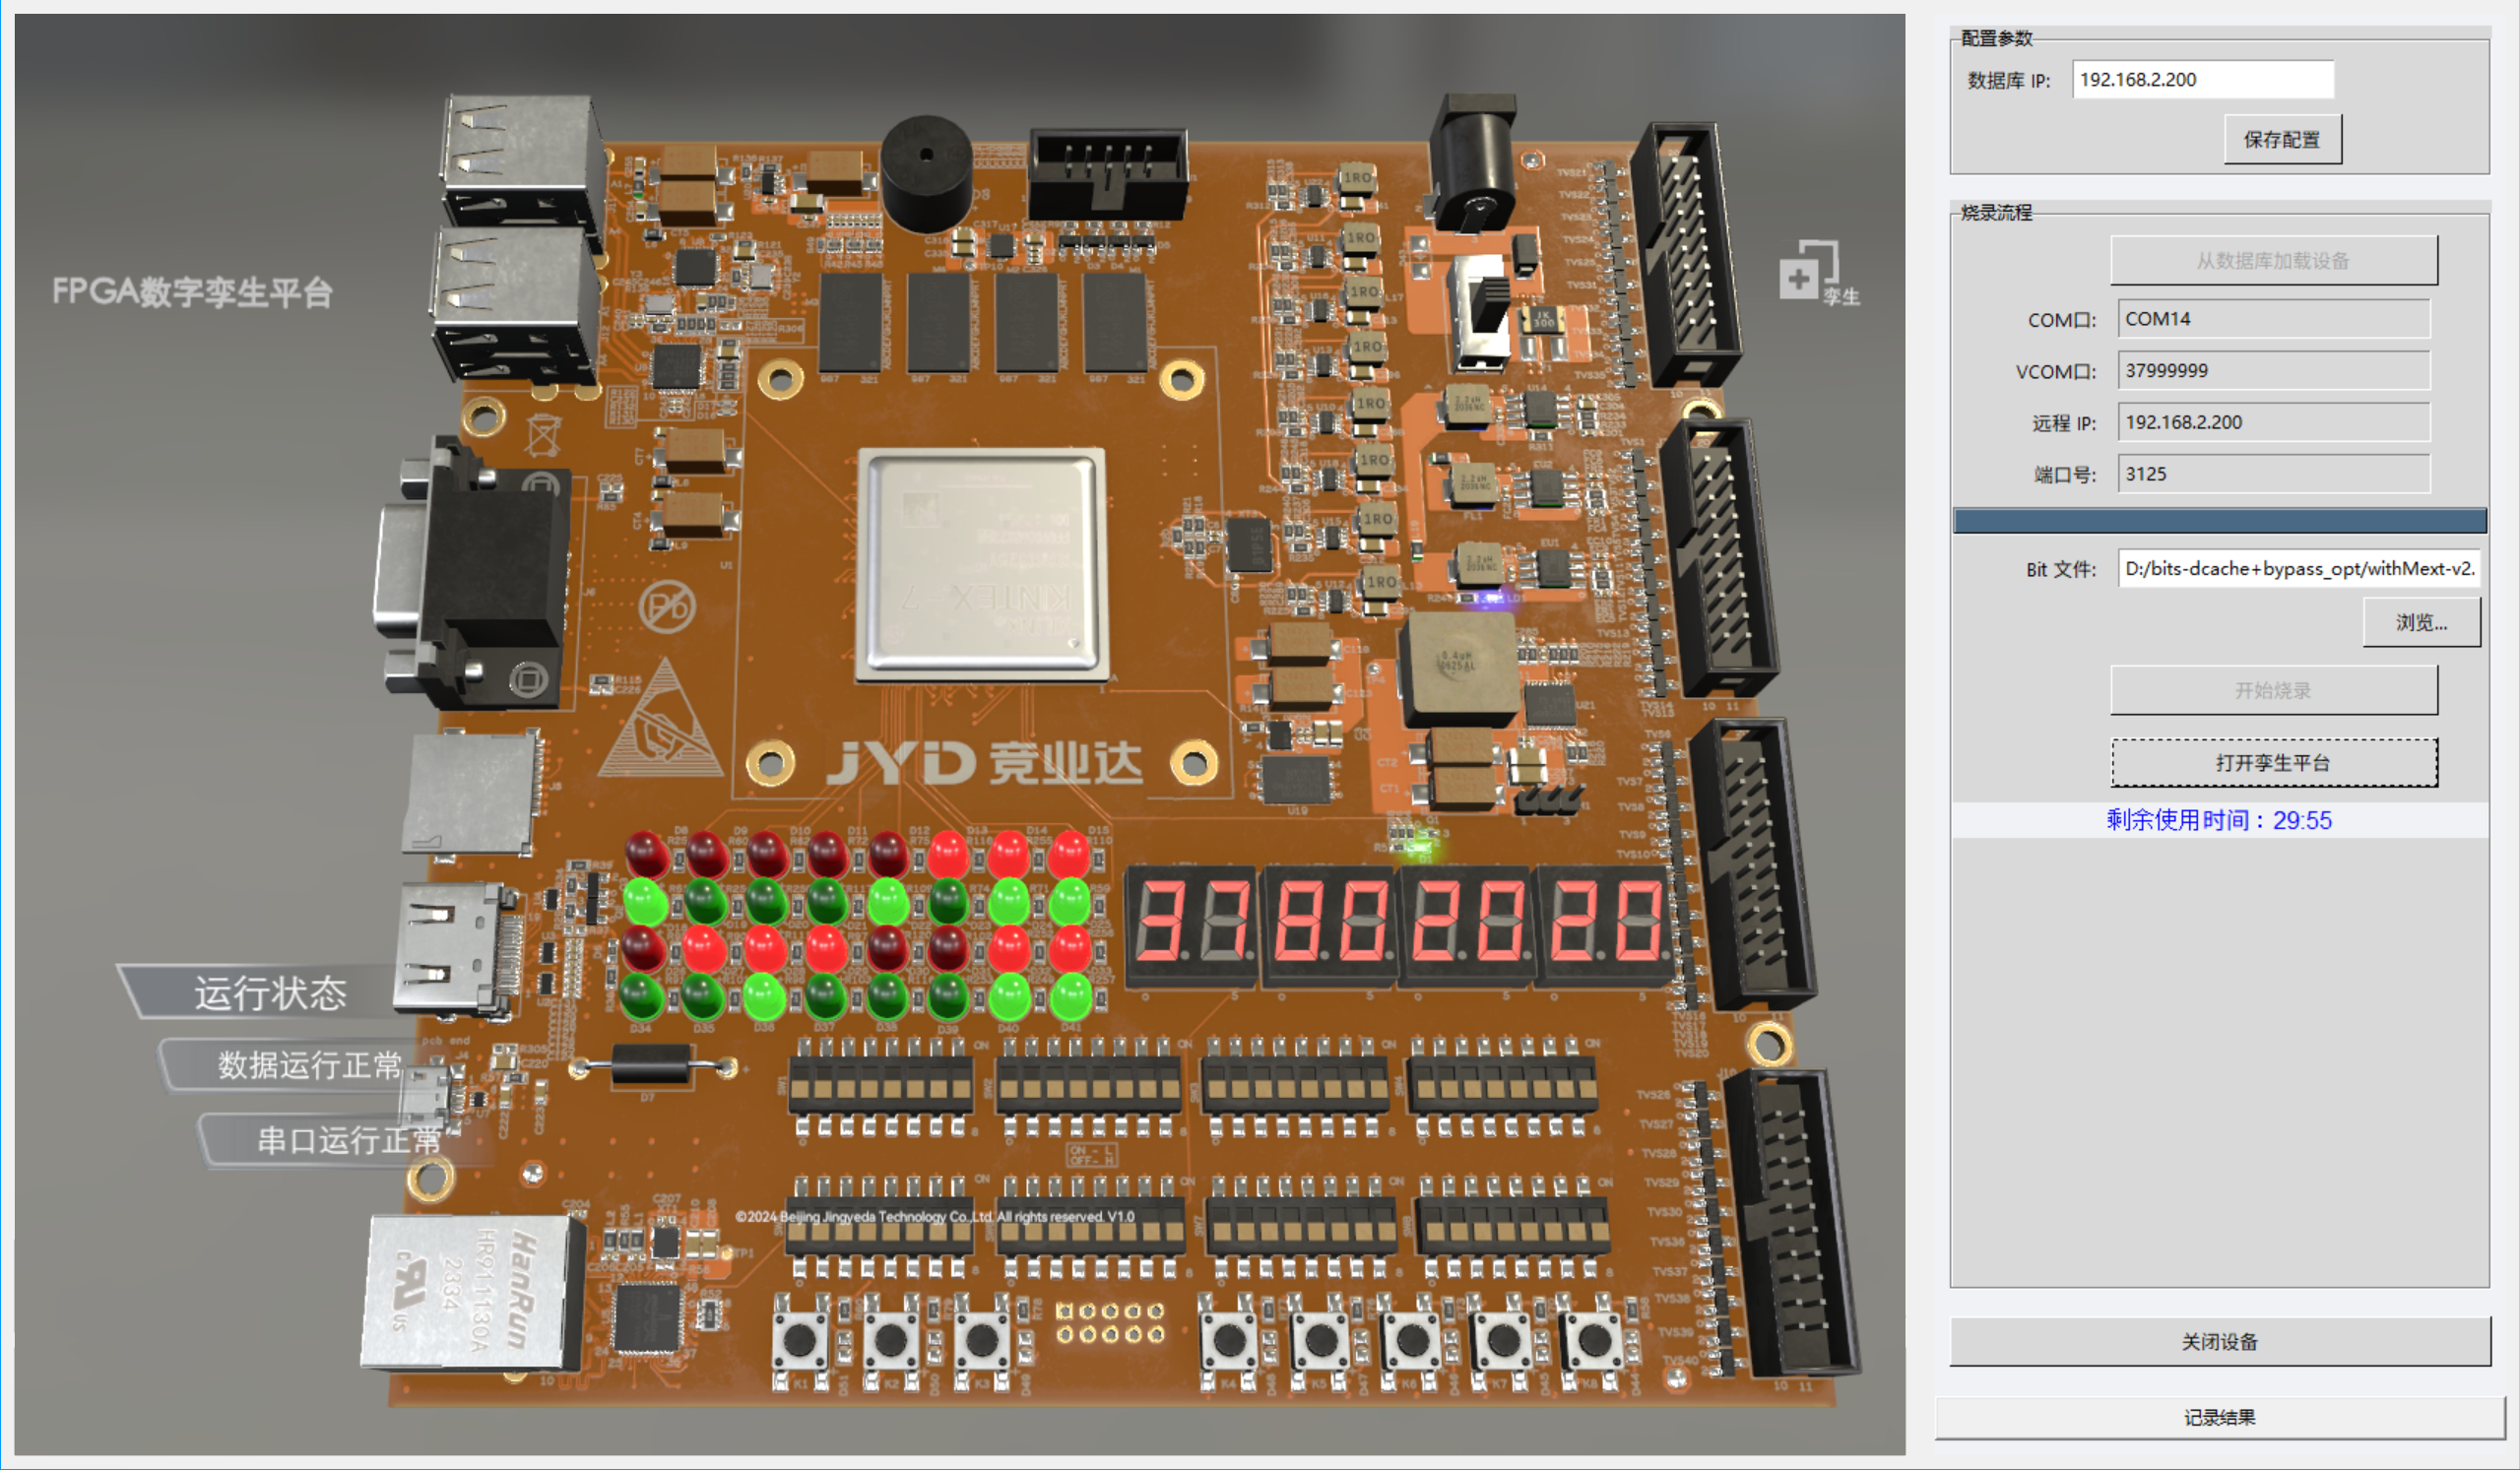
\includegraphics[width=\linewidth]{verify/board/withMext.png}
  \caption{withMext 上板测试结果（2.020s）}
\end{figure}

从上述截图可以看到，平台已经成功加载开发板并打开孪生界面，状态栏显示运行正常；同时 LED 阵列与数码管给出了各自的显示结果，说明对应程序在板端完成执行且运行正确。

\subsection{280 MHz 时序收敛说明}

工程在 Vivado 2024.2 中采用 Performance\_WLBlockPlacement 作为 implementation strategy 进行布局布线优化。

\begin{figure}[H]
  \centering
  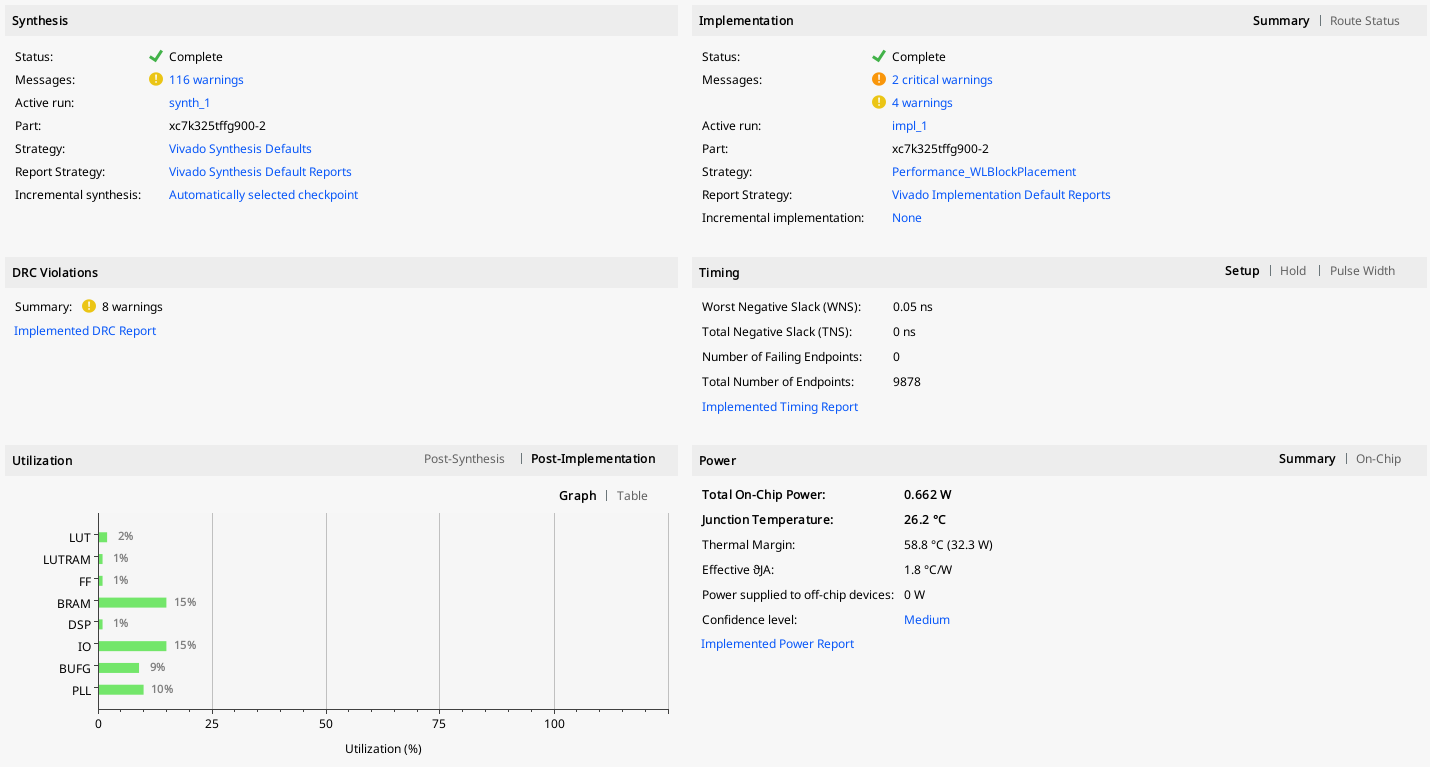
\includegraphics[width=0.96\linewidth]{common/快速预览-1.png}
  \caption{分赛区决赛版本实现与性能快速预览}
\end{figure}

该策略下，工程在 280 MHz 时钟约束下完成综合、实现和 bitstream 生成。布局布线后的最差时序裕量
WNS 为 +0.050 ns，无建立时间违例，说明设计满足 280 MHz 目标频率要求。结合数字孪生平台上五组程序的
实际运行结果，可以说明该版本不仅在工具实现层面通过高频约束，而且在板端运行中保持稳定。

\begin{figure}[H]
  \centering
  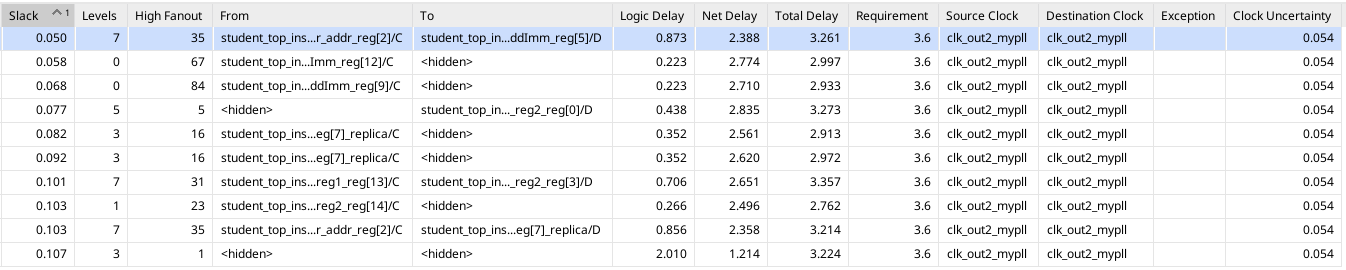
\includegraphics[width=0.96\linewidth]{common/快速预览-slack.png}
  \caption{280 MHz 时钟约束下 WNS 为 +0.050 ns}
\end{figure}

\subsection{RV32I指令支持情况说明}

本项目围绕 RV32I 基本整数指令集进行设计与验证。当前上板用例 src0、src1、src2 在实际运行过程中覆盖了算术逻辑运算、立即数运算、访存访问、条件分支以及 JAL/JALR 等典型执行路径；可以作为本项目支持 RV32I 指令执行能力的佐证。同时，后续的自动化测试流程将通过更全面的测试集验证处理器对 RV32I 的支持。


\newpage

\subsection{验证结果总结说明}

5 份测试用例均在 Vivado 2024.2 下无违例完成实现并成功生成比特流。

\begin{threelongtable}{@{}
  C{0.13\linewidth}
  C{0.29\linewidth}
  C{0.11\linewidth}
  C{0.16\linewidth}
  C{0.13\linewidth}@{}}
\caption{分赛区决赛上板测试结果}\\
\toprule
\textbf{测试用例} & \textbf{数字孪生平台状态} & \textbf{结果} & \textbf{性能测试用时} & \textbf{性能倍率}\footnotemark \\
\midrule
\endfirsthead
\toprule
\textbf{测试用例} & \textbf{数字孪生平台状态} & \textbf{结果} & \textbf{性能测试用时} & \textbf{性能倍率} \\
\midrule
\endhead
\bottomrule
\endlastfoot
src0 & 上板成功，界面运行正常 & 通过 & 7.101s & 4.00 \\
src1 & 上板成功，界面运行正常 & 通过 & 7.047s & 3.70 \\
src2 & 上板成功，界面运行正常 & 通过 & 9.233s & 4.00 \\
withoutMext & 上板成功，界面运行正常 & 通过 & 3.890s & --- \\
withMext & 上板成功，界面运行正常 & 通过 & 2.020s & 1.93\textsuperscript{*} \\
\end{threelongtable}
\footnotetext{src0、src1、src2 相对于赛题给出的 50 MHz 单周期参考设计；带 * 的 1.93 表示
withMext 相对于 withoutMext 的加速比。}

综上，分赛区决赛工程已经完成从设计实现、bitstream 生成到数字孪生上板验证的全流程闭环。
五组程序均在 280 MHz 下观察到正确运行结果，说明 CPU、FPGA 顶层封装、IROM/DRAM 初始化、
MMIO 输出路径及 RV32M 多周期乘除法单元工作正常。

\newpage

\clearpage
\section{总结}

本项目完成了一款面向竞业达 FPGA 平台的五级流水 RISC-V CPU，并在初赛版本基础上扩展了
RV32M、Zicsr 与机器态控制流支持。处理器通过 ready/valid 反压、数据旁路、RAW 相关停顿和统一
重定向机制维持顺序提交；多周期乘除法、BRAM 存储、2 KiB D-cache、分布式 RAM 寄存器堆和
16 项 BTB 等设计共同改善了功能覆盖、物理时序和有效吞吐率。

验证工作覆盖指令级单元测试、小规模程序、官方性能测试、CoreMark、Dhrystone、RT-Thread 基础负载
以及五组数字孪生上板用例。Vivado Simulation 与 Verilator/NEMU 差分验证互为补充，自动化流程能够
持续检查正确性并统计周期数、指令数、IPC、CPI、分支预测准确率和 RAW 阻塞率；仿真计算的官方程序
运行时间与上板显示一致，说明验证结果具有较高可信度。

最终工程在 Vivado 2024.2 下达到 280 MHz，WNS 为 +0.050 ns，五组上板程序均运行正确。
结果表明，本项目已形成从体系结构设计、RTL 实现、仿真回归、性能分析、时序收敛到 FPGA 上板的
完整研发闭环，并为后续完善异常中断体系、操作系统支持和更通用的 AXI4 SoC 集成保留了扩展基础。

\appendix
\section{附录}

\subsection{代码清单}

以下代码清单选取生成后 Verilog 中的核心逻辑，并对无关端口、调试信号和重复连线进行了删节，以便展示关键设计思想。

\begin{lstlisting}[style=svcode,caption={CPUCore.sv / CPUCore：预测错误后的重定向与流水线冲刷}]
wire redirectNow = _exu_io_out_valid & _exu_io_predWrong;
wire redirectPendingFire = _ifu_io_pc_ready & redirectPendingReg;

always @(posedge clock) begin
  if (reset) begin
    redirectPendingReg <= 1'h0;
    pc <= resetPC;
    validReg_3 <= 1'h0;  // IFU -> IDU
    validReg_4 <= 1'h0;  // IDU -> EXU
    validReg_5 <= 1'h0;  // EXU -> LSU
    validReg_6 <= 1'h0;  // LSU -> WBU
  end
  else begin
    redirectPendingReg <= redirectNow
      | (~redirectPendingFire & redirectPendingReg);

    if (_ifu_io_pc_ready)
      pc <= redirectNow ? _exu_io_nxtPC
        : redirectPendingFire | ~redirectPendingReg
            ? nxtPredictedPC
            : redirectTargetReg;

    validReg_3 <= allowIn_3
      ? _ifu_io_out_valid & ~activeRedirectValid
      : ~activeRedirectValid & validReg_3;
    validReg_4 <= allowIn_4
      ? _idu_io_out_valid & ~redirectNow
      : ~redirectNow & validReg_4;
  end

  if (redirectNow)
    redirectTargetReg <= _exu_io_nxtPC;
end
\end{lstlisting}

\begin{lstlisting}[style=svcode,caption={IDU.sv / IDU：CSR 读取与静态跳转目标预选}]
assign io_csrRead_en = io_in_valid;
assign io_csrRead_addr = io_in_bits_code[31:20];

assign io_out_bits_info_csrReadData = io_csrRead_data;
assign io_out_bits_info_staticNextPCOrCSRTarget =
  io_out_bits_info_isECall_0
    ? io_csrJmpTarget_mtvec
    : io_out_bits_info_isMRet_0
        ? io_csrJmpTarget_mepc
        : io_in_bits_pc + 32'h4;

assign io_out_bits_info_pcAddImm = io_in_bits_pc
  + io_out_bits_info_imm_0;
assign io_out_bits_info_reg1AddImm = _bypassMux_io_outData1
  + {{21{io_in_bits_code[31]}}, io_in_bits_code[30:20]};
\end{lstlisting}

\begin{lstlisting}[style=svcode,caption={EXU.sv / EXU：跳转判定、预测错误与 CSR 写回}]
wire isCSRRW = io_in_bits_code[14:12] == 3'h1
  & io_in_bits_info_typ[8];
wire dbgIsCSRJmp = io_in_bits_info_isECall
  | io_in_bits_info_isMRet;

assign io_jmpHappen =
  (dbgIsBranch & takeBranch) | dbgIsJALR | dbgIsJAL | dbgIsCSRJmp;
assign io_predWrong =
  dbgIsJALR | dbgIsCSRJmp
  | (isBranch & (takeBranch ^ io_in_bits_pred_take))
  | (dbgIsJAL & ~io_in_bits_pred_hit);

assign io_nxtPC =
  dbgIsJALR ? {io_in_bits_info_reg1AddImm[31:1], 1'h0}
  : (dbgIsJAL | isTakenBranch) ? io_in_bits_info_pcAddImm
  : io_in_bits_info_staticNextPCOrCSRTarget;

assign io_out_bits_exuWriteBack_csr_en =
  isCSRRW | (isCSRRS & (|io_in_bits_info_reg1));
assign io_out_bits_exuWriteBack_csr_addr =
  io_in_bits_info_isECall ? 12'h341 : io_in_bits_code[31:20];
assign io_out_bits_exuWriteBack_csr_data =
  io_in_bits_info_isECall ? io_in_bits_pc
  : isCSRRW ? io_in_bits_info_reg1
  : io_in_bits_info_csrReadData | io_in_bits_info_reg1;
\end{lstlisting}

\begin{lstlisting}[style=svcode,caption={DualSimpleBusToAXI4.sv / DualSimpleBusToAXI4：双 SimpleBus 到 AXI4 的桥接}]
reg [2:0] state;
reg       selLSU;
reg [31:0] reqAddr, reqWData;
reg [2:0]  reqSize;
reg [3:0]  reqWMask;
reg        awSent, wSent;

wire hasReq = io_lsu_req_valid | io_ifu_req_valid;
wire takeLSU = io_lsu_req_valid;

assign io_lsu_req_ready = state == 3'h0;
assign io_ifu_req_ready = (state == 3'h0) & ~takeLSU;

always @(posedge clock) begin
  if (reset)
    state <= 3'h0;
  else begin
    casez (state)
      3'h0: state <= hasReq ? (takeLSU && io_lsu_wen ? 3'h3 : 3'h1) : 3'h0;
      3'h1: state <= io_out_arready ? 3'h2 : 3'h1;
      3'h2: state <= io_out_rvalid  ? 3'h0 : 3'h2;
      3'h3: state <= (awSent | io_out_awready) & (wSent | io_out_wready)
                      ? 3'h4 : 3'h3;
      3'h4: state <= io_out_bvalid  ? 3'h0 : 3'h4;
    endcase
  end
end

assign io_out_arvalid = state == 3'h1;
assign io_out_rready  = state == 3'h2;
assign io_out_awvalid = (state == 3'h3) & ~awSent;
assign io_out_wvalid  = (state == 3'h3) & ~wSent;
assign io_out_bready  = state == 3'h4;
\end{lstlisting}

\begin{lstlisting}[style=svcode,caption={CPUTop.sv / CPUTop：CPUCore 接入 AXI4 桥接模块}]
CPUCore core (
  .io_irom_req_ready  (_memBridge_io_ifu_req_ready),
  .io_irom_req_valid  (_core_io_irom_req_valid),
  .io_irom_addr       (_core_io_irom_addr),
  .io_irom_resp_valid (_memBridge_io_ifu_resp_valid),
  .io_irom_rdata      (_memBridge_io_ifu_rdata),
  .io_dram_req_ready  (_memBridge_io_lsu_req_ready),
  .io_dram_req_valid  (_core_io_dram_req_valid),
  .io_dram_addr       (_core_io_dram_addr),
  .io_dram_wdata      (_core_io_dram_wdata),
  .io_dram_wmask      (_core_io_dram_wmask),
  .io_dram_wen        (_core_io_dram_wen)
);

DualSimpleBusToAXI4 memBridge (
  .io_ifu_req_valid (_core_io_irom_req_valid),
  .io_ifu_addr      (_core_io_irom_addr),
  .io_lsu_req_valid (_core_io_dram_req_valid),
  .io_lsu_addr      (_core_io_dram_addr),
  .io_lsu_wdata     (_core_io_dram_wdata),
  .io_lsu_wmask     (_core_io_dram_wmask),
  .io_lsu_wen       (_core_io_dram_wen),
  .io_out_awvalid   (io_master_awvalid),
  .io_out_awaddr    (io_master_awaddr),
  .io_out_wvalid    (io_master_wvalid),
  .io_out_wdata     (io_master_wdata),
  .io_out_arvalid   (io_master_arvalid),
  .io_out_araddr    (io_master_araddr),
  .io_out_rready    (io_master_rready)
);
\end{lstlisting}

\subsection{工程目录结构}

\makeatletter
\newcommand{\mydotfill}{%
  \leavevmode
  \leaders\hbox to 1em{%
    \hss
    \raisebox{0.3ex}{\textcolor{gray}{.}}%
    \hss
  }\hfill\kern0pt
}
\makeatother

\begin{minipage}{0.9\textwidth}
\centering
\dirtree{%
.1 jyd/ \mydotfill 工程根目录.
.2 npc/ \mydotfill CPU 设计、SoC 封装与仿真工程.
.3 design/src/ \mydotfill Chisel 源码：流水线、总线、外设桥.
.3 build/gened/verilog/ \mydotfill 生成后的 Verilog/SystemVerilog.
.3 sim/ \mydotfill Verilator 仿真与性能统计.
.3 scripts/ \mydotfill 辅助脚本.
.2 jyd-tests/ \mydotfill 竞业达样例程序与 COE 处理脚本.
.2 abstract-machine/ \mydotfill bare-metal 运行环境与平台抽象.
.2 nemu/ \mydotfill RISC-V 参考执行环境.
.2 .github/workflows/ \mydotfill 自动化回归流程.
}
\end{minipage}

\newpage

\subsection{参考资料}

\begin{enumerate}[label={[\arabic*]},leftmargin=3em]
\item 全国大学生集成电路创新创业大赛组委会. 第十届集创赛初赛作品提交要求.
\item 竞业达企业命题组. ``竞业达''企业命题作品材料参考模板.
\item 竞业达企业命题组. FPGA 开发板远程连接操作手册, 2026.
\item 竞业达企业命题组. 上板实验说明与赛题测试程序资料.
\item RISC-V International. The RISC-V Instruction Set Manual, Volume I: Unprivileged ISA.
\item RISC-V International. The RISC-V Instruction Set Manual, Volume II: Privileged Architecture.
\end{enumerate}

\subsection{AI工具使用声明}

工具名称：ChatGPT 5.3/5.4/5.5/5.6。

使用场景与用途如下：

\begin{itemize}
\item 工具脚本编写：自动插入注释、自动修改宏名、将 coe 文件转 bin 并反编译成汇编、自动打包代码、自动移除 dpi 调用、自动替换 Vivado 工程文件为新 Verilog 代码。
\item 部分功能的实现或重构：根据团队的优化思路快速形成初版改动。
\item 仿真代码的部分重构：使用 AI 重构流水线日志的生成方式。
\item 分析时序报告：辅助解读 Vivado 的时序报告。
\item 辅助撰写技术文档：润色文字表达，辅助图表绘制。
\end{itemize}

AI 生成内容占比估计（文字/代码/设计）：

\begin{itemize}
\item 文字：15\%
\item 代码：10\%
\item 设计：5\%
\end{itemize}

\end{document}
